\chapter{Learned Probabilistic Sun Sensor}
\epigraph{He stepped down, avoiding any long look at her as one avoids long looks at the sun, but seeing her as one sees the sun, without looking.}{Leo Tolstoy, \textit{Anna Karenina}}
\label{ch:sun-bcnn}

\section{Introduction}

Given that we can infer useful uncertainty information from images, is it possible to infer both uncertainty and some other geometric quantity that can aid in egomotion estimation? In this chapter, we present a pseudo-sensor that addresses that question. Namely, we train a deep parametric model (a Bayesian Convolutional Neural Network, or BCNN) to act as a \textit{virtual sun sensor} that aims to reproduce the output of a dedicated sun sensor from a single RGB image. 


\begin{figure*}[h!]
\centering
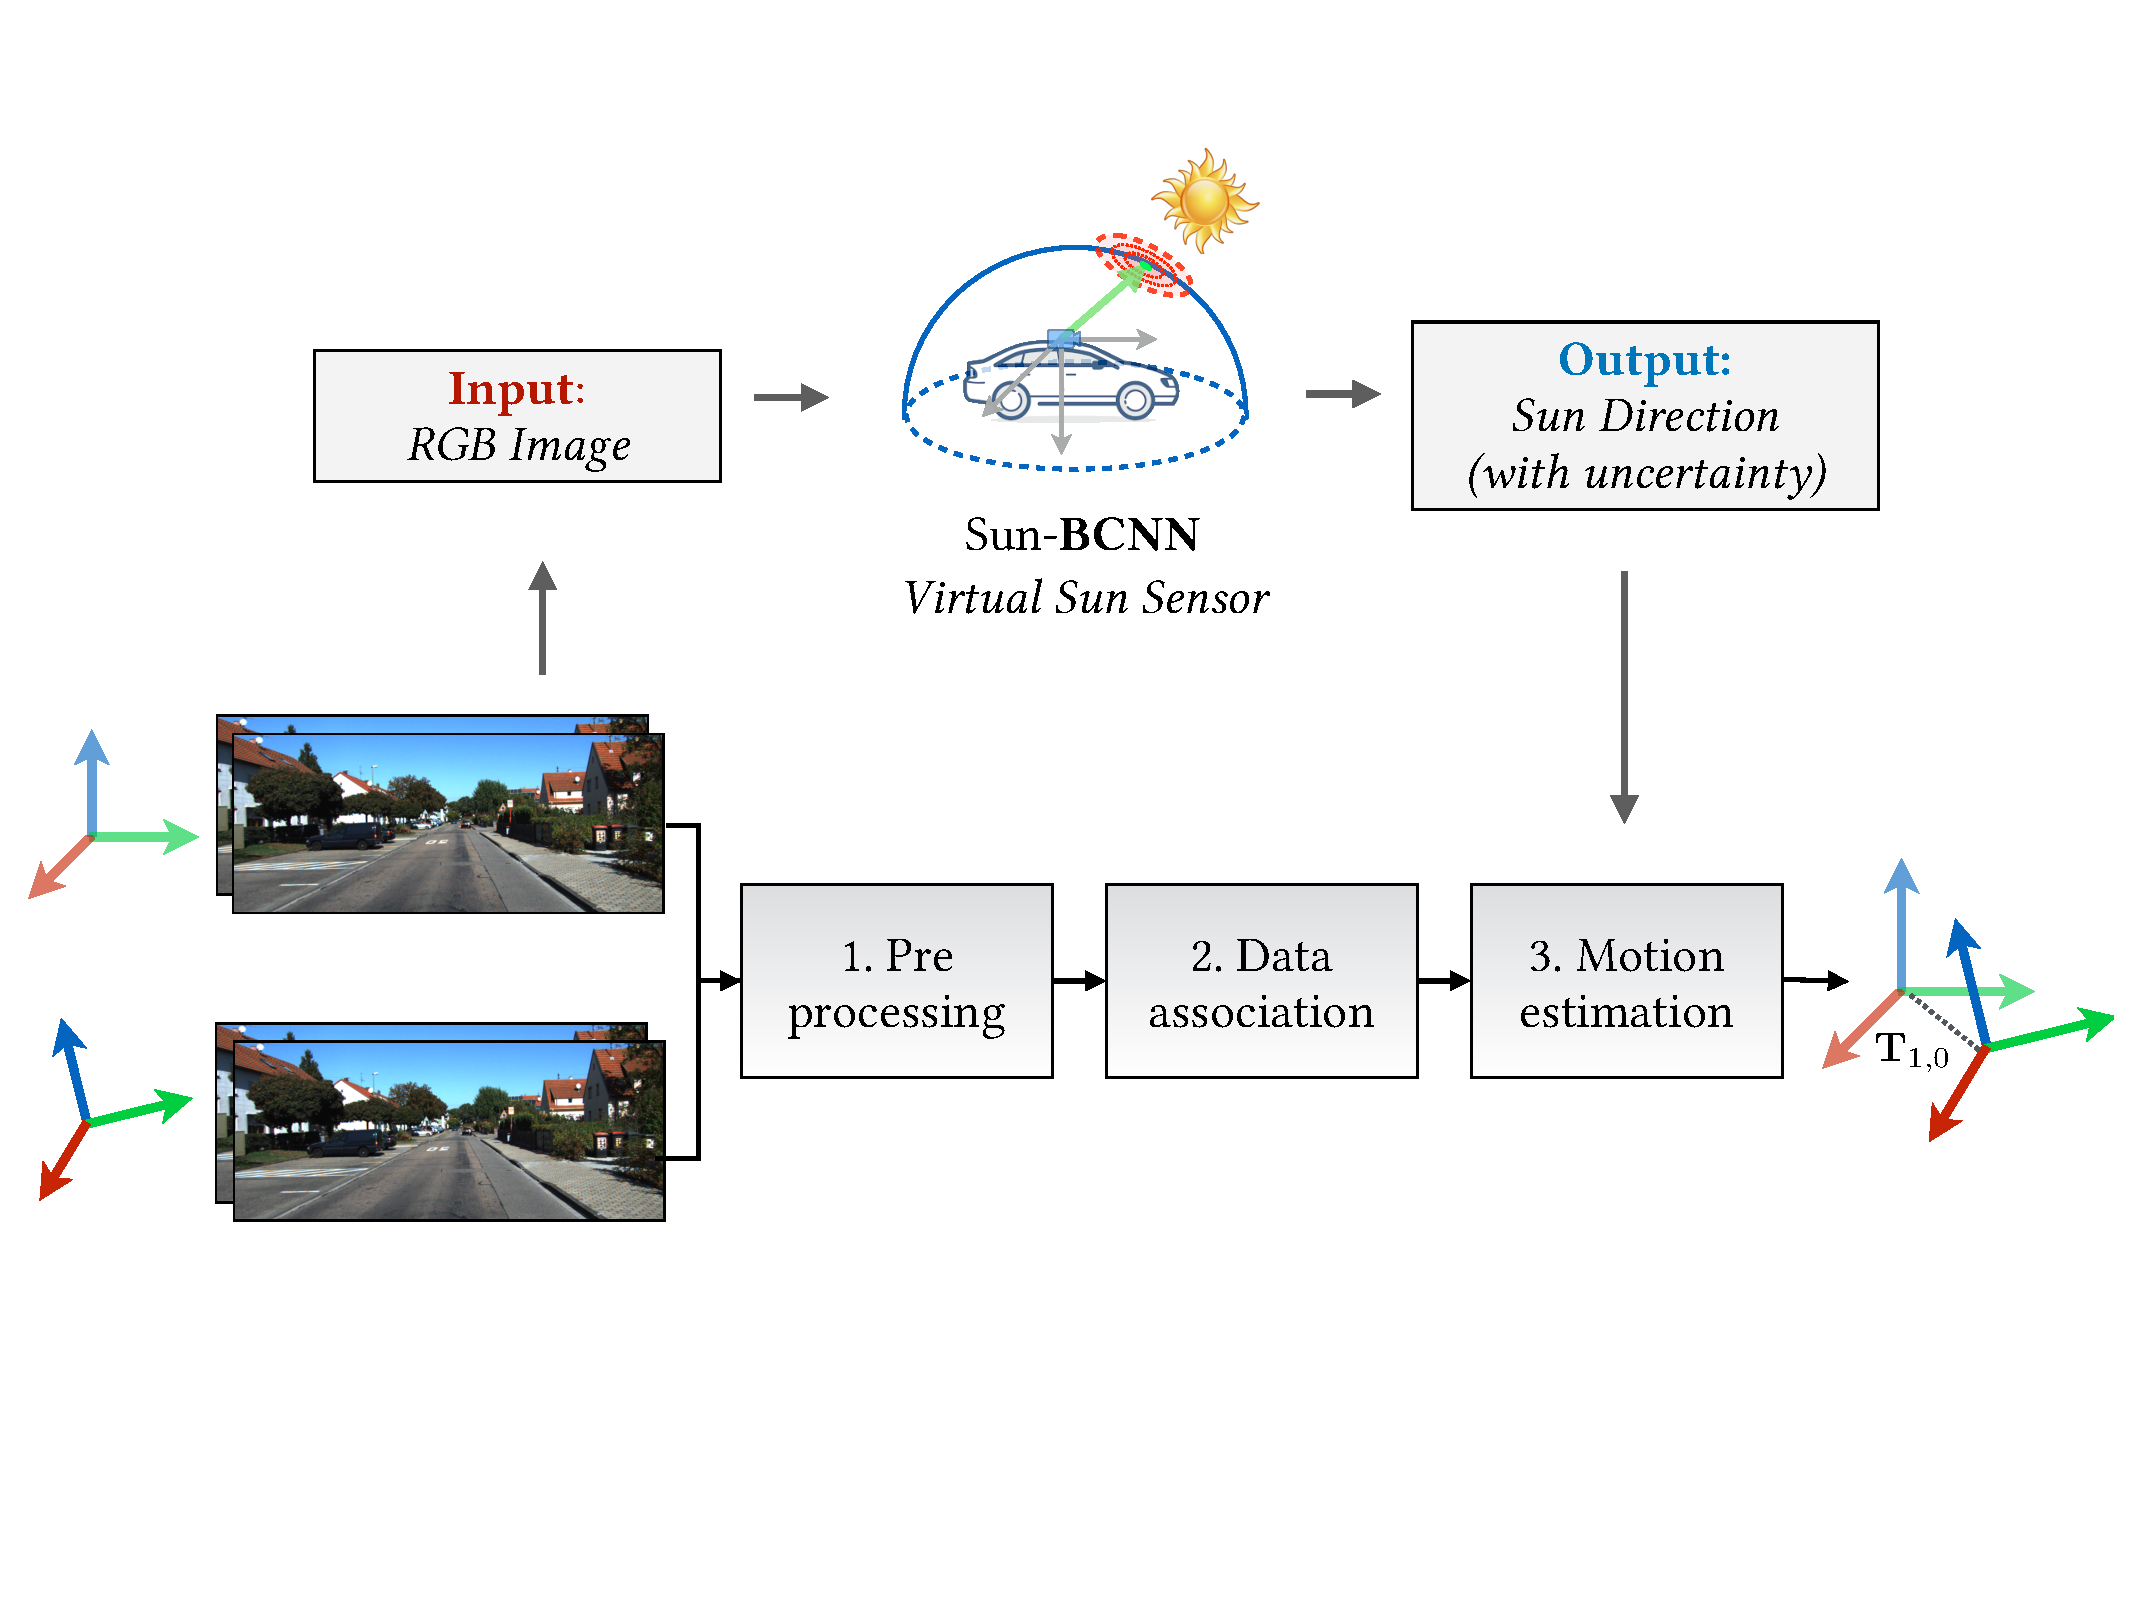
\includegraphics[width=0.8\textwidth]{sun-bcnn.pdf}
 \caption{Sun-BCNN is a learned virtual sun sensor that outputs sun direction with an associated uncertainty based on a single RGB image. We use this as a source of orientation information within a privileged reference frame.}
 \label{fig:sun-bcnn_intro_fig}
\end{figure*}

\begin{remark}{Associated Publications}
This project was a collaboration with Lee Clement. Broadly, Lee lead the integration of sun information into a visual odometry pipeline, while I lead the design and implementation of the BCNN. It is associated with three publications. The first publication was exploratory work on (non-probabilistic) virtual sun sensors lead by Lee,
\begin{enumerate}
\item \bibentry{2017_Clement_Improving},
\end{enumerate}
while the latter two publications were a joint collaboration where I developed and investigated the BCNN formulation and while we collaborated on the experimental validation,
\begin{enumerate}[resume]
\item \bibentry{2017_Peretroukhin_Reducing},
\item \bibentry{2018_Peretroukhin_Inferring}.
\end{enumerate}
This chapter is largely a reproduction of the latter journal publication which summarizes the approach.
\end{remark} 

\section{Motivation}
A crucial competency of any autonomous mobile robot is the ability to estimate its own motion through an operating environment.
While there exists a rich body of literature on the topic of motion estimation using a variety of techniques such as lidar-based point cloud matching \citep{Zhang2015} and visual-inertial odometry \citep{Leutenegger2015-fk}, egomotion estimation is fundamentally a process of dead-reckoning and will accumulate unbounded error over time.

%\begin{wrapfigure}{r}{0.5\textwidth}
%    \centering
%      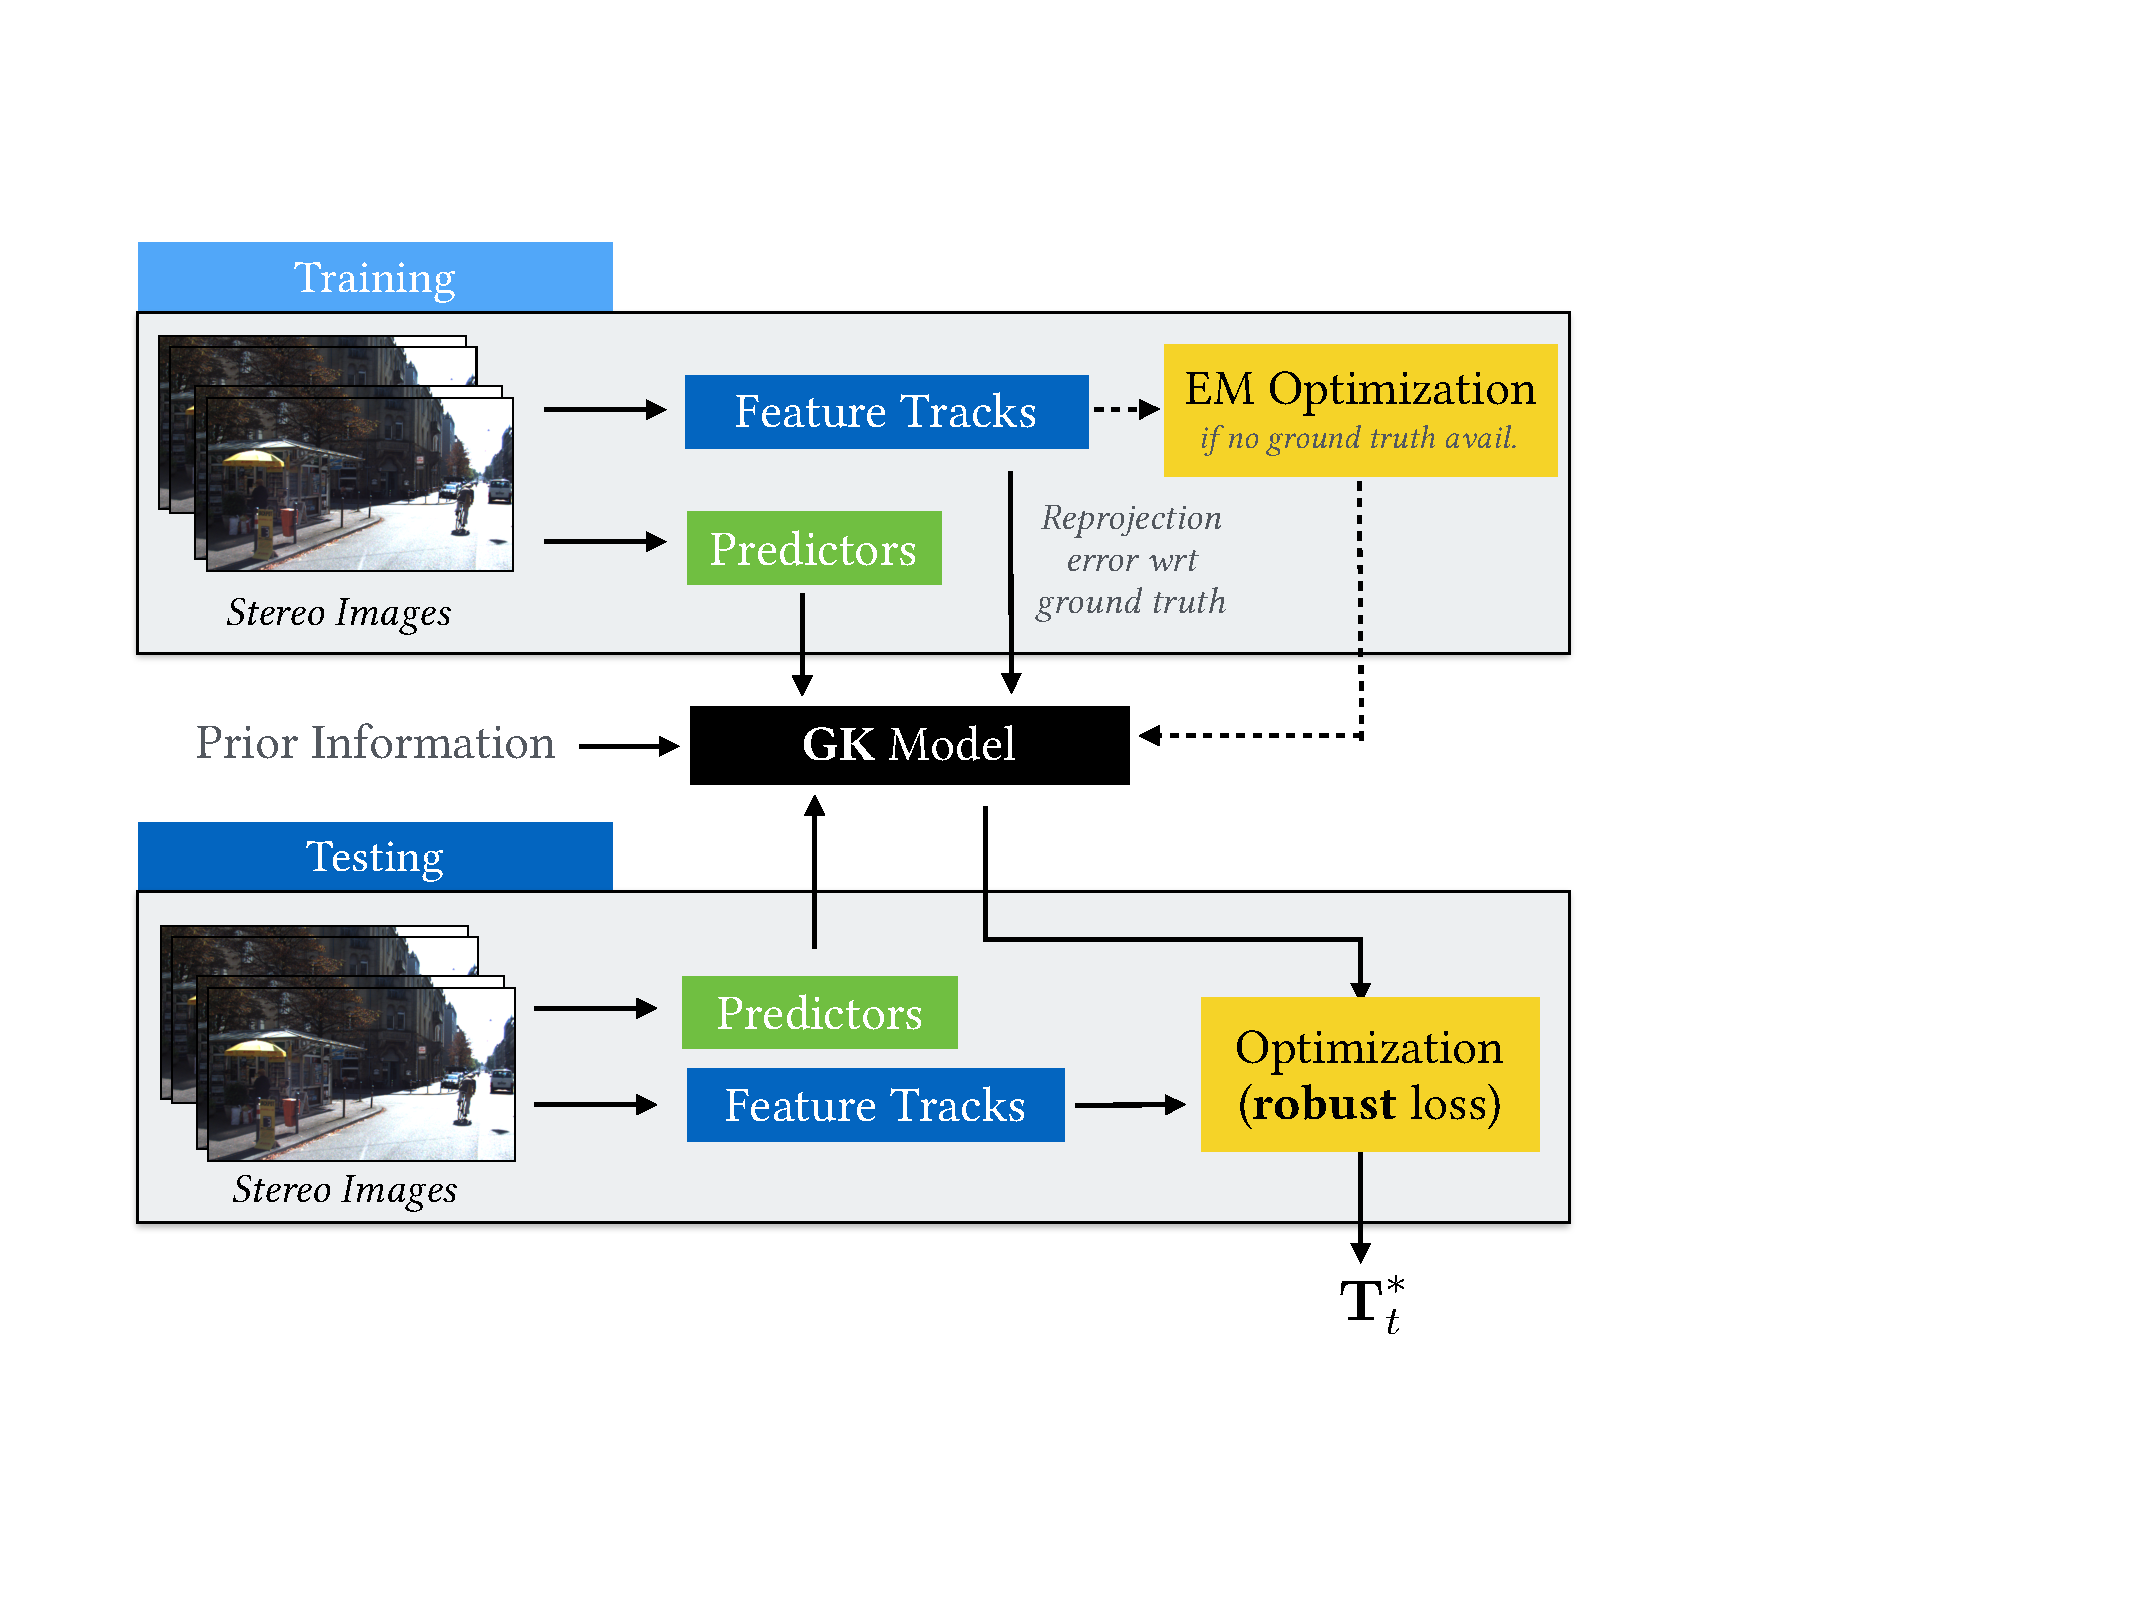
\includegraphics[width=0.48\columnwidth]{sun-bcnn/system_overview}
%      \caption{Our method uses a Bayesian Convolutional Neural Network (BCNN) to estimate the direction of the sun and to produce a principled uncertainty estimate for each prediction. We incorporate this \emph{virtual sun sensor} into a stereo visual odometry pipeline to reduce estimation error.}
%    \label{fig:sun-bcnn_system}
%\end{wrapfigure}

This accumulated error, or drift, can be limited by incorporating global information into the motion estimation problem.
This frequently takes the form of a globally consistent map, loop closure detection, or reliance on additional sensors such as GPS to make corrections to the estimated trajectory.
In many situations, however, a globally consistent map may be unavailable or prohibitively expensive to compute, loop closures may not occur, or GPS may be unavailable or inaccurate.
In such cases, it can be advantageous to rely on environmental cues such as the sun, which can easily provide global orientation information since it is readily detectable and its apparent motion in the sky is well described by ephemeris models.


\begin{figure}
    \centering
    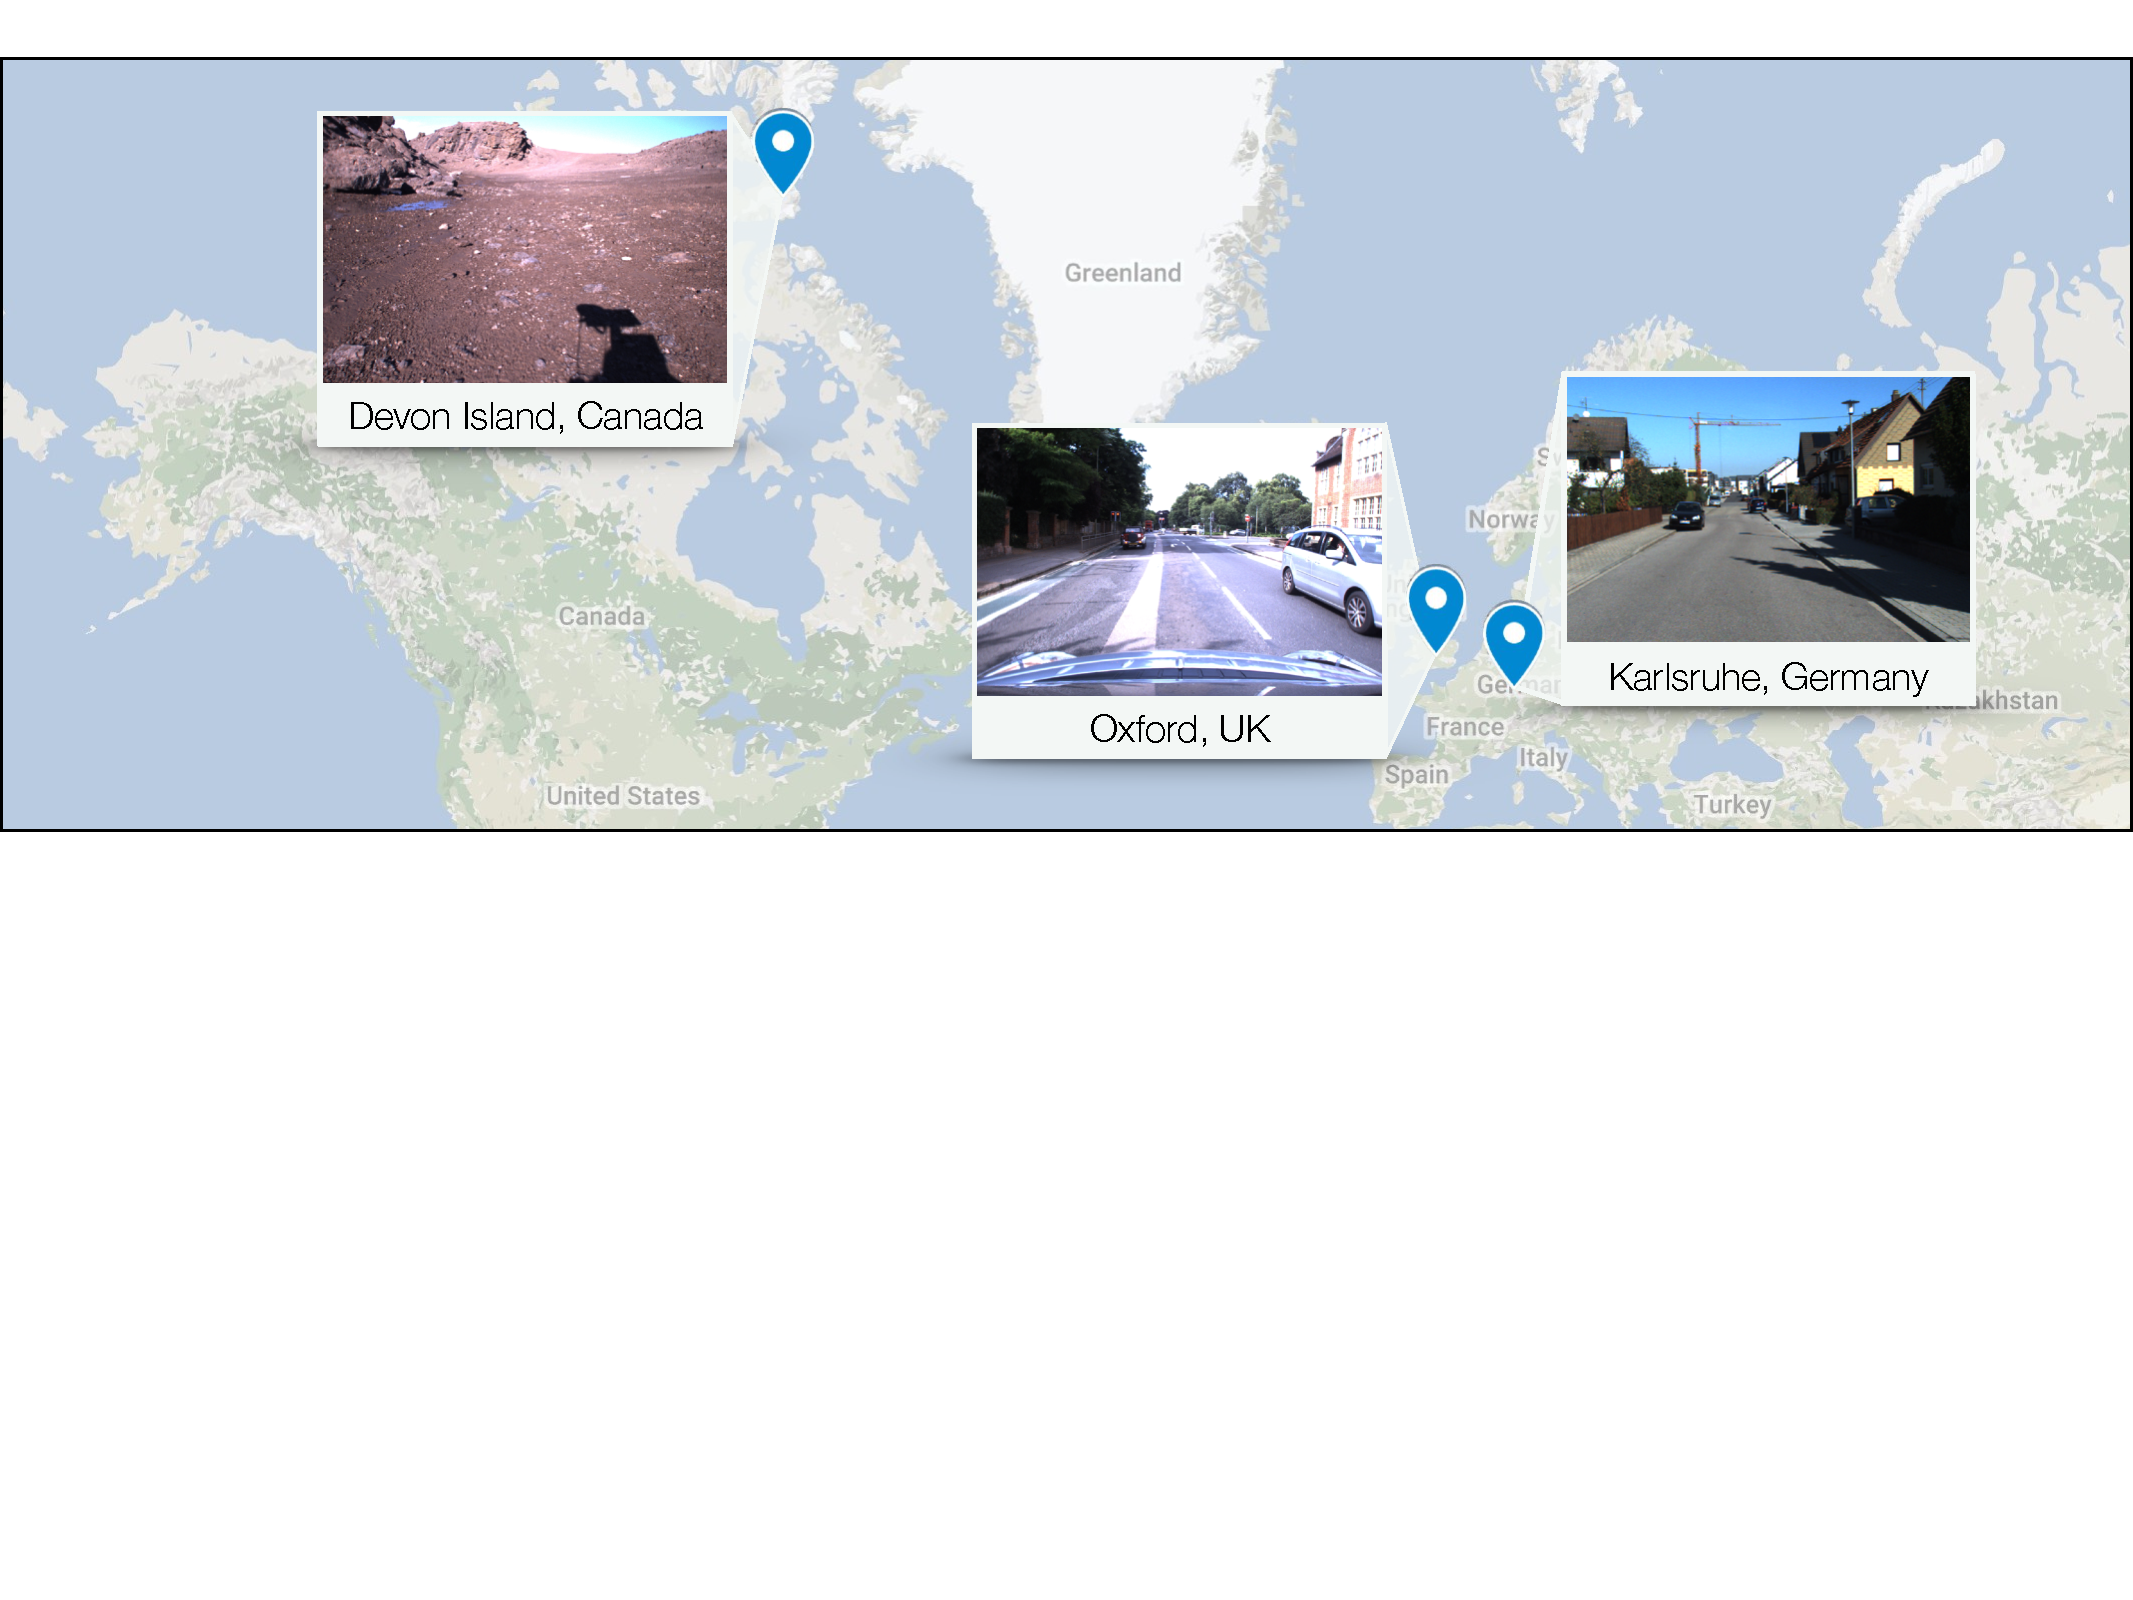
\includegraphics[width=0.98\textwidth]{sun-bcnn/all_datasets_gps}
    \caption{We train and test Sun-BCNN in a variety of environments ranging from urban driving in Europe to remote planetary analogue sites in the Canadian High Arctic. (Map data: Google, INEGI, ORION-ME.)}
    %\vspace{-0.4em}
    \label{fig:sun-bcnn_global-gps}
\end{figure}





For visual odometry (VO) in particular, the addition of global orientation information can limit the growth of drift error to be linear rather than superlinear with distance traveled \citep{Olson2003-ax}.

Sun-based orientation corrections have been successfully used in planetary analogue environments \citep{Furgale2011-zu,Lambert2012-sn} as well as on board the Mars Exploration Rovers (MERs) \citep{Eisenman2002-cg,Maimone2007-tc}.
In particular, \citet{Lambert2012-sn} showed that incorporating sun sensor and inclinometer measurements directly into the motion estimation pipeline (as opposed to periodically updating the vehicle heading, as in earlier work) can significantly reduce VO drift over long trajectories.


In this work, we seek to answer the question of whether similar reductions in VO drift can be obtained solely from the image stream already being used to compute VO.
The main idea here is that by reasoning over more than just the geometric information available from a standard RGB camera, we can improve existing VO techniques without needing to rely on a dedicated sun sensor or specially oriented camera.
In particular, we leverage recent advances in Bayesian Convolutional Neural Networks (BCNNs) to demonstrate how we can build and train a deep model capable of inferring the direction of the sun from a single RGB image. 
Moreover, we show that our network, dubbed Sun-BCNN, can produce a covariance estimate for each observation that obviates the need for a hand-tuned or empirically computed static covariance typically used for data fusion in a motion estimation pipeline. 




The remainder of this chapter begins with a discussion of related work, followed by an overview of the theory underlying BCNNs and a discussion of our model architecture, implementation, and training procedure.
We then outline our chosen visual odometry pipeline, which is based is an adapted version of the pipeline describe in \Cref{ch:vo}, and describe how observations of the sun can be incorporated directly into the motion estimation problem following the technique of \citet{Lambert2012-sn}.
Finally, we present several sets of experiments designed to test and validate both Sun-BCNN and our sun-aided VO pipeline in variety of environments.
These include experiments on 21.6~km of urban driving data from the KITTI odometry benchmark training set \citep{Geiger2013-ky}, as well as a further 10~km traverse through a planetary analogue site taken from the Devon Island Rover Navigation Dataset collected in a planetary analogue site in the Canadian High Arctic \citep{Furgale2012-kk}.
We investigate the possibility of model generalization between different cameras and environments, and further explore the sensitivity of Sun-BCNN to cloud cover during training and testing, using data from the Oxford Robotcar Dataset \citep{Maddern2016-ng}.
We also examine the impact of different methods for computing the mean and covariance of a norm-constrained vector on the accuracy and consistency of the estimated sun directions.

\section{Related Work}

%Visual odometry (VO), a technique to estimate the motion of a moving platform equipped with one or more cameras, has a rich history of research including a notable implementation onboard the Mars Exploration Rovers (MERs) \citep{Scaramuzza2011-qr}. 
%Modern approaches to VO can achieve estimation errors below 1\% of total distance traveled  \citep{Geiger2013-ky}. 
%To achieve such accurate and robust estimates, modern techniques use careful visual feature pruning \citep{Cvisic2015-mt}, adaptive robust methods  \citep{Alcantarilla2016-kv,Peretroukhin2016-om}, or operate directly on pixel intensities \citep{Engel2015-il}.

Independent of the type of estimator, VO exhibits superlinear error growth, and is particularly sensitive to errors in orientation \citep{Olson2003-ax, Cvisic2015-mt}. 
One way to reduce orientation error is to incorporate observations of a landmark whose position or direction in the navigation frame is known \emph{a priori}. 
The sun is an example of such a known directional landmark. 
Accordingly, hardware sun sensors have been used to improve the accuracy of VO in planetary analogue environments (e.g., the Sinclair Interplanetary SS-411 sun sensor used by \citet{Furgale2011-zu} and \citet{Lambert2012-sn}), while the MERs articulated their Pancam apparatus to directly image the sun~\citep{Maimone2007-tc,Eisenman2002-cg}. 
More recently, software-based alternatives have been developed that can estimate the direction of the sun from a single image, making sun-aided navigation possible without additional sensors or a specially-oriented camera \citep{2017_Clement_Improving}. 
Some of these methods have been based on hand-crafted illumination cues such as shadows and variation in sky brightness \citep{Lalonde2011-jw,2017_Clement_Improving}, while others have attempted to learn such cues from data using deep Convolutional Neural Networks (CNNs) \citep{Ma2016-at}.

Convolutional Neural Networks (CNNs) have been applied to a wide range of classification, segmentation, and learning tasks in computer vision \citep{LeCun2015-qf}. 
Recent work has shown that CNNs can learn orientation information directly from images by modifying the loss functions of existing discrete classification-based CNN architectures into continuous regression losses \citep{Ma2016-at, Kendall2015-ew, Kendall2016-zf}. 
Despite their success in improving prediction accuracy, most existing CNN-based models do not report uncertainty estimates, which are important in the context of data fusion.

For classification, it is possible to restrict CNN model outputs to a certain range (e.g., using a softmax function) and interpret these values as the model's confidence in its output. As \citet{Gal2016UncertaintyThesis} noted, however, this can be misleading because these  values can be unjustifiably large for test points far away from training data.  To address this, \citet{Gal2016-ny} showed that it is possible to achieve covariance outputs that better quantify model uncertainty for classification and regression tasks, with only minor modifications to existing CNN architectures. 
An early application of this uncertainty quantification was presented by \citet{Kendall2016-zf} who used it to improve their prior work \citep{Kendall2015-ew} on camera pose regression.

We build on on previous work by \citet{2017_Clement_Improving}, who demonstrated empirically that techniques for single-image sun estimation based on hand-crafted models \citep{Lalonde2011-jw} and Convolutional Neural Networks (CNNs) \citep{Ma2016-at} could be incorporated into a stereo visual odometry pipeline to reduce estimation error in the manner of \citet{Lambert2012-sn}.
We also build on the work of \citet{2017_Peretroukhin_Reducing}, who presented preliminary experimental results comparing Sun-BCNN against the method of \citet{Lalonde2011-jw} and its VO-informed variant \citep{2017_Clement_Improving} as well as the Sun-CNN of \citet{Ma2016-at} on the KITTI odometry benchmark \citep{Geiger2013-ky}, both in terms of raw measurement accuracy and in terms of their impact on VO accuracy.

While our method is similar in spirit to the work of \citet{Ma2016-at}, who built a CNN-based sun sensor as part of a relocalization pipeline, our model makes three important improvements: 1) in addition to a point estimate of the sun direction, we output a principled covariance estimate that is incorporated into our estimator; 2) we produce a full 3D sun direction estimate with azimuth and zenith angles that is better suited to 6-DOF robot pose estimation problems (as opposed to only the azimuth angle and 3-DOF estimator used by \citet{Ma2016-at}); and 3) we incorporate the sun direction covariance into a VO estimator that accounts for growth in pose uncertainty over time (unlike \citet{2017_Clement_Improving}). 
Furthermore, our Bayesian CNN includes a dropout layer after every convolutional and fully connected layer (as outlined by \citet{Gal2016-ny} but not done by \citet{Kendall2016-zf}).


\section{Sun-Aided Stereo Visual Odometry} 
\label{sec:sun_bcnn-stereo-vo}
For this work, we adopt a sliding window sparse stereo VO technique (derived from the frame-to-frame pipeline described in \Cref{ch:vo}) that has been used in a number of successful mobile robotics applications \citep{Cheng2006-nl,Furgale2010-to,Geiger2011-xe,Kelly2008-mh}.
Our task is to estimate a window of $\LieGroupSE{3}$ poses $\Set{\Transform_{k_1,0}, \Transform_{k_1+1,0}, \dots, \Transform_{k_2-1, 0}, \Transform_{k_2, 0}}$ expressed in a base coordinate frame $\CoordinateFrame{0}$, given a prior estimate of the transformation $\Transform_{k_1,0}$.
We accomplish this by tracking keypoints across pairs of stereo images and computing an initial guess for each pose in the window using frame-to-frame point cloud alignment, which we then refine by solving a local bundle adjustment problem over the window.
In our experiments we choose a window size of two, which we observed to provide good VO accuracy at low computational cost. 
We select the initial pose $\Transform_{1,0}$ to be the first GPS ground truth pose such that $\CoordinateFrame{0}$ is a local East-North-Up (ENU) coordinate system with its origin at the first GPS position.

\subsection{Observation Model}
We assume that incoming stereo images have been undistorted and rectified in a pre-processing step, and model the stereo camera as a pair of perfect pinhole cameras with focal lengths $f_u, f_v$ and principal points $\left(c_u,c_v\right)$, separated by a fixed and known baseline $b$ (see \Cref{sec:vo_data_extraction}).

If we take $\Keypoint_0^j$ to be the homogeneous 3D coordinates of keypoint $j$, expressed in our chosen base frame $\CoordinateFrame{0}$, we can transform the keypoint into the camera frame at pose $k$ to obtain $\Keypoint_k^j = \Transform_{k,0}\Keypoint_0^j = \Transpose{\bbm \KeypointComponent_{k,x}^j & \KeypointComponent_{k,y}^j & \KeypointComponent_{k,z}^j & 1 \ebm}$. Our observation model $\Vector{g}\left(\cdot\right)$ (defined with disparity, unlike the function $\Vector{f}(\cdot)$ in \Cref{sec:vo_data_extraction}) can then be formulated as
\begin{align} \label{eq:cam_model}
    \Vector{y}_{k,j} &= \CameraModel{\Keypoint_k^j}
%                    = \CameraModel{\Transform_{k,0} \Keypoint_0^j}
                    = \bbm u \\ v \T \\ d \T \ebm 
                    = \bbm 
			   		    f_u \KeypointComponent_{k,x}^j / \KeypointComponent_{k,z}^j + c_u \\
			   		    f_v \KeypointComponent_{k,y}^j / \KeypointComponent_{k,z}^j + c_v \T \\
			   		    f_u b / \KeypointComponent_{k,z}^j  \T
			         \ebm,
\end{align}
where $\left(u,v\right)$ are the keypoint coordinates in the left image and $d$ is the disparity in pixels.

\subsection{Sliding Window Bundle Adjustment}
Like with PROBE, we use the open-source \texttt{viso2} package \citep{Geiger2011-xe} to detect and track keypoints between stereo image pairs.
Based on these keypoint tracks, a three-point Random Sample Consensus (RANSAC) algorithm \citep{fischler1981random} generates an initial guess of the interframe motion and rejects outlier keypoint tracks by thresholding their reprojection error.
We compound these pose-to-pose transformation estimates through our chosen window and refine them using a local bundle adjustment, which we solve using the nonlinear least-squares solver Ceres \citep{ceres-solver}.
The objective function to be minimized can be written as
\begin{equation} \label{eq:cost_function}
    \BACost = \BACost_\text{reprojection} + \BACost_\text{prior},
\end{equation}
where
\begin{equation} \label{eq:reprojection_cost}
	\BACost_\text{reprojection} = \sum_{k=k_1}^{k_2} \sum_{j=1}^J \Transpose{\Error}_{\CameraObservation_{k,j}} \Covariance^{-1}_{\CameraObservation_{k,j}} \Error_{\CameraObservation_{k,j}}
\end{equation}
and 
\begin{equation} \label{eq:prior_cost}
	\BACost_\text{prior} = \Transpose{\Error}_{\Estimate{\Transform}_{k_1,0}} \Covariance^{-1}_{\Estimate{\Transform}_{k_1,0}} \Error_{\Estimate{\Transform}_{k_1,0}}.
\end{equation}

The quantity $\Error_{\CameraObservation_{k,j}} = \Estimate{\CameraObservation}_{k,j} - \CameraObservation_{k,j}$ represents the reprojection error of keypoint $j$ for camera pose $k$, with $\Covariance_{\CameraObservation_{k,j}}$ being the covariance of these errors.
The predicted measurements are given by $\Estimate{\CameraObservation}_{k,j} = \CameraModel{\Estimate{\Transform}_{k,0} \Estimate{\Keypoint}^j_{0}}$, where $\Estimate{\Transform}_{k,0}$ and $\Estimate{\Keypoint}^j_{0}$ are the estimated poses and keypoint positions in base frame $\CoordinateFrame{0}$.

The cost term $\BACost_\text{prior}$ imposes a normally distributed prior $\Prior{\Transform}_{k_1,0}$ on the first pose in the current window, based on the estimate of this pose in the previous window.
The error in the current estimate $\Estimate{\Transform}_{k_1,0}$ of this pose compared to the prior can be computed via the $\LieGroupSE{3}$ matrix logarithm as $\Error_{\Prior{\Transform}_{k_1,0}} = \log \left( \Prior{\Transform}_{k_1,0}^{-1} \Estimate{\Transform}_{k_1,0} \right)^\vee \in \mathbb{R}^6$.
The $6 \times 6$ matrix $\Covariance_{\Prior{\Transform}_{k_1,0}}$ is the covariance associated with $\Prior{\Transform}_{k_1,0}$ in its local tangent space, and is obtained as part of the previous window's bundle adjustment solution.
This prior term allows consecutive windows of pose estimates to be combined in a principled way that appropriately propagates global pose uncertainty from window to window, which is essential in the context of optimal data fusion.

\section{Orientation Correction}
In order to combat drift in the VO estimate produced by accumulated orientation error, we adopt the technique of \citet{Lambert2012-sn} to incorporate absolute orientation information from the sun directly into the estimation problem.
We assume the initial camera pose and its timestamp are available from GPS and use them to determine the global direction of the sun $\Vector{s}_0$, expressed as a 3D unit vector, from ephemeris data.
We define the world frame $\CoordinateFrame{0}$ to be a local ENU coordinate system with the initial GPS position as its origin.
At each timestep we update $\SunDirection_0$ by querying the ephemeris model using the current timestamp and the initial camera pose, allowing our model to account for the apparent motion of the sun over long trajectories.

By transforming the global sun direction into each camera frame $\CoordinateFrame{k}$ in the window, we obtain predicted sun directions $\Estimate{\SunDirection}_k = \Estimate{\Transform}_{k,0} \SunDirection_0$, where $\Estimate{\Transform}_{k,0}$ is the current estimate of camera pose $k$ in the base frame. 
We compare the predicted and estimated sun directions to introduce an additional error term into the bundle adjustment cost function (cf. \Cref{eq:cost_function}):
\begin{equation} \label{eq:cost_function_with_sun}
    \BACost = \BACost_\text{reprojection} + \BACost_\text{prior} + \BACost_\text{sun},
\end{equation}
where 
\begin{equation} \label{eq:sun_cost}
	\BACost_\text{sun} = \sum_{k=k_1}^{k_2} \Transpose{\Error}_{\SunDirection_k} \Covariance^{-1}_{\SunDirection_k} \Error_{\SunDirection_k},
\end{equation}
and $\BACost_\text{reprojection}$ and $\BACost_\text{prior}$ are defined in \Cref{eq:reprojection_cost,eq:prior_cost}, respectively.
This additional term constrains the orientation of the camera, which helps limit drift in the VO result due to orientation error \citep{Lambert2012-sn}.

Since $\SunDirection_k$ is constrained to be unit length, there are only two underlying degrees of freedom.
We therefore define $\Vector{f}\left(\cdot\right)$ to be a function that transforms a 3D unit vector in camera frame $\CoordinateFrame{k}$ to a zenith-azimuth parametrization:
\begin{equation} \label{eq:vec-to-az-zen}
	\bbm \theta \\ \phi \ebm
    = \Vector{f} \left( \SunDirection_k \right)
    = \bbm \text{acos}\left( -\SunDirectionComponent_{k,y} \right) \\ \text{atan2}\left(\SunDirectionComponent_{k,x}, \SunDirectionComponent_{k,z} \right) \ebm
\end{equation}
where $\SunDirection_k = \Transpose{\bbm \SunDirectionComponent_{k,x} & \SunDirectionComponent_{k,y} & \SunDirectionComponent_{k,z} \ebm}$.
We can then define the term $\Error_{\SunDirection_k} = \Vector{f}\left(\Estimate{\SunDirection}_k\right) - \Vector{f}\left(\SunDirection_k\right)$ to be the error in the predicted sun direction, expressed in azimuth-zenith coordinates, and $\Covariance_{\SunDirection_k}$ to be the covariance of these errors.
While $\Covariance_{\SunDirection_k}$ would generally be treated as an empirically determined static covariance, in our approach we use the per-observation covariance computed using \Cref{eq:bcnn_covar}, which allows us to weight each observation individually according to a measure of its intrinsic quality.
In practice, we also attempt to mitigate the effect of outlier sun predictions by applying a robust Huber loss to the sun measurements in our optimizer.


\section{Bayesian Convolutional Neural Networks}

Recall from \Cref{section:math_dl_practical} that dropout (\Cref{fig:sun-bcnn_fcn_dropout}) is a stochastic regularization technique that was originally designed to improve the generalization performance of deep networks. Dropout works by randomly `turning off' certain inputs of layers to simulate an ensemble of smaller networks during training. \cite{Gal2016CNN} identified a link between applying dropout at test-time given a network trained with dropout (through a technique called \textit{Monte Carlo dropout}, or \textit{MC dropout}) and approximate variational inference for a particular type of Bayesian Neural Network. In this work, we leverage this insight to build a Bayesian Convolutional Neural Network through MC dropout. To elucidate the intuition behind this technique, we first review variational inference and then outline its connection to the technique of dropout. 


\begin{figure}
\centering
\begin{subfigure}{0.45\textwidth}
	\centering
    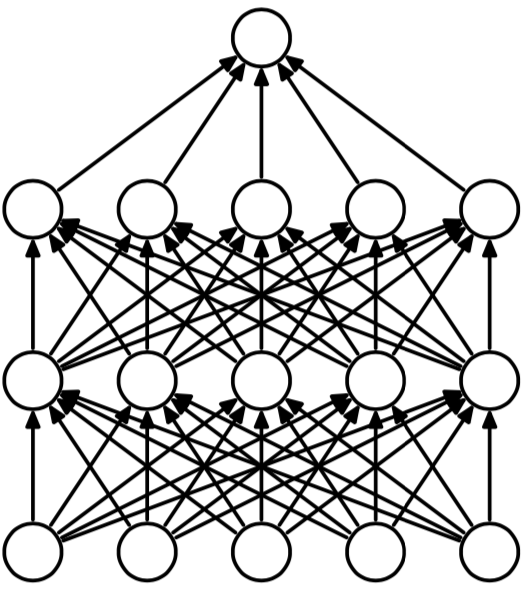
\includegraphics[width=0.8\textwidth]{sun-bcnn/dropout_fcn}
    \caption{Standard fully-connected neural network.}
\end{subfigure}
~
\begin{subfigure}{0.45\textwidth}
	\centering
    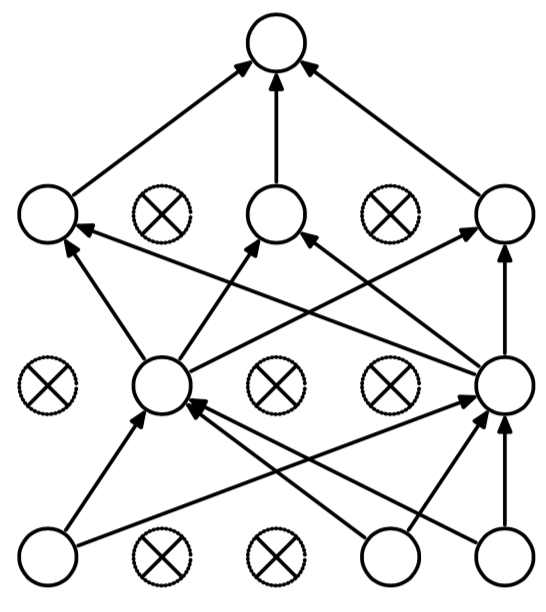
\includegraphics[width=0.8\textwidth]{sun-bcnn/dropout_fcnwdrop}
    \caption{A neural network with dropout applied.}
\end{subfigure}
\caption{The technique of \textit{dropout} stochastically removes the contribution of certain neurons to regularize learning. Figures	 from \cite{srivastava_dropout_2014}.}
\label{fig:sun-bcnn_fcn_dropout}
\end{figure}

\subsection{Bayesian Modelling and Variational Inference}

Consider the goal of generating a function $f(\Vector{x}; \GenericParameters)$ that maps inputs $\Vector{x}$ to outputs $\Vector{y}$ as a function of parameters $\GenericParameters$. Recall from \Cref{ch:probe} that in Bayesian inference we define a \textit{prior} on the space of parameters $p(\GenericParameters)$ and a \textit{likelihood function} that defines how likely we are to observe $\Vector{y}$ given an input $\Vector{x}$ and parameters $\GenericParameters$, $p(\Vector{y} | \Vector{x}, \GenericParameters)$. For example, in regression problems, we often define the Gaussian likelihood
\begin{equation}
	p(\Vector{y} | \Vector{x}, \GenericParameters) = \NormalDistribution(f(\Vector{x}; \GenericParameters),\tau^{-1}\IdentityMatrix)
\end{equation}
where $\tau$ is a model \textit{precision}. Given a dataset $\mathcal{D} = \{\Matrix{X}, \Matrix{Y}\} = \{\{\Vector{x}_1, ... \Vector{x}_N\},\{\Vector{y}_1, ..., \Vector{y}_N)\} \}$, the Bayesian formulation seeks a posterior over the parameters $\GenericParameters$:
\begin{equation}
\label{eq:sun_bcnn_param_posterior}
	p(\GenericParameters | \mathcal{D}) = \frac{p(\Matrix{Y}|\Matrix{X}, \GenericParameters) p(\GenericParameters)}{p(\Matrix{Y} | \Matrix{X})}
\end{equation}
where we may think of this posterior as evaluating the sentence `the likelihood of the observed outputs given a particular set of parameters (weighted by a prior) compared to how likely they are in general'. This latter `in general' quantity is the marginal likelihood (also known as the model \textit{evidence}) over the space of parameters,
\begin{equation}
	p(\Matrix{Y} | \Matrix{X}) = \int_{\GenericParameters}  p(\Matrix{Y} | \Matrix{X}, \GenericParameters) p(\GenericParameters) d\GenericParameters.
\end{equation}
For a given test input $\Vector{x}^*$, we can then \textit{infer} a predictive distribution over the space of outputs by integrating over the posterior of model parameters:
\begin{equation}
	p(\Vector{y}^* | \Vector{x}^*, \mathcal{D}) = \int_{\GenericParameters}  p(\Vector{y}^* | \Vector{x}^*, \GenericParameters) p(\GenericParameters | \mathcal{D}) d\GenericParameters.
\end{equation}
For most problems, evaluating the posterior (\Cref{eq:sun_bcnn_param_posterior}) analytically is not feasible. In such cases, we can turn to the technique of \textit{variational inference} \citep{Gal2016UncertaintyThesis}.

\subsubsection{Variational Inference}
In variational inference, we define a simpler variational density $q(\GenericParameters; \Vector{\theta})$ based on the auxiliary parameters $\Vector{\theta}$. We then seek to minimize the Kullback-Leibler (KL) divergence \citep{kullback1951information} between $q(\GenericParameters; \Vector{\theta})$ and the true posterior $p(\GenericParameters | \mathcal{D})$:
\begin{equation}
\label{eq:sun_bcnn_KL}
	\Vector{\theta}^* = \ArgMin{\Vector{\theta}}\text{KL}(q(\GenericParameters; \Vector{\theta}) || p(\GenericParameters | \mathcal{D})) = \ArgMin{\Vector{\theta}} \int q(\GenericParameters; \Vector{\theta}) \log \frac{q(\GenericParameters; \Vector{\theta})}{p(\GenericParameters | \mathcal{D})} d \GenericParameters,
\end{equation}
which then allows us to compute the approximate predictive distribution as
\begin{equation}
	p(\Vector{y}^* | \Vector{x}^*, \mathcal{D}) \approx \int_{\GenericParameters}  p(\Vector{y}^* | \Vector{x}^*, \GenericParameters) q(\GenericParameters; \Vector{\theta}^*) d\GenericParameters.
\end{equation}
One can show (see, for example, \cite{Gal2016UncertaintyThesis}) that minimizing KL divergence (\Cref{eq:sun_bcnn_KL}) is the same as maximizing the evidence lower bound (ELBO)\footnote{KL divergence and the ELBO differ by a constant that is not dependent on the auxiliary variables.} 
\begin{equation}
\label{eq:sun_bcnn_ELBO}
	\Vector{\theta}^* = \ArgMax{\Vector{\theta}} -\mathcal{L}_{\text{ELBO}} = \ArgMax{\Vector{\theta}} \int_{\GenericParameters}  \log p(\Matrix{Y} | \Matrix{X}, \GenericParameters)  q(\GenericParameters; \Vector{\theta}) d\GenericParameters -  \text{KL}(q(\GenericParameters; \Vector{\theta}) ~ || ~ p(\GenericParameters)).
\end{equation}
Intuitively, maximizing the first term above (referred to as the expected log likelihood) ensures that $q(\GenericParameters; \Vector{\theta})$ explains the dataset well, while minimizing the latter term regularizes the optimization so that $q(\GenericParameters; \Vector{\theta})$ does not stray too far away from a prior.




\subsection{Monte Carlo Dropout as Approximate Variational Inference}
A key insight of \cite{Gal2016UncertaintyThesis, Gal2016-ny} was that the training objective of a neural network with dropout resembles the ELBO optimization of \Cref{eq:sun_bcnn_ELBO} with a careful choice of $q(\GenericParameters; \Vector{\theta})$.
Namely, consider training a neural network with dropout and with another form of regularization called \textit{weight decay} (which penalizes large weight magnitudes). The loss function for supervised training in this scenario can be written as
\begin{equation}
\label{eq:sun_bcnn_dropout_obj}
\mathcal{L}_{\text{dropout}}(\GenericParameters) = \underbrace{\frac{1}{N} \sum_{i=1}^N \mathcal{E}(\Vector{y}_i, \tilde{\Vector{y}}_i)}_{\text{error function}} + \underbrace{\lambda \sum_{\ell=1}^L	\left( \Norm{\Matrix{W}_\ell}_2^2 +  \Norm{\Vector{b}_\ell}_2^2\right)}_{\text{weight decay}},
\end{equation}
where $\Vector{y}_i$ is the target output, $\lambda$ is a scalar weight decay hyper-parameter, and $\tilde{\Vector{y}}_i = NN(\Vector{x}_i)$ is a stochastic sample of the network output with dropout applied. Now if we define $q(\GenericParameters)$ to be a \textit{Bernoulli variational distribution}  over the network parameters as the re-parametrized density,
\begin{align}
	q(\GenericParameters; \Vector{\theta}) &= \{\text{diag} (\{ \epsilon_{i\ell} \}) \Matrix{W}_\ell, \Vector{b}_\ell\}_{\ell=1}^L \\
	\epsilon_{i\ell} &\sim \text{Bernoulli}(p) 
\end{align}
where the auxiliary variables become the network parameters themselves, $\Vector{\theta} = \{\Matrix{W}_\ell, \Vector{b}_\ell\}_{\ell=1}^L$. We can show an equivalence between optimizing the variational inference ELBO loss function,
\begin{align}
\mathcal{L}_{\text{ELBO}}(\Vector{\theta}) &= -\int_{\GenericParameters}  \log p(\Matrix{Y} | \Matrix{X}, \GenericParameters)  q(\GenericParameters; \Vector{\theta}) d\GenericParameters +  \text{KL}(q(\GenericParameters; \Vector{\theta}) ~ || ~ p(\GenericParameters))\\
&= - \sum_{i=1}^N \int_{\GenericParameters}  \log p(\Vector{y}_i | \Vector{x}_i, \GenericParameters)  q(\GenericParameters; \Vector{\theta}) d\GenericParameters + \text{KL}(q(\GenericParameters; \Vector{\theta}) ~ || ~ p(\GenericParameters))
\end{align}
and optimizing \Cref{eq:sun_bcnn_dropout_obj} above as follows. First, the first term above can be approximated through Monte Carlo integration with a single sample\footnote{In practice, stochastic gradient descent will select a mini-batch of these samples to give an unbiased estimate.} $\tilde{\GenericParameters}$ of $q(\GenericParameters; \Vector{\theta})$ such that, 
\begin{align}
	&= - \sum_{i=1}^N \log p(\Vector{y}_i | \Vector{x}_i, \tilde{\GenericParameters})  + \text{KL}(q(\GenericParameters; \Vector{\theta}) ~ || ~ p(\GenericParameters)).
\end{align}
Second, it is possible to show that there exist a Gaussian prior $p(\GenericParameters)$ such that the condition (Eq. 3.12, \cite{Gal2016UncertaintyThesis})
\begin{align}
\PartialDerivative{\text{KL}(q(\GenericParameters; \Vector{\theta}) ~ || ~ p(\GenericParameters))}{\Vector{\theta}} \approx \PartialDerivative{\lambda \sum_{\ell=1}^L	\left( \Norm{\Matrix{W}_\ell}_2^2 +  \Norm{\Vector{b}_\ell}_2^2\right)}{\Vector{\theta}}	
\end{align}
holds. Finally, if we interpret $-\log p(\Vector{y}_i | \Vector{x}_i, \tilde{\GenericParameters})$ as $\mathcal{E}(\Vector{y}_i, \tilde{\Vector{y}}_i)$ then it follows that
\begin{align}
\PartialDerivative{\mathcal{L}_{\text{ELBO}}}{\Vector{\theta}} \propto \PartialDerivative{\mathcal{L}_{\text{Dropout}}}{\Vector{\theta}}
\end{align} where the proportional constant can be written down analytically \citep{Gal2016UncertaintyThesis}. Thus the two objectives result in the same optimal parameters!
\subsubsection{Computing Moments}
The results above indicate that, once trained, a neural network with dropout gives us access to a predictive distribution over outputs $\Vector{y}$. An unbiased estimator for its mean and covariance are given by applying dropout at test time and computing statistics over $T$ samples:
\begin{equation}
\label{eq:sun_bcnn_mc_dropout_mean}
	\Expectation{\Vector{y}^*} = \frac{1}{T} \sum_{t=1}^T \tilde{\Vector{y}}^*_t,
\end{equation}
where $\tilde{\Vector{y}}^*_t = NN(\Vector{x}^*; \tilde{\GenericParameters}_t)$ and
\begin{equation}
\label{eq:sun_bcnn_mc_dropout_variance}
	\text{Var}(\Vector{y}^*) = \tau^{-1} \IdentityMatrix +  \frac{1}{T} \sum_{t=1}^T \tilde{\Vector{y}}^*_t (\tilde{\Vector{y}}^*_t)^T - \Expectation{\Vector{y}^*} \Expectation{\Vector{y}^*}^T,
\end{equation}
where the precision $\tau$ defines the likelihood 
\begin{equation}
	p(\Vector{y} | \Vector{x}, \GenericParameters) = \NormalDistribution(NN(\Vector{x}; \GenericParameters),\tau^{-1}\IdentityMatrix)	
\end{equation}
and can be alternatively modelled as
\begin{equation}
	\tau = \frac{l^2 (1 - p)}{2N\lambda},
\end{equation} 
where $l$ defines a characteristic length scale \citep{Gal2016UncertaintyThesis}. This test-time stochastic sampling through dropout is referred to as Monte Carlo dropout.

\subsection{Extension to Convolutional Neural Networks}
Although the derivation is more tedious, \cite{Gal2016UncertaintyThesis,Gal2016CNN} show that the same approximate variational inference can be carried out for convolutional neural networks by applying dropout after every convolution (and before pooling) during training and using MC dropout during testing.



\section{Indirect Sun Detection using a Bayesian Convolutional Neural Network} \label{sec:sun-bcnn}

\begin{figure}
    \centering
    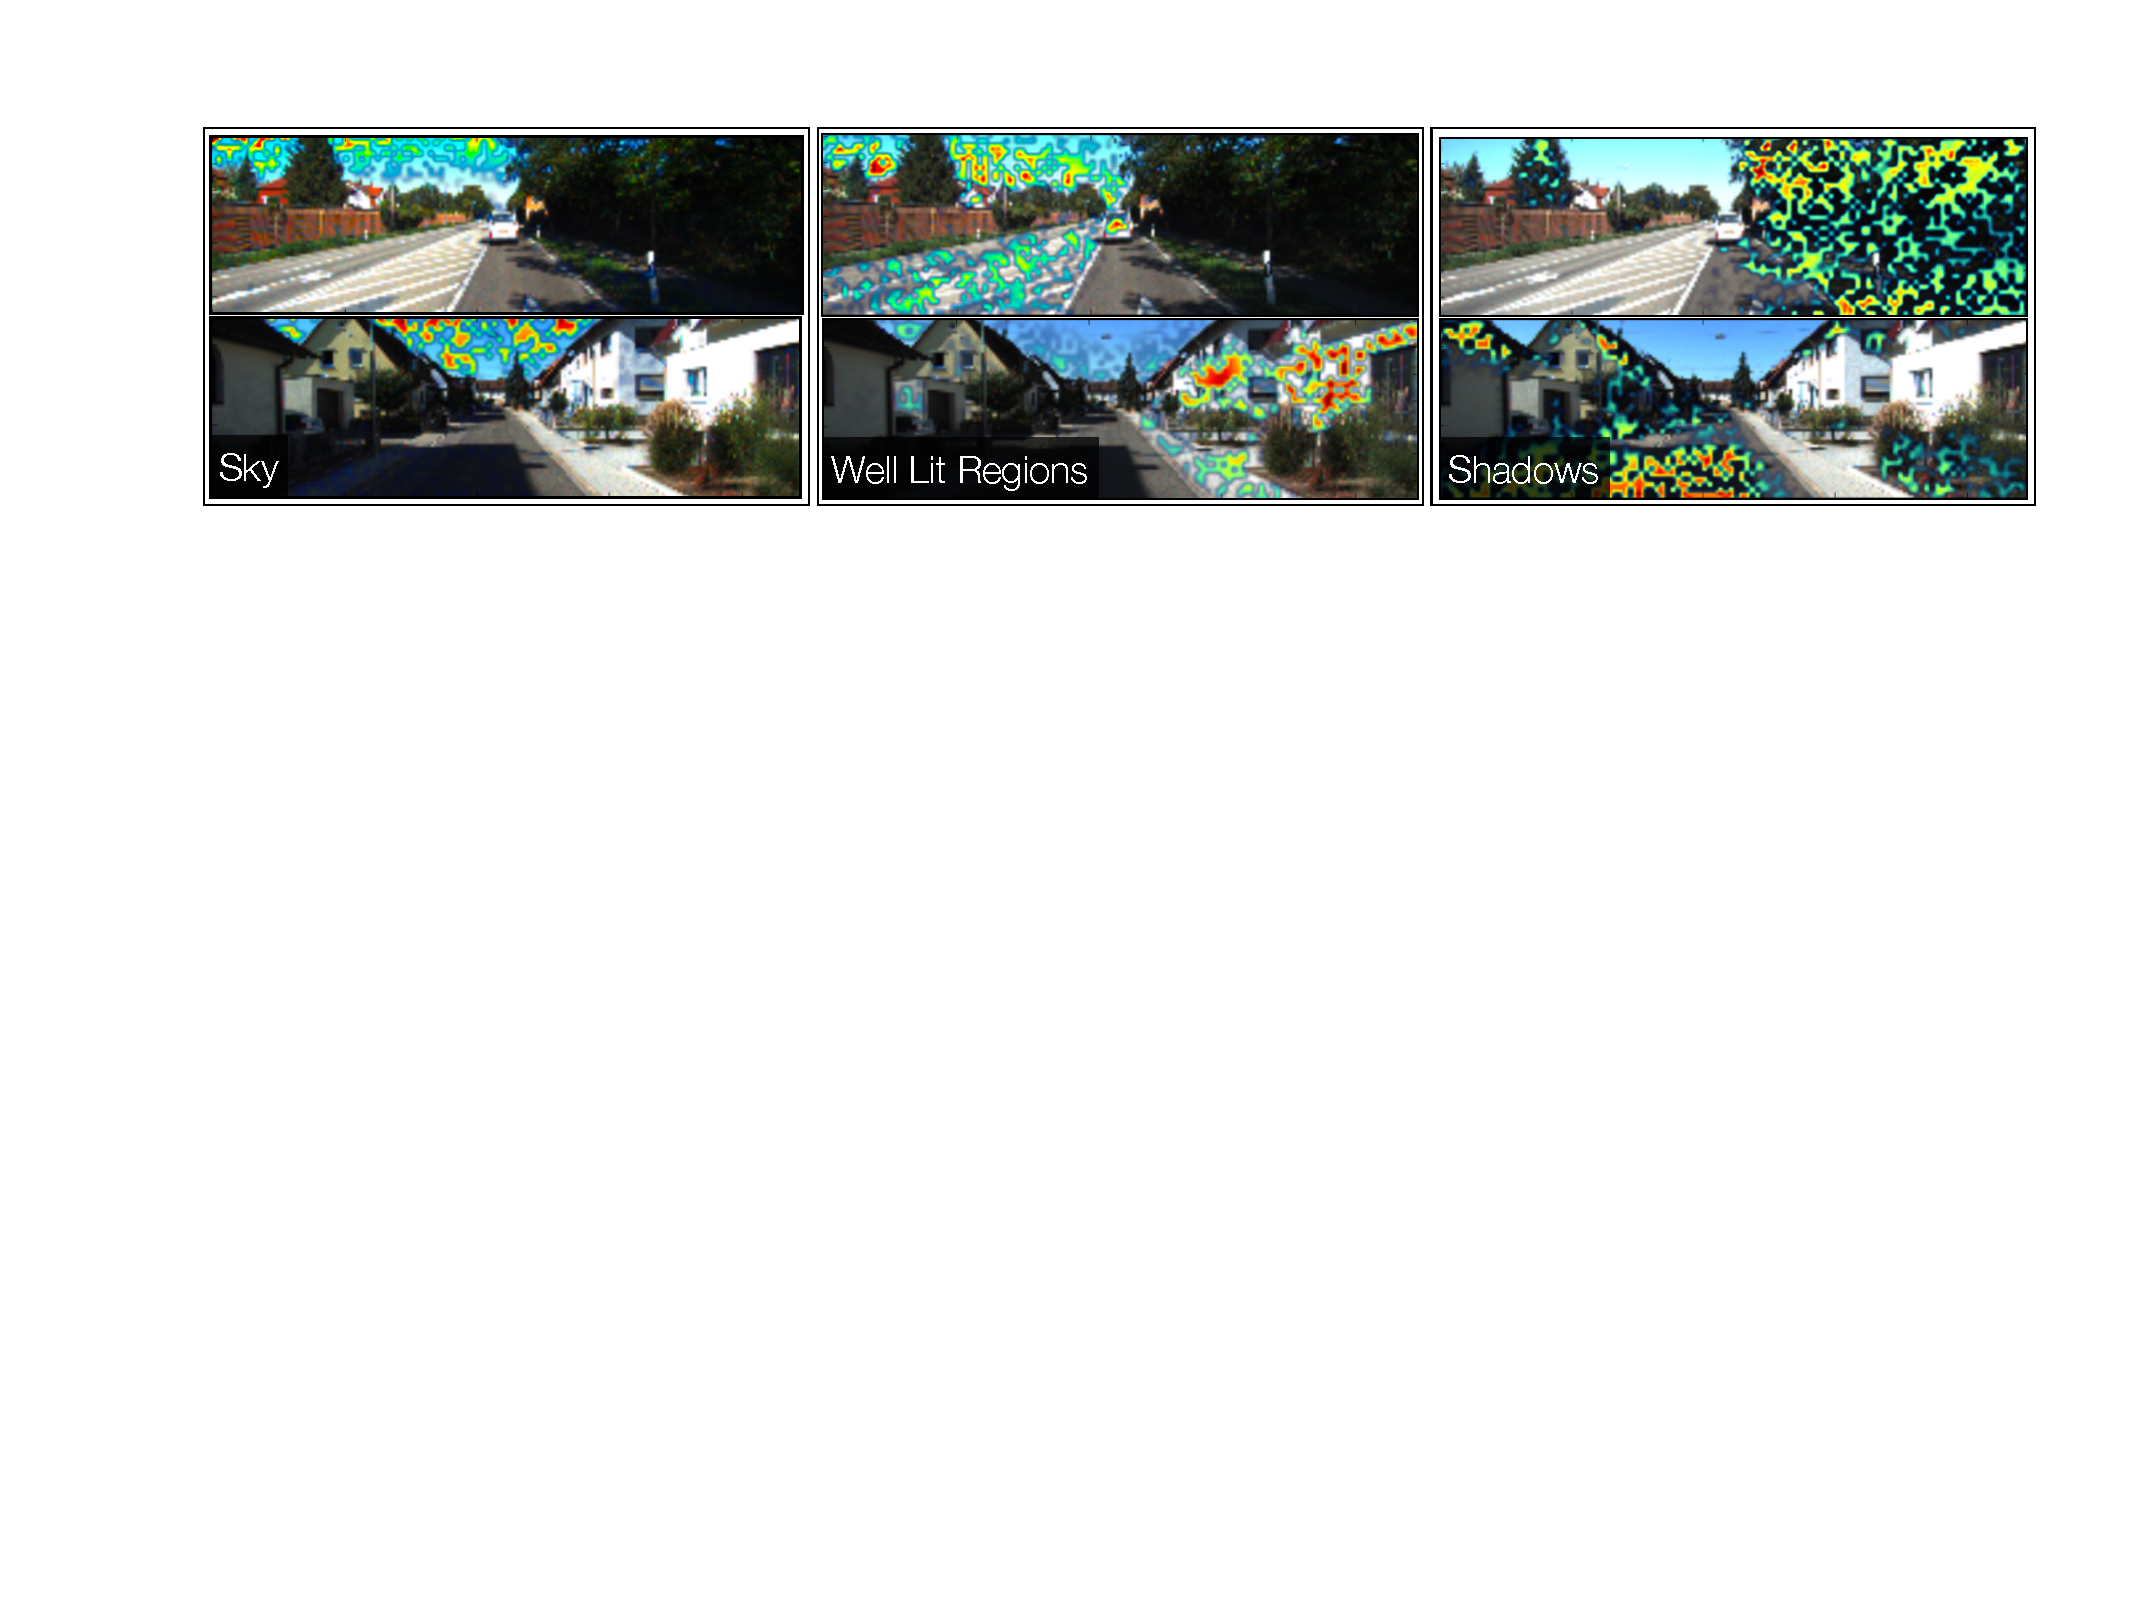
\includegraphics[width=0.98\textwidth]{sun-bcnn/kitti_activations_horiz}
    \caption{Three \texttt{conv1} layer activation maps superimposed on two images from the KITTI odometry benchmark \citep{Geiger2013-ky} \texttt{00} and \texttt{04} for three selected filters. Each filter picks out salient parts of the image that aid in sun direction inference.}
%      \vspace{-0.5em}
    \label{fig:sun-bcnn_kitti_cnn_activations}
\end{figure}

Leveraging the work of \cite{Gal2016CNN}, we apply MC dropout to a Convolutional Neural Network (CNN) (approximating a BCNN, or Bayesian CNNN) to infer the direction of the sun and an associated uncertainty, and refer to our model as Sun-BCNN. 
We motivate the choice of a deep model through the empirical findings of \citet{2017_Clement_Improving} and \citet{Ma2016-at}, who demonstrated that a CNN-based sun detector can substantially outperform hand-crafted models such as that of \citet{Lalonde2011-jw} both in terms of measurement accuracy and in its application to a VO task.

We choose a deep neural network structure based on GoogLeNet \citep{Szegedy2015-uw} due to its use in past work that adapted it for orientation regression \citep{Kendall2016-zf,Kendall2015-ew}. 
Unlike \citet{Ma2016-at}, we choose to transfer weights trained on the MIT Places dataset \citep{zhou2014MITPlaces} rather than ImageNet \citep{deng2009imagenet}.
We believe the MIT Places dataset is a more appropriate starting point for localization tasks than ImageNet since it includes outdoor scenes and is concerned with classifying physical locations rather than objects.

\subsection{Cost Function}
We train Sun-BCNN by minimizing the cosine distance between the unit-norm target sun direction vector $\SunDirection_k$  and the predicted unit-norm sun direction vector $\Estimate{\SunDirection}_k$, where $k$ indexes the images in the training set:
\begin{equation}
	\CNNLoss{\Estimate{\SunDirection}_k} = 1 - (\Estimate{\SunDirection}_k \cdot \SunDirection_k).
	\label{eq:cnn_loss}
\end{equation}
Note that in our implementation, we do not formulate the cosine distance loss explicitly, but instead minimize half the square of the tip-to-tip Euclidian distance between $\SunDirection_k$ and $\Estimate{\SunDirection}_k$, which is equivalent to \Cref{eq:cnn_loss} since both vectors have unit length:
\begin{align*}
 	\frac{1}{2} \Norm{\Estimate{\SunDirection}_k  - \SunDirection_k}^2 &= \frac{1}{2} \left( \Norm{\Estimate{\SunDirection}_k}^2 + \Norm{\SunDirection_k}^2 - 2 (\Estimate{\SunDirection}_k \cdot \SunDirection_k) \right) \\
 		&= 1 - (\Estimate{\SunDirection}_k \cdot \SunDirection_k) \\
 		&= \CNNLoss{\Estimate{\SunDirection}_k}.
\end{align*}
We ensure that our network output, $\Estimate{\SunDirection}_k$, has a unit norm by appending a normalization layer to the network.

\subsection{Uncertainty Estimation}
Using our notation for sun direction, we obtain the first two moments of the predictive distribution from our BCNN as (c.f. \Cref{eq:sun_bcnn_mc_dropout_mean,eq:sun_bcnn_mc_dropout_variance}):
\begin{align}
\label{eq:sun_direction_mean}
\Expectation{\Optimal{\Estimate{\SunDirection}}}_k &= \Optimal{\Estimate{\Mean{\SunDirection}}}_k \approx \frac{1}{N} \sum_{n=1}^N \Optimal{\Estimate{\SunDirection}}_k (\Optimal{\SunImage}_k, \CNNVariationalWeight^n) \\
\text{Var}(\Optimal{\Estimate{\SunDirection}_k}) &\approx \tau^{-1} \IdentityMatrix 
 +  \frac{1}{N} \sum_{n=1}^N \Optimal{\Estimate{\SunDirection}}_k(\Optimal{\SunImage}_k, \CNNVariationalWeight^n) \Transpose{\Optimal{\Estimate{\SunDirection}_k}(\Optimal{\SunImage}_k, \CNNVariationalWeight^n)} \notag \\ 
 &- \Optimal{\Estimate{\Mean{\SunDirection}}}_k \Transpose{\Optimal{\Estimate{\Mean{\SunDirection}}}_k},
 \label{eq:bcnn_covar}
\end{align}
where $\IdentityMatrix$ is the identity matrix, and $\CNNVariationalWeight^n$ is a weight sample obtained indirectly by performing a forward pass with dropout.
Following \citet{Gal2016CNN}, we build our BCNN by adding dropout layers after every convolutional and fully connected layer in the network. 
We then retain these layers at test time to sample the network stochastically, following the technique of Monte Carlo Dropout, and obtain the relevant statistical quantities using \Cref{eq:bcnn_covar,eq:sun_direction_mean}. 

\subsection{Implementation and Training}
We implement our network in Caffe \citep{jia2014caffe}, using the \texttt{L2Norm} layer from the Caffe-SL fork\footnote{\url{https://github.com/wanji/caffe-sl}} to enforce a unit-norm constraint on the final output.
We train the network using stochastic gradient descent, setting all dropout probabilities to 0.5, performing 30,000 iterations with a batch size of 64, and setting the initial learning rate to be between $10^{-3}$ and $10^{-4}$. 
Training requires approximately 2.5 hours on an NVIDIA Titan X GPU.
Interestingly, \Cref{fig:sun-bcnn_kitti_cnn_activations} shows that some convolutional filters learned by Sun-BCNN on the KITTI dataset appear to correspond to illumination variations reminiscent of the visual cues designed by \citet{Lalonde2011-jw}.

\subsubsection{Data Preparation \& Transfer Learning}
We resize images from their original size to $[224 \times 224]$ pixels to achieve the image size expected by GoogleLeNet. 
We experimented with preserving the aspect ratio of the original image and padding zeros to the top and bottom of the resized image, but found that preserving the vertical resolution (as done by \citet{Ma2016-at}) results in better test-time accuracy. We do not crop or rotate the images, nor do we augment the dataset in any other way.

\subsubsection{Model Precision}
We find an empirically optimal model precision $\tau$ by optimizing the Average Normalized Estimation Error Squared (ANEES) across the entire test set for each dataset. 
While this hyperparameter should in principle be tuned using a validation set, we omit this step to keep our training procedure consistent with that of \citet{Ma2016-at}. 
We note that the BCNN uncertainty estimates are affected by two significant factors: 1) variational inference is known to underestimate predictive variance  \citep{Gal2016UncertaintyThesis}; and 2) we assume the observation noise is homoscedastic. 
As noted by \citet{Gal2016UncertaintyThesis}, the BCNN can be made heteroscedastic by learning the model precision during training, but this extension is outside the scope of this work.

\subsubsection{Data Partitioning}
    We partition our data into training and testing sets using a leave-one-out approach based on temporally disjoint sequences of images. That is, given $N$ sequences, the model tested on sequence $i$ is trained with sequences $\Set{1,2,..., N} \setminus i$. This process varies based on the dataset, and we discuss the specifics in the experimental discussion corresponding to each. In contrast to  randomly holding out a subset of the data, this method minimizes the similarity of training and testing data for temporally correlated image streams.

%%%%%%%%%%%%%%%%%%%%%%%%%%%%%%%%%%%%%%%%
% EXPERIMENTS: Simulated VO
%%%%%%%%%%%%%%%%%%%%%%%%%%%%%%%%%%%%%%%%
%\section{Simulation Experiments} \label{sec:sim_vo}
%\begin{figure*}
%\centering
%% \begin{subfigure}{0.4\textwidth}
%%     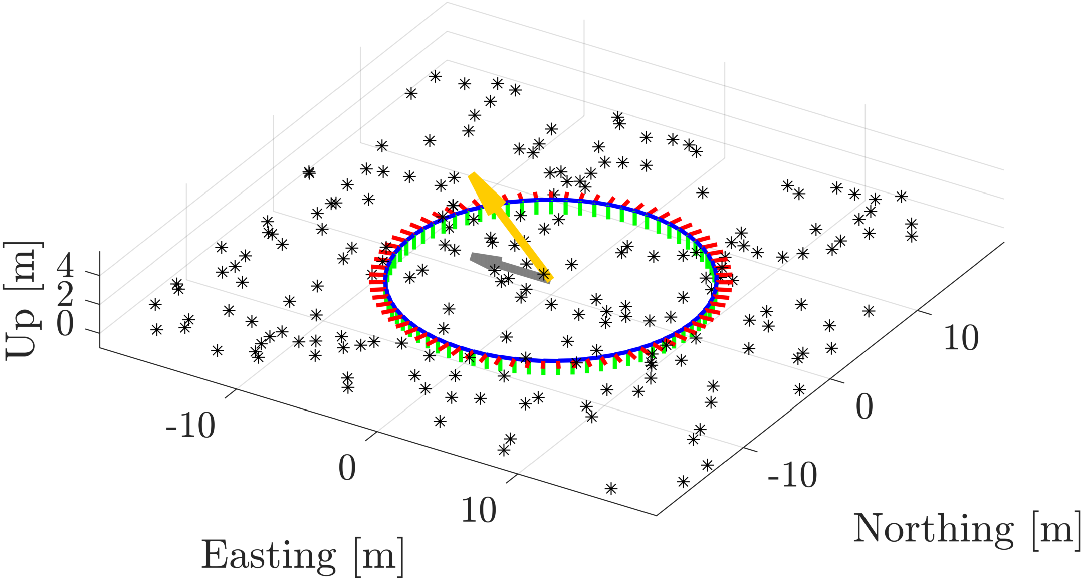
\includegraphics[width=\textwidth]{sims_circle200_environment}
%%     \caption{``Circle'' trajectory}
%% \end{subfigure}
%\begin{subfigure}{0.45\textwidth}
%    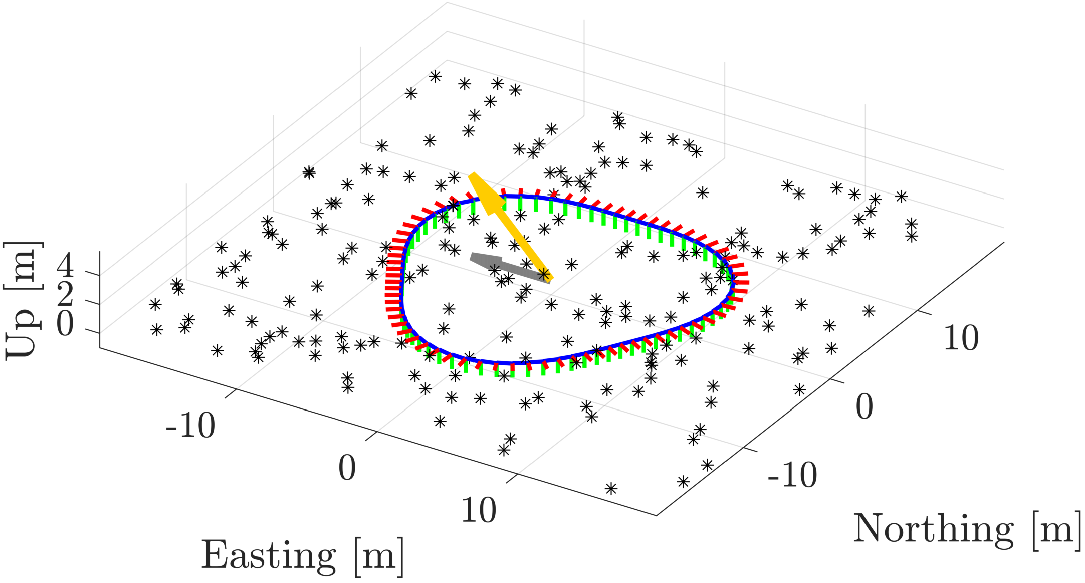
\includegraphics[width=\textwidth]{sun-bcnn/sims/sims_triangle200_environment}
%    \caption{``Triangle'' trajectory}
%\end{subfigure}
%~
%\begin{subfigure}{0.45\textwidth}
%    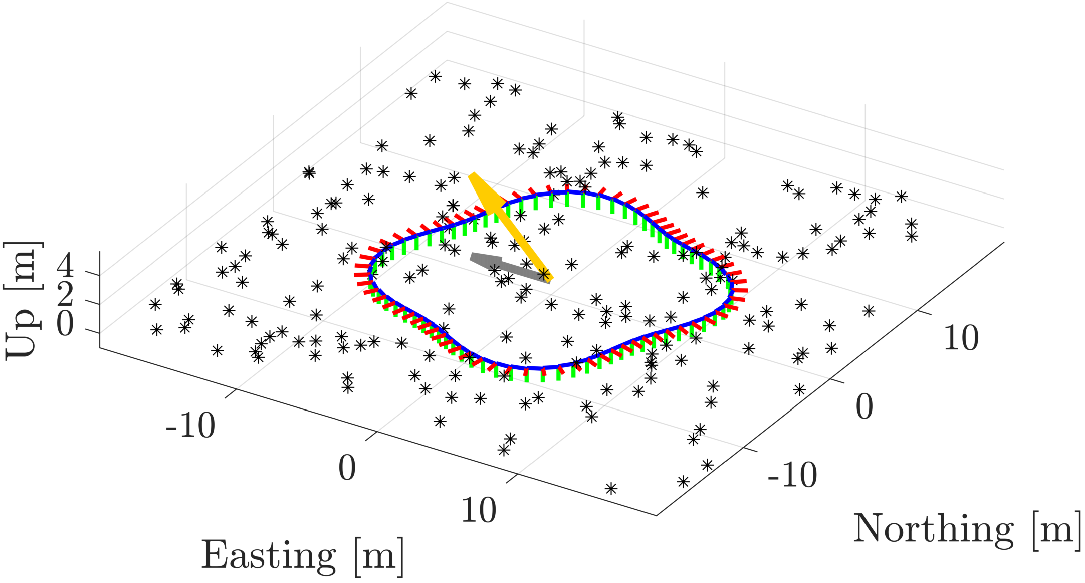
\includegraphics[width=\textwidth]{sun-bcnn/sims/sims_square200_environment}
%    \caption{``Square'' trajectory}
%\end{subfigure}
%~
%\begin{subfigure}{0.45\textwidth}
%    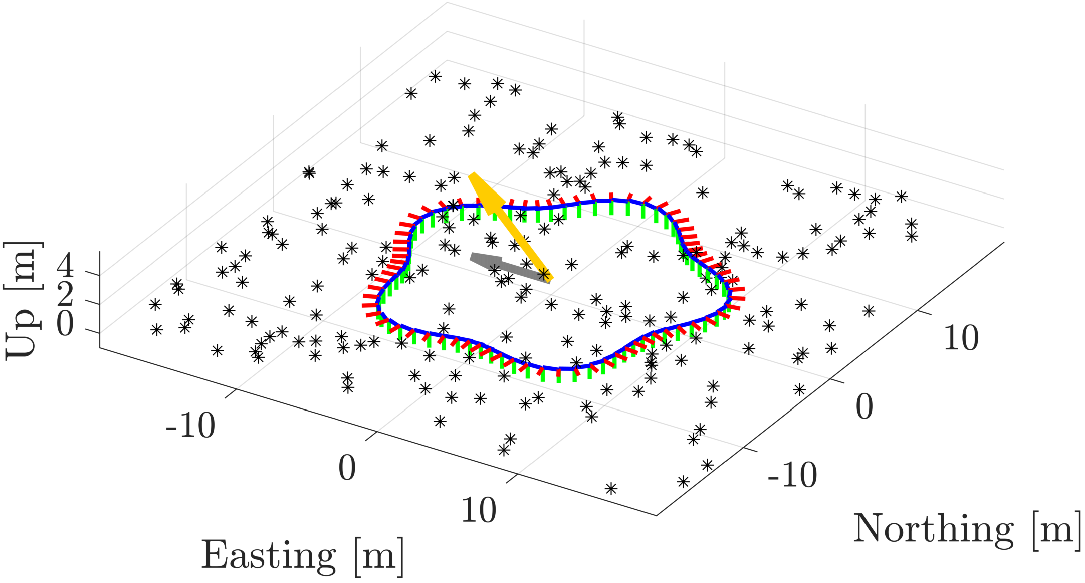
\includegraphics[width=\textwidth]{sun-bcnn/sims/sims_penta200_environment}
%    \caption{``Star'' trajectory}
%\end{subfigure}
%\caption{One loop of the ``Triangle'', ``Square'', and ``Star'' trajectories, consisting primarily of translation and yaw rotation. Landmarks are shown as black asterisks, and the simulated sun direction is indicated with a yellow arrow along with its projection, in grey, on the EN-plane.}
%\label{fig:sim_environment}
%\end{figure*}
%
%\begin{figure*}
%\centering
%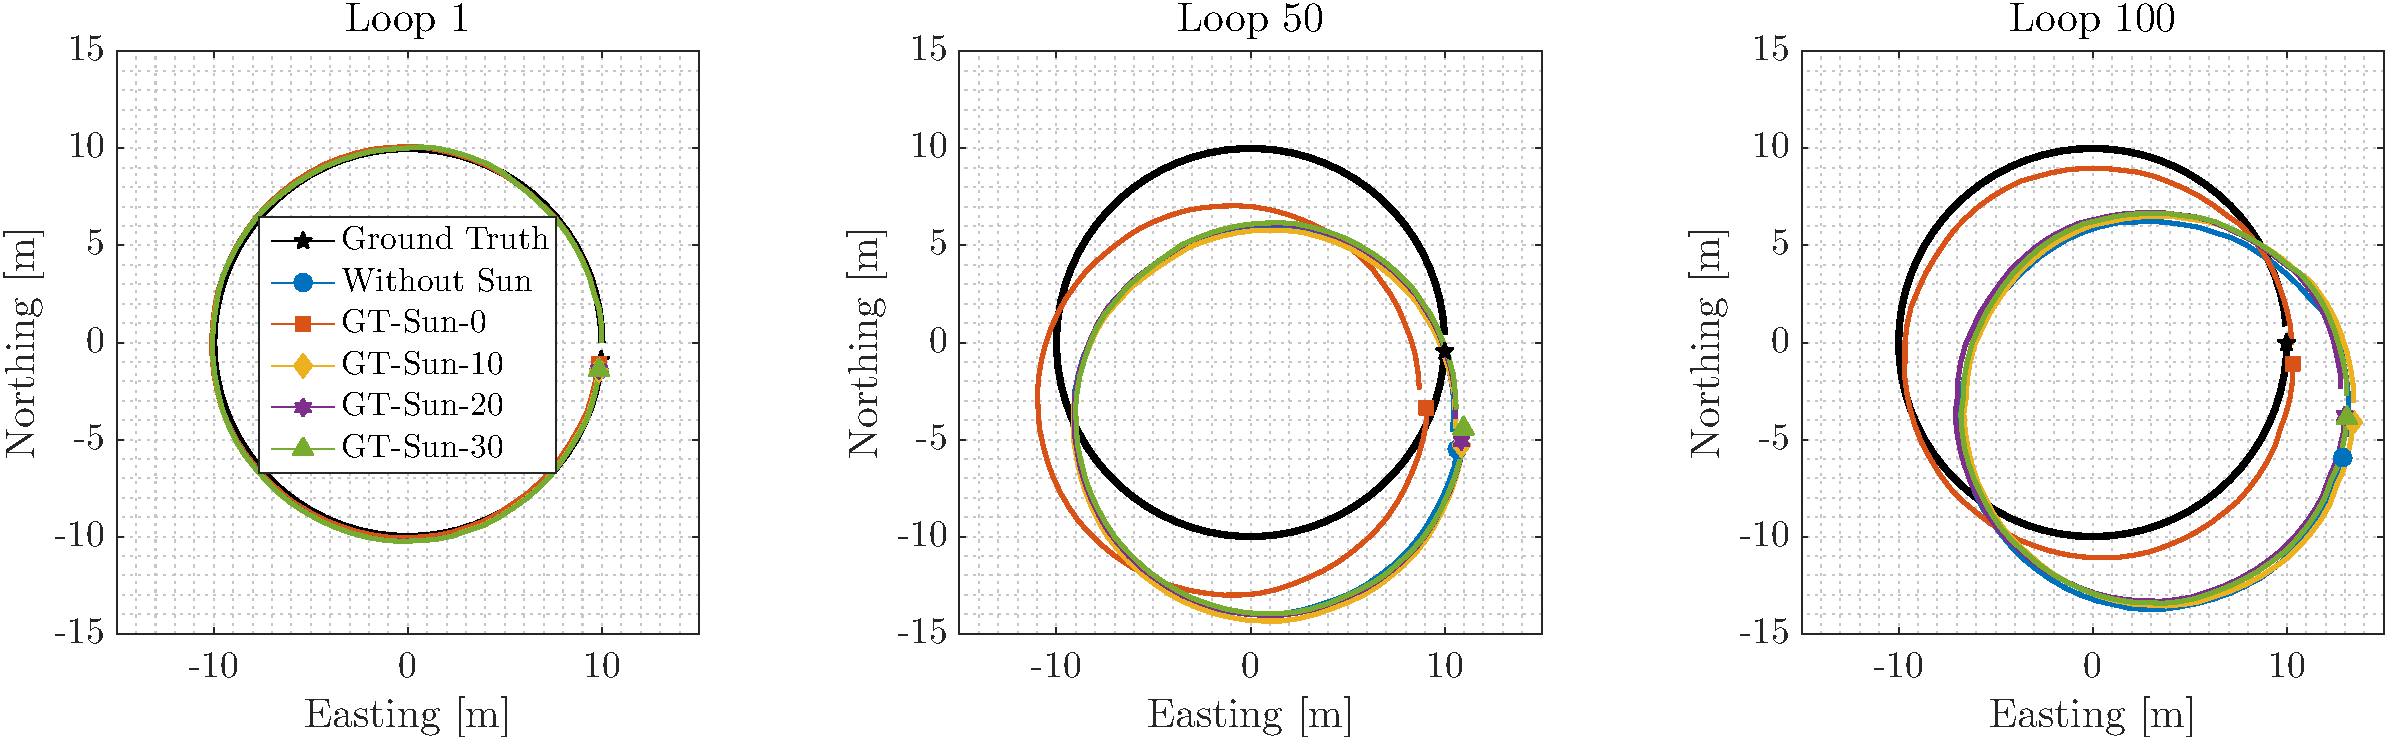
\includegraphics[width=0.98\textwidth]{sun-bcnn/sims/sims_circle200_traj}
%\caption{Selected segments of a 100-loop ``Circle'' trajectory, without sun corrections, and with sun corrections corrupted by varying levels of artificial Gaussian noise. The effect of VO drift can be clearly seen, as well as the benefit of incorporating observations of a directional landmark such as the sun.}
%\label{fig:sim_topdown}
%\end{figure*}
%
%\begin{figure*}
%\centering
%	 \begin{subfigure}{0.42\textwidth}
%	 	\vspace{-5pt}
%    	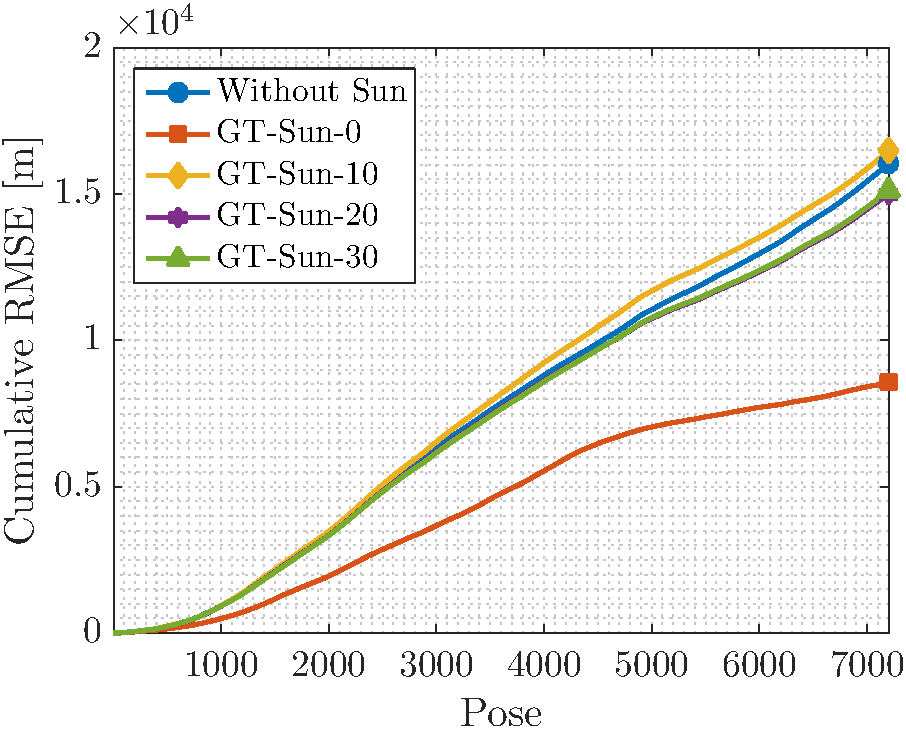
\includegraphics[width=\textwidth]{sun-bcnn/sims/sims_circle200_enu_rmse}
%        \caption{Translational CRMSE (ENU)}
%        \label{fig:sim_traj}
%    \end{subfigure}
%    ~
%    \begin{subfigure}{0.42\textwidth}
%    	\vspace{-5pt}
%    	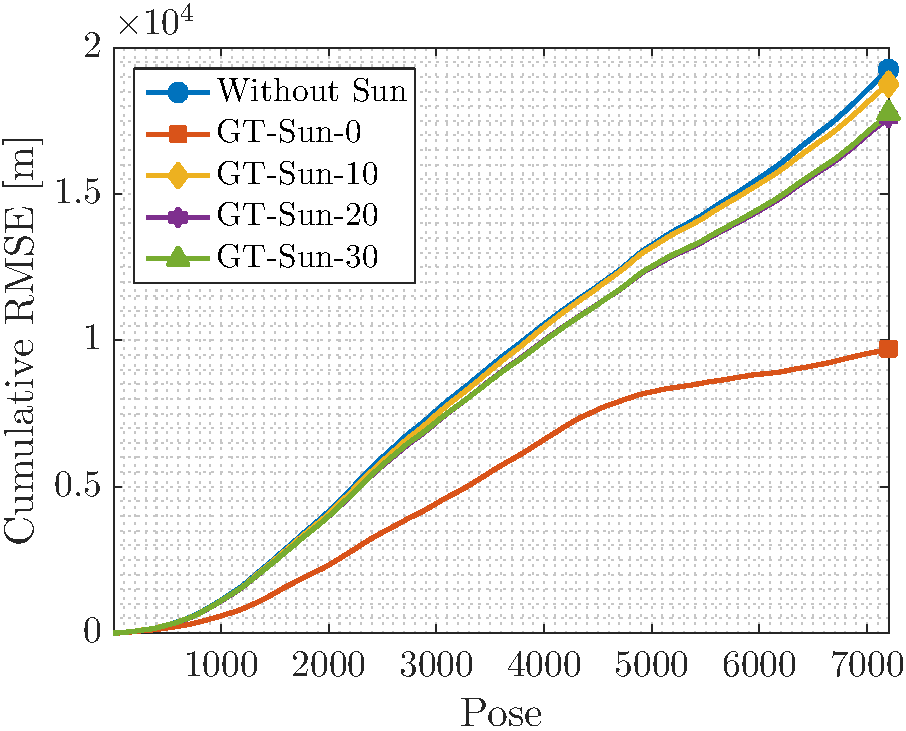
\includegraphics[width=\textwidth]{sun-bcnn/sims/sims_circle200_en_rmse}
%        \caption{Translational CRMSE (EN plane)}
%        \label{fig:sim_en_rmse}
%    \end{subfigure}
%    ~
%    \begin{subfigure}{0.42\textwidth}
%    	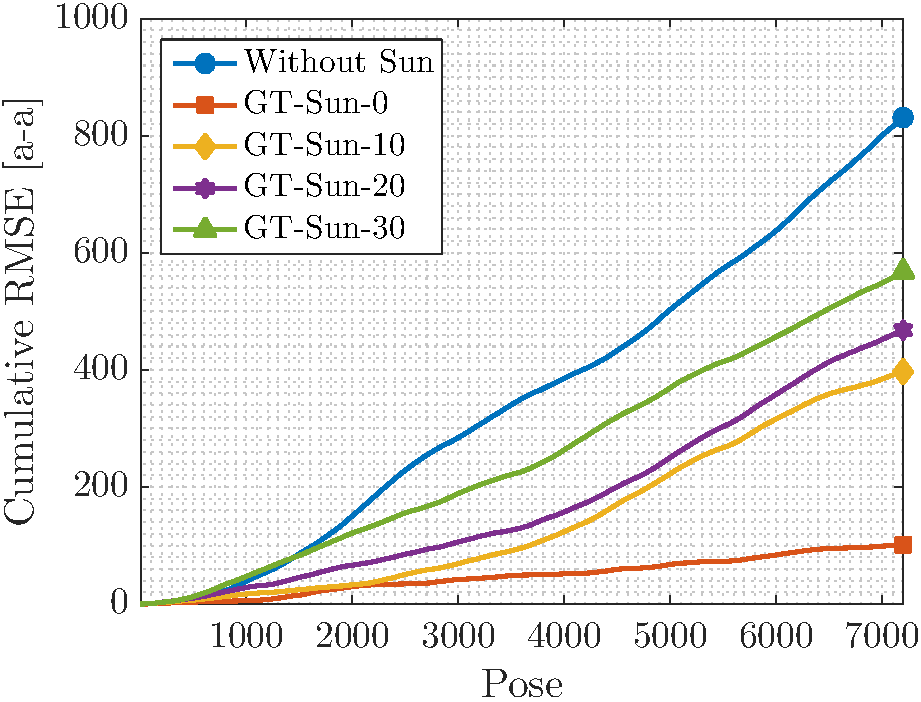
\includegraphics[width=\textwidth]{sun-bcnn/sims/sims_circle200_rot_rmse}
%        \caption{Rotational CRMSE}
%        \label{fig:sim_rot_rmse}
%    \end{subfigure}
%
%\caption{Cumulative root mean squared error (CRMSE) of a simulated 100-loop circular trajectory, without sun corrections, and with sun corrections corrupted by varying levels of artificial Gaussian noise. The accumulated estimation error is greatly reduced by incorporating observations of the sun, and the benefit decreases as these observations become noisier.}
%\label{fig:sim_rmse}
%\end{figure*}
%
%\begin{table}[]
%\centering
%\caption{Comparison of translational and rotational average root mean squared errors (ARMSE) on simulated sequences.}
%\label{tab:sim_armse}
%\begin{tabular}{@{}lcccc@{}}
%\textbf{Loop Shape}                                  & Circle & Triangle & Square & Star   \\ \midrule
%\textbf{\# Loops}                             & 100    & 100      & 100    & 100    \\ \midrule
%\multicolumn{5}{@{}l@{}}{\textbf{Trans. ARMSE {[}m{]}}  } \\
%\quad Without Sun & 2.22 & 2.00 & 2.33 & 1.41 \T\B \\
%\quad GT-Sun-0    & 1.19 & 1.62 & 2.13 & 0.75 \T \\
%\quad GT-Sun-10   & 2.29 & 2.07 & 2.05 & 1.32 \\
%\quad GT-Sun-20   & 2.08 & 2.12 & 2.31 & 1.33 \\
%\quad GT-Sun-30   & 2.10 & 1.95 & 2.16 & 1.38 \\ \midrule
%\multicolumn{5}{@{}l@{}}{\textbf{Trans. ARMSE (EN-plane) {[}m{]}}} \\
%\quad Without Sun & 2.67 & 1.88 & 2.57 & 1.10 \T\B \\
%\quad GT-Sun-0    & 1.34 & 1.89 & 2.56 & 0.83 \T \\
%\quad GT-Sun-10   & 2.61 & 2.04 & 2.26 & 0.99 \\
%\quad GT-Sun-20   & 2.44 & 2.03 & 2.57 & 0.88 \\
%\quad GT-Sun-30   & 2.46 & 2.00 & 2.35 & 1.25 \\ \midrule
%\multicolumn{5}{@{}l@{}}{\textbf{Rot. ARMSE $\mathbf{(\times 10^{-3})}$ {[}axis-angle{]}}} \\
%\quad Without Sun & 115.32 & 144.56 & 107.27 & 111.19 \T\B \\
%\quad GT-Sun-0    & 14.10  & 113.58 & 59.21  & 30.69  \T \\
%\quad GT-Sun-10   & 55.22  & 115.03 & 75.62  & 39.17  \\
%\quad GT-Sun-20   & 65.02  & 121.11 & 80.41  & 49.75  \\
%\quad GT-Sun-30   & 78.73  & 145.22 & 100.91 & 72.39  \\ \bottomrule
%\end{tabular}
%\end{table}
%
%
%We assess the benefit of incorporating sun observations of varying quality by conducting a series of simulation experiments consisting of a stereo camera moving along loopy trajectories of varying shapes through a simulated field of point landmarks, with a single static directional landmark representing the sun.
%\Cref{fig:sim_environment} shows several such loopy trajectories.
%
%We simulate the sun at $45^\circ$ of zenith and an arbitrary azimuth angle, and corrupt observations of the ground truth sun vector with artificial noise such that the mean angular distance (a non-negative quantity) between the observed and true sun direction is $0^\circ$, $10^\circ$, $20^\circ$, and $30^\circ$, labeling these conditions \emph{GT-Sun-0}, \emph{GT-Sun-10}, \emph{GT-Sun-20}, and \emph{GT-Sun-30}, respectively.
%In our experiments, we treated the measurement noise as an additive quantity sampled from a zero-mean isotropic 3D Gaussian distribution, and renormalized the resulting vectors to enforce the unit-norm constraint.
%
%
%We simulate the sun at $45^\circ$ of zenith and an arbitrary azimuth angle, and corrupt observations of the ground truth sun vector with artificial noise such that the mean angular distance (a non-negative quantity computed from the dot product) between the ground truth and noisy sun vectors is $0^\circ$, $10^\circ$, $20^\circ$, or $30^\circ$.
%We label these conditions \emph{GT-Sun-0}, \emph{GT-Sun-10}, \emph{GT-Sun-20}, and \emph{GT-Sun-30}, respectively.
%We generated these noisy measurements by first sampling \mbox{3-vectors} from an isotropic zero-mean multivariate Gaussian distribution, then adding these vectors to the ground truth sun vector, and finally normalizing the result to unit length. 
%We chose the covariance of this distribution to yield the desired average angular distance in each case.
%Note that although the distribution from which we sample noise vectors is zero-mean, the average angular distances will not be zero-mean because angular distance is non-negative.
%
%
%Our choice to add noise in $\Real^3$ and re-normalize was motivated by the fact that this process yields approximately Gaussian error distributions over the azimuth and zenith error angles, which is an important property assumed by our VO pipeline to produce maximum likelihood motion estimates based on the fusion of multiple data sources.
%We note that these distributions are less Gaussian-like for larger covariances (due to the geometry of the unit 2-sphere) and for ground truth vectors near singularities (e.g., zero zenith).
%
%We also experimented with sampling simulated measurements from a Von Mises-Fisher distribution \citep{fisher1953dispersion}, which is approximately analogous to an isotropic Gaussian distribution that respects the geodesics on the unit 2-sphere.
%However, we observed that the resulting distributions on azimuth and zenith error were severely non-Gaussian, which violated the assumption of zero-mean Gaussian noise in our VO pipeline and interfered with our VO experiments.
%
%Since our VO pipeline does not incorporate loop closures, the effects of drift in the VO solution can be clearly seen by examining individual loops in the camera trajectory. 
%\Cref{fig:sim_topdown} shows three loops from the ``Circle'' trajectory, demonstrating that the VO solution drifts significantly from the true trajectory by the 100th loop.
%\Cref{fig:sim_rmse} plots the translational and rotational cumulative root mean squared error (CRMSE) for this trajectory, which measures the growth in total estimation error over time.
%\Cref{fig:sim_rot_rmse} in particular highlights the significant effect of sun sensing on rotational error, where we see a clear progression in estimation error as the sun direction observations become more noisy.
%
%\Cref{tab:sim_armse} shows that while all four simulation trajectories display consistent and predictable reductions in rotational average root mean squared error (ARMSE), this is not always the case for translational ARMSE.
%This is because translational errors are only partially induced by rotational errors, with the remainder made up of `sliding' motions orthogonal to the direction of travel.
%These non-rotational errors are highly dependent on the specific trajectory, where more or less of the observed feature tracks can be explained by a sliding motion instead of a rotation.
%Due to the coupling of translational and rotational errors, correcting for rotational error in such cases may actually worsen the translational error (e.g., on the ``Triangle'' sequence).
%
%While we do not implement this in our work, we speculate that incorporating an appropriate motion model into our VO formulation would significantly mitigate the impact of these errors by, for example, imposing a nonholonomic constraint on a ground vehicle or accounting for the dynamics of a quadcopter.

%%%%%%%%%%%%%%%%%%%%%%%%%%%%%%%%%%%%%%%%
% EXPERIMENTS: KITTI
%%%%%%%%%%%%%%%%%%%%%%%%%%%%%%%%%%%%%%%%
\section{Urban Driving Experiments: The KITTI Odometry Benchmark}
\begin{figure}
    \centering
    \begin{subfigure}[b]{0.75\textwidth}
        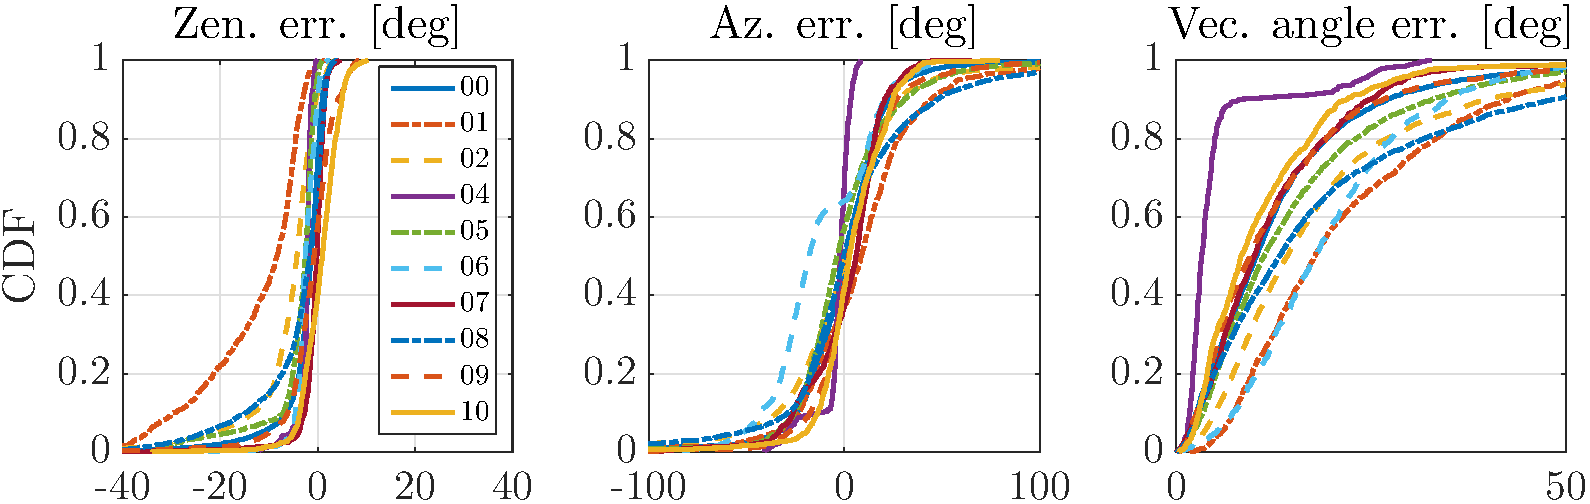
\includegraphics[width=\textwidth]{sun-bcnn/kitti/kitti_cdf}
    \end{subfigure} ~
    \begin{subfigure}[b]{0.75\textwidth}
        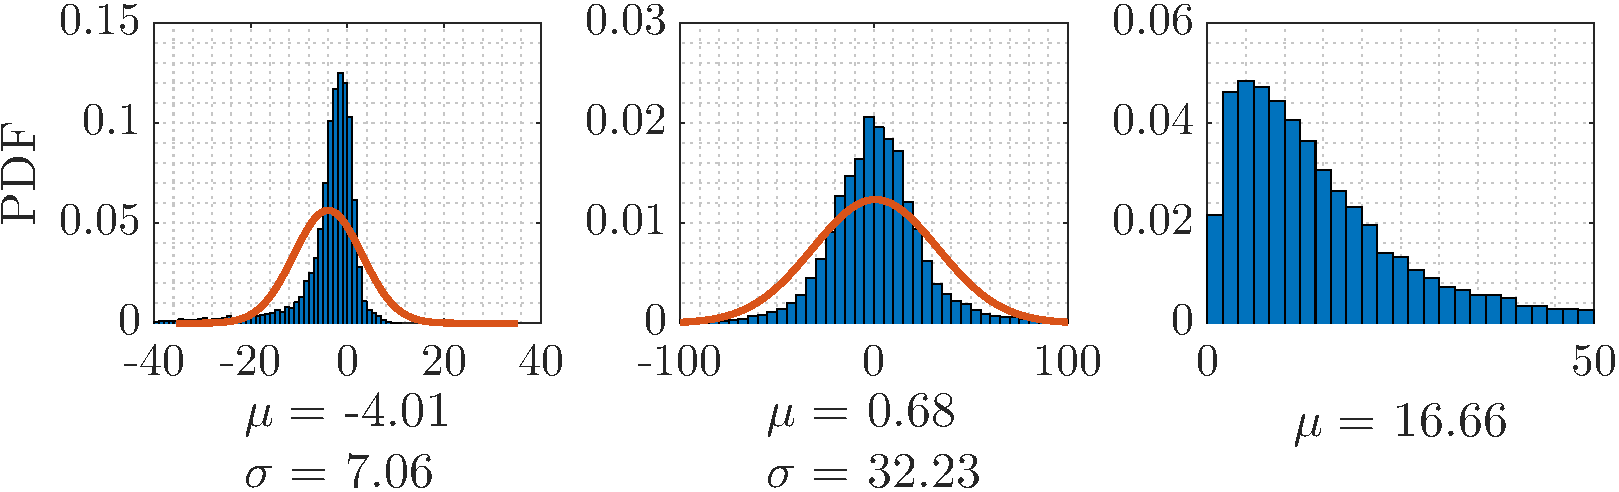
\includegraphics[width=\textwidth]{sun-bcnn/kitti/kitti_hist_azzen}
    \end{subfigure}
    \caption{Distributions of azimuth error, zenith error, and angular distance for Sun-BCNN compared to ground truth over each test sequence in the KITTI dataset. \emph{Top row}: Cumulative distributions of errors for each test sequence individually. \emph{Bottom row:} Histograms and Gaussian fits of aggregated errors.}
    \label{fig:sun-bcnn_kitti_cnn_testerrors}
\end{figure}

\begin{figure}
    \centering
    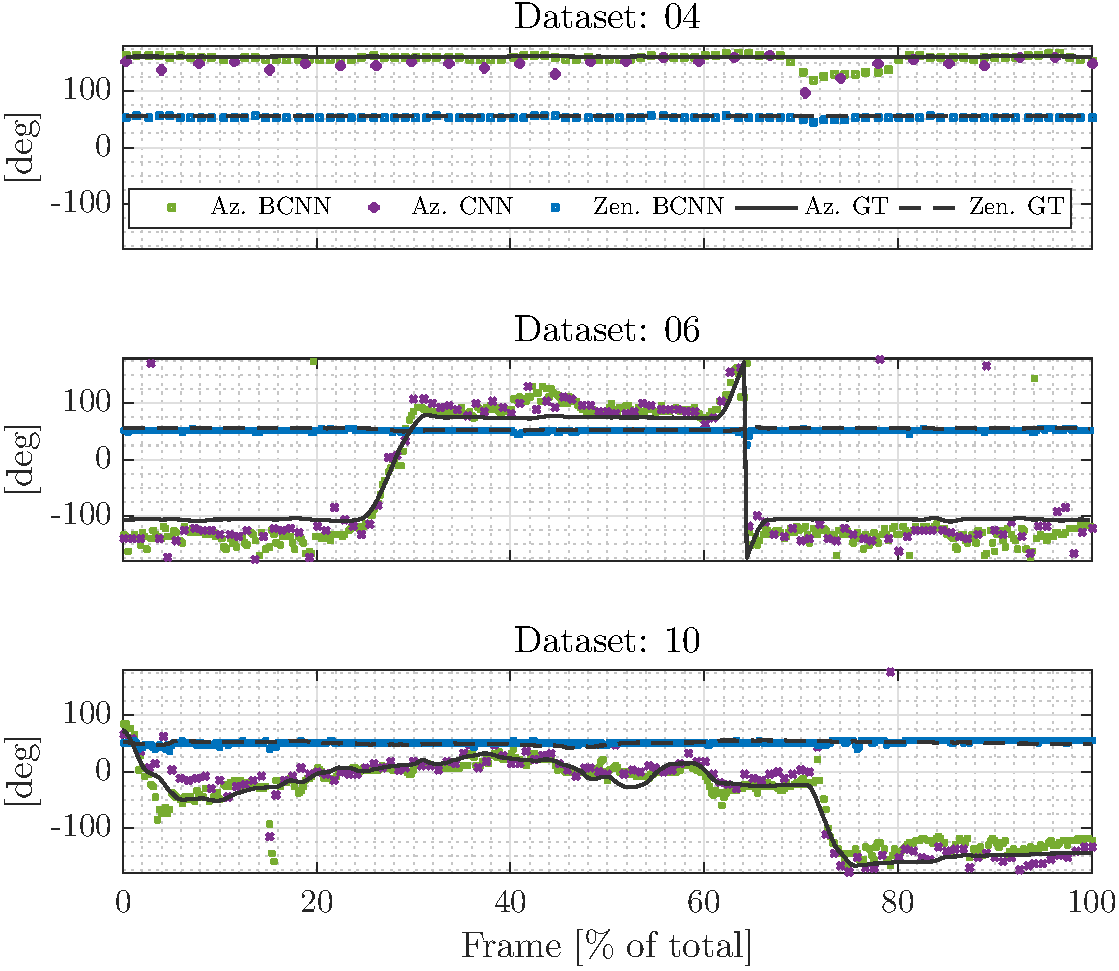
\includegraphics[width=0.75\textwidth]{sun-bcnn/kitti/kitti_error_over_time}
    \caption{Azimuth (Sun-CNN and Sun-BCNN) and zenith (Sun-BCNN only) predictions over time for KITTI test sequences \texttt{04}, \texttt{06} and \texttt{10}. Sun-CNN is trained and tested on every tenth image, whereas Sun-BCNN is trained and tested on every image. In our VO experiments, we use the Sun-BCNN predictions of every tenth image to make a fair comparison. }
    %\vspace{-0.4em}
    \label{fig:sun-bcnn_kitti_error_over_time}
\end{figure}

\begin{table}
\centering
\caption{Test Errors for Sun-BCNN on KITTI odometry sequences with estimates computed at every image.}
\resizebox{\columnwidth}{!}{%
\label{tab:kitti_test_cnn}
\begin{threeparttable}
\begin{tabular}{@{}cccccccccccccccc@{}}
         &  & \multicolumn{3}{c}{\textbf{Zenith Error {[}deg{]}}} &  & \multicolumn{3}{c}{\textbf{Azimuth Error {[}deg{]}}} &  & \multicolumn{3}{c}{\textbf{Vector Angle Error {[}deg{]}}} & & \B \\ \cline{3-5} \cline{7-9} \cline{11-13} 
\textbf{Sequence} &  & Mean          & Median       & Stdev       &  & Mean         & Median        & Stdev        &  & Mean           & Median          & Stdev & & \textbf{ANEES}\tnote{1}         \T \\ \midrule
\texttt{00}     &  & -2.59  & -1.37  & 5.15           &  & -0.33  & 0.81   & 25.61           &  & 13.56 & 10.31  & 13.14 &  & 1.00 \T \\
\texttt{01}     &  & -12.53 & -8.31  & 10.33          &  & 8.95   & 8.83   & 33.67           &  & 22.16 & 17.85  & 15.00 &  & 1.38 \\
\texttt{02}     &  & -6.13  & -4.26  & 7.38           &  & -1.03  & 0.74   & 37.61           &  & 19.69 & 14.32  & 18.25 &  & 1.40 \\
\texttt{04}     &  & -2.42  & -2.11  & 1.64           &  & -3.89  & -2.18  & 9.14            &  & 5.33  & 3.29   & 6.44  &  & 0.30 \\
\texttt{05}     &  & -4.31  & -2.51  & 6.18           &  & -0.74  & -3.80  & 29.81           &  & 15.66 & 11.33  & 14.80 &  & 1.05 \\
\texttt{06}     &  & -2.48  & -2.52  & 2.27           &  & -12.22 & -17.86 & 25.78           &  & 19.78 & 17.72  & 11.35 &  & 1.93 \\
\texttt{07}     &  & -0.69  & -0.16  & 3.26           &  & 1.25   & 5.98   & 20.27           &  & 12.44 & 10.05  & 9.97  &  & 0.97 \\
\texttt{08}     &  & -4.46  & -1.61  & 8.14           &  & 3.66   & -0.14  & 41.73           &  & 19.90 & 13.30  & 19.59 &  & 1.04 \\
\texttt{09}     &  & -1.35  & -0.75  & 5.60           &  & 4.78   & 2.36   & 23.84           &  & 13.09 & 9.48   & 12.66 &  & 0.73 \\
\texttt{10}     &  & 0.59   & 0.95   & 3.90           &  & 3.64   & 2.61   & 19.15           &  & 11.23 & 8.34   & 9.83  &  & 1.08 \B \\ \midrule
All                &  & -4.01  & -2.26  & 7.06           &  & 0.68   & 0.53   & 32.23           &  & 16.66 & 12.08  & 15.91 & & - &  \\ \bottomrule    
\end{tabular}
\begin{tablenotes}
	\item[1] We compute Average Normalized Estimation Error Squared (ANEES) values with all sun directions that fall below a cosine distance threshold of $0.3$ (relative to ground truth) and set $\tau^{-1} = 0.015$.
 \end{tablenotes}
\end{threeparttable}
}
\end{table}

\begin{figure}
    \centering
    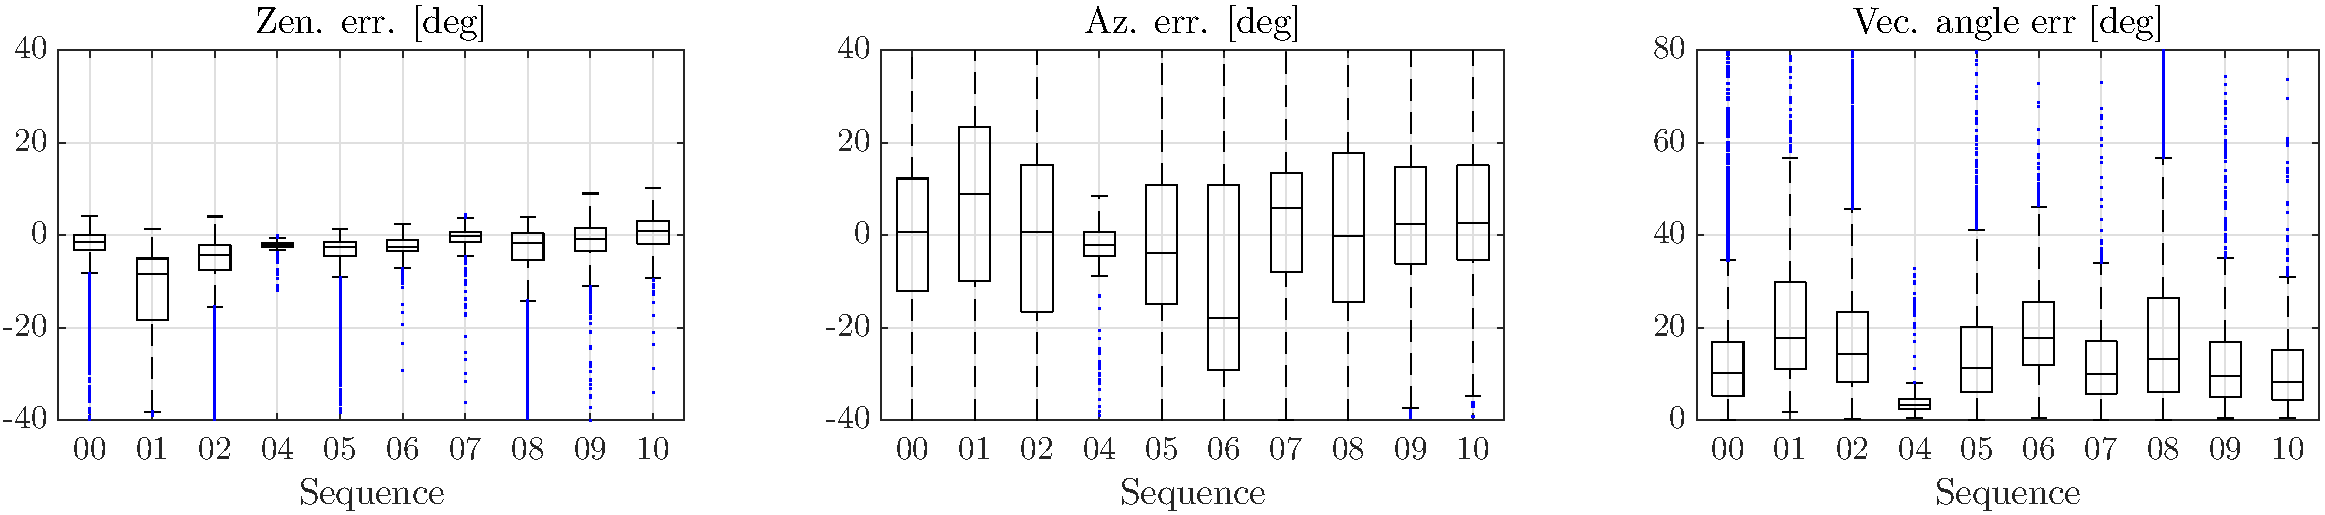
\includegraphics[width=0.98\textwidth]{sun-bcnn/kitti/kitti_testStatsBoxPlot}
    \caption{Box-and-whiskers plot of final test errors on all ten KITTI odometry sequences (c.f. \Cref{tab:kitti_test_cnn}).}
%    \vspace{-0.4em}
    \label{fig:kitti_test_error_whiskers}
\end{figure}

\begin{figure}
	\centering
	 \begin{subfigure}{0.42\textwidth}
    	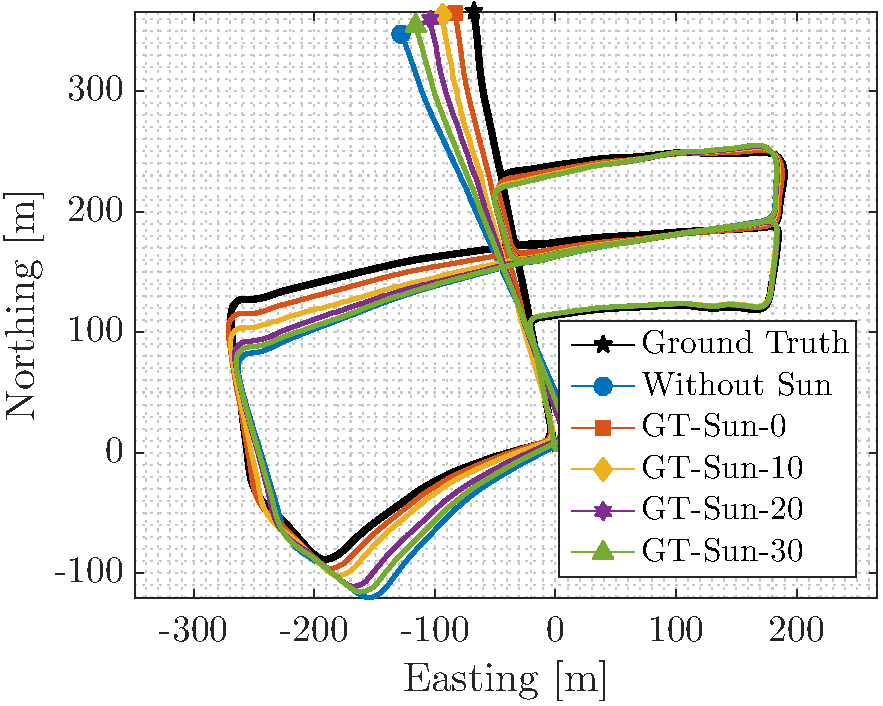
\includegraphics[width=\textwidth]{sun-bcnn/kitti/kitti_05_traj_sim}
        \caption{VO and ground truth trajectories}
    \end{subfigure}
    ~
    \begin{subfigure}{0.42\textwidth}
    	\vspace{-8pt}
    	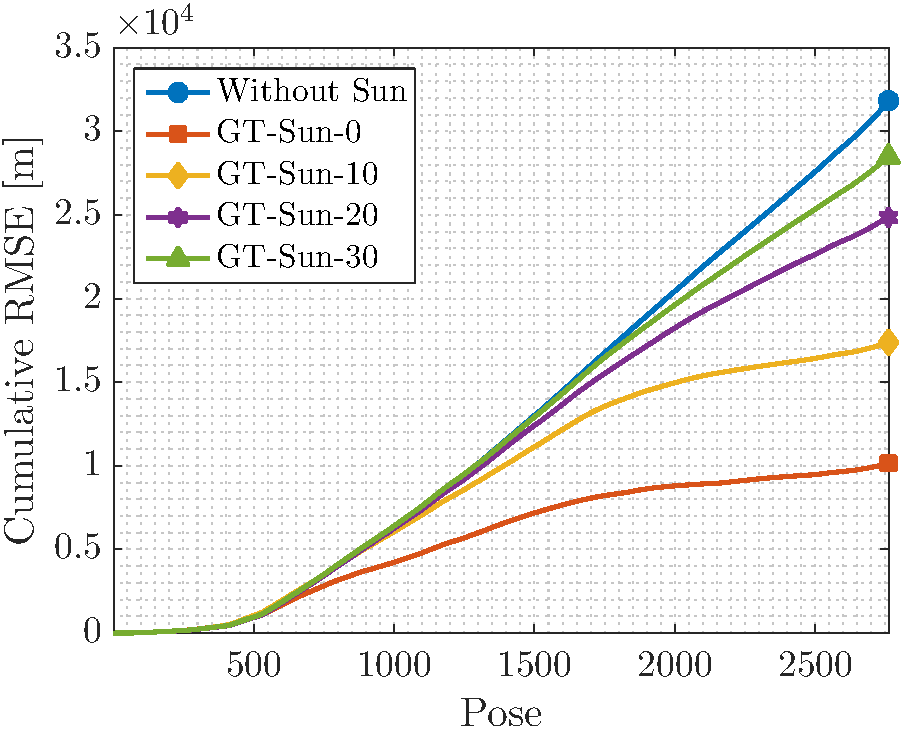
\includegraphics[width=\textwidth]{sun-bcnn/kitti/kitti_05_en_rmse_sim}
        \caption{Translational CRMSE (EN-plane)}
    \end{subfigure}
    ~
    \begin{subfigure}{0.42\textwidth}
    	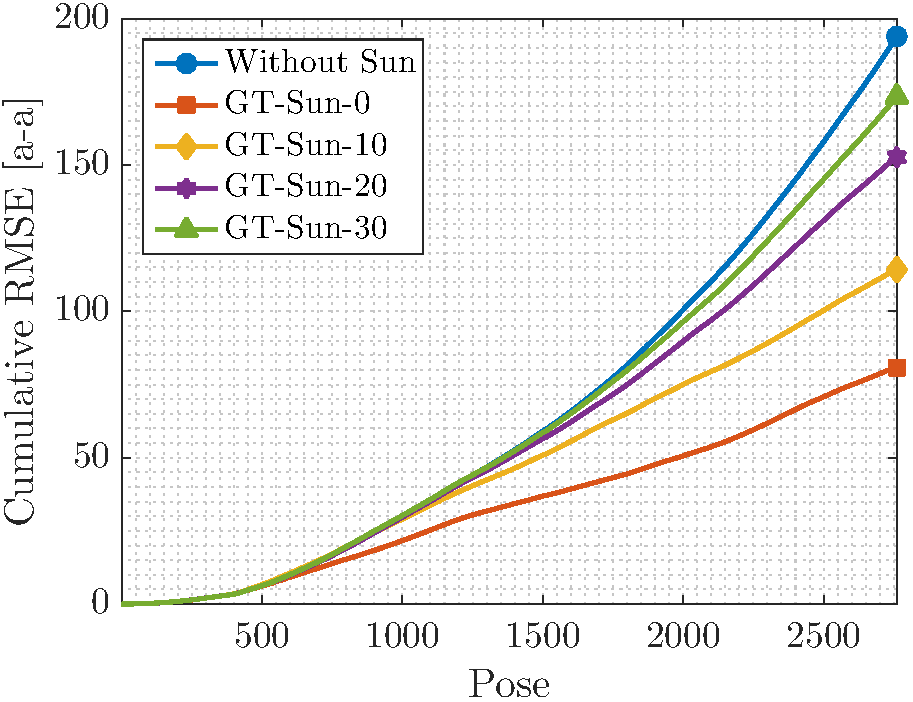
\includegraphics[width=\textwidth]{sun-bcnn/kitti/kitti_05_rot_rmse_sim}
        \caption{Rotational CRMSE}
    \end{subfigure}

    \caption{VO results for KITTI odometry sequence \texttt{05} using simulated sun measurements at every tenth pose. We observe a clear progression in cumulative root mean squared error (CRMSE) in translation and rotation as noise in the simulated sun measurements increases.}
     \label{fig:kitti-vo-sim-results}
\end{figure}

We investigated the performance of Sun-BCNN on the KITTI odometry benchmark training set \citep{Geiger2013-ky}, which consists of 21.6 km of urban driving data\footnote{Because we rely on the first pose reported by the GPS/INS system, we used the raw (rectified and synchronized) sequences corresponding to each odometry sequence. However, the raw sequence \texttt{2011\_09\_26\_drive\_0067} corresponding to odometry sequence \texttt{03} was not available on the KITTI website at the time of writing, so we omit sequence \texttt{03} from our analysis.}.
Importantly, the dataset includes 6-DOF ground truth poses obtained from an accurate GPS/INS tracking system, as well as calibrated transformations between this sensor and the colour stereo pair we use for sun estimation and VO in our experiments.
This allows us to create a training set of ground truth sun vectors for each image by querying the solar ephemeris model at each ground truth pose and rotating the resulting vector from the GPS/INS frame $\CoordinateFrame{0}$ (which is an ENU coordinate system) into the camera coordinate frame $\CoordinateFrame{k}$.
For each of our experiments, we trained Sun-BCNN on nine benchmark sequences and tested on the remaining sequence.
This procedure is consistent with that of \citet{Ma2016-at}, against whose Sun-CNN we directly compare, and allows us to evaluate each sequence using the maximum amount of training data.

\begin{figure*}[h]
	\centering
	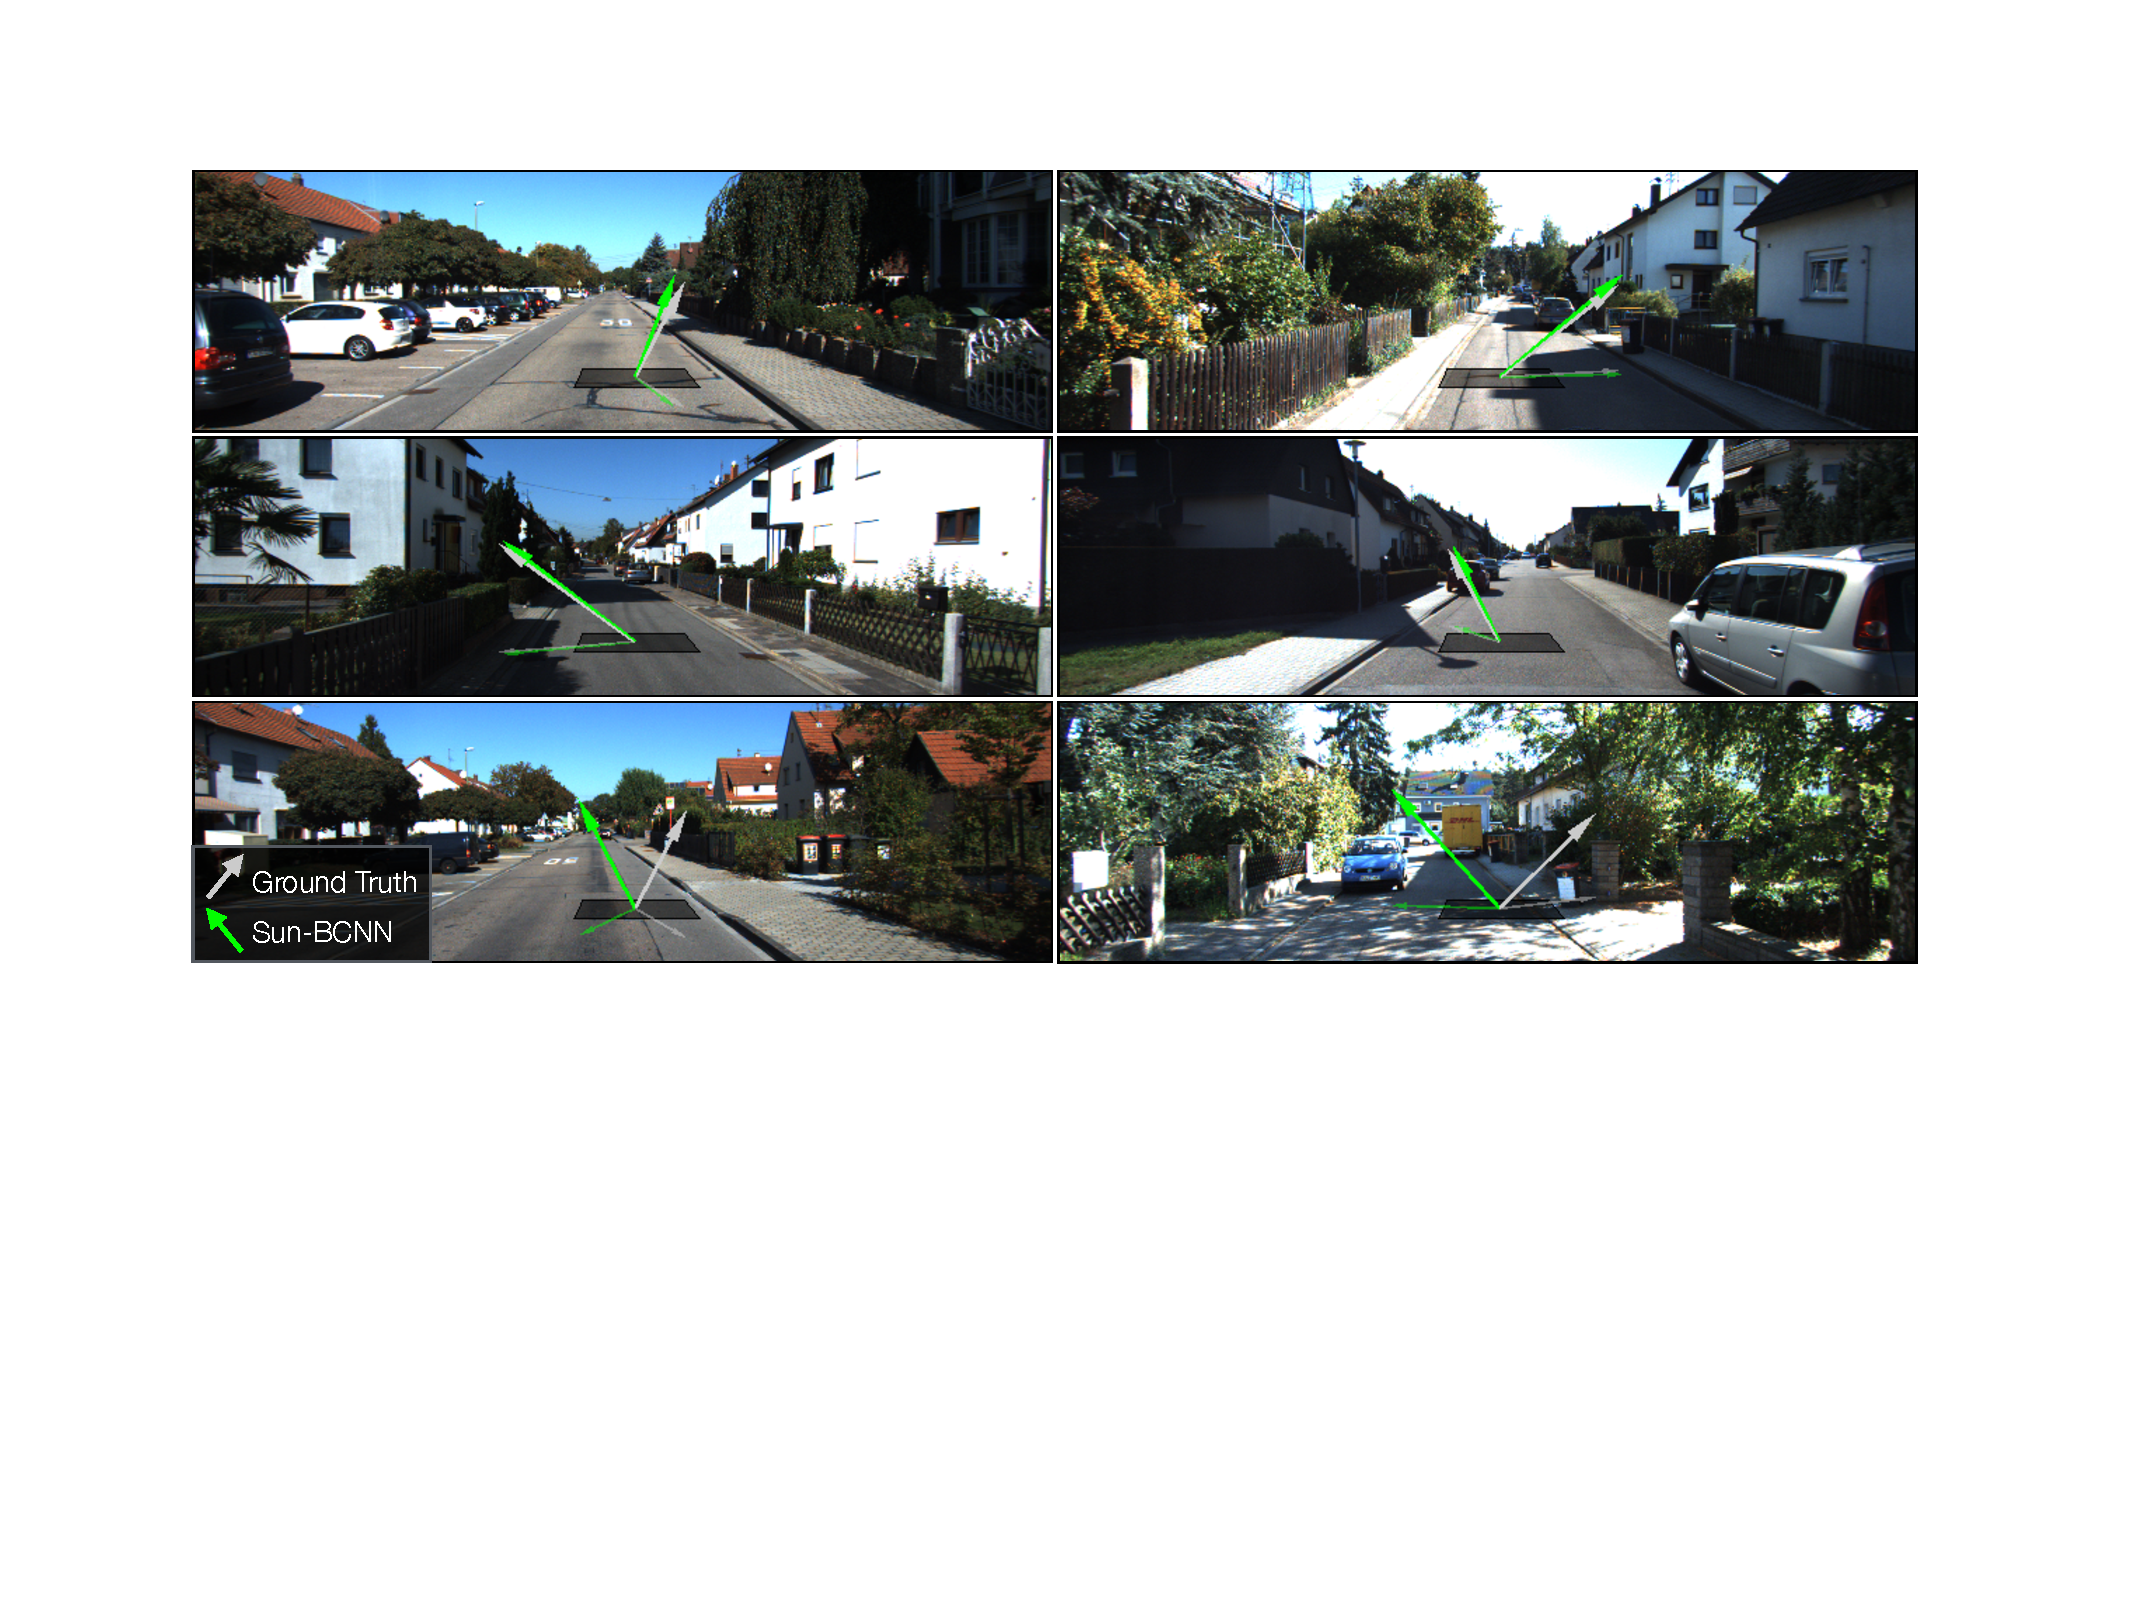
\includegraphics[width=0.82\textwidth]{sun-bcnn/kitti/kitti_kitti_arrow_fig}	
	\caption{Sun BCNN predictions and associated ground truth sun directions on the KITTI sequence \texttt{05}. \emph{Top two rows}: Sun BCNN produces accurate predictions in a variety of azimuth values. \emph{Bottom row}: Poor results occur rarely due to shadow ambiguities.}
	\label{fig:kitti_arrows}
\end{figure*}

\begin{figure*}
	\centering
	 \begin{subfigure}{0.3\textwidth}
    	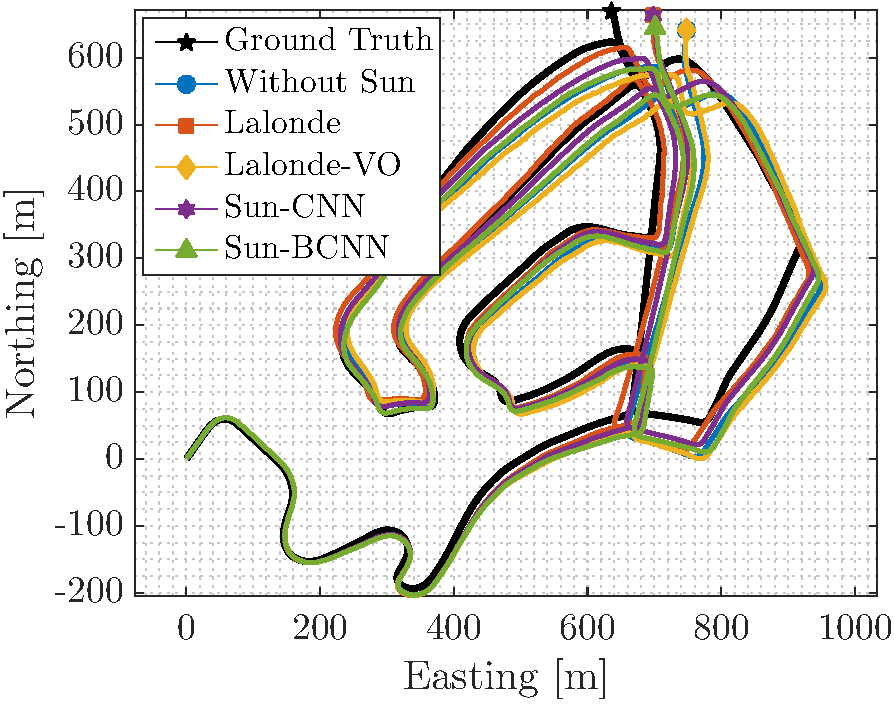
\includegraphics[width=\textwidth]{sun-bcnn/kitti/kitti_02_traj}
        \caption{\texttt{02}: VO and ground truth trajectories}
    \end{subfigure}
    ~
    \begin{subfigure}{0.3\textwidth}
    	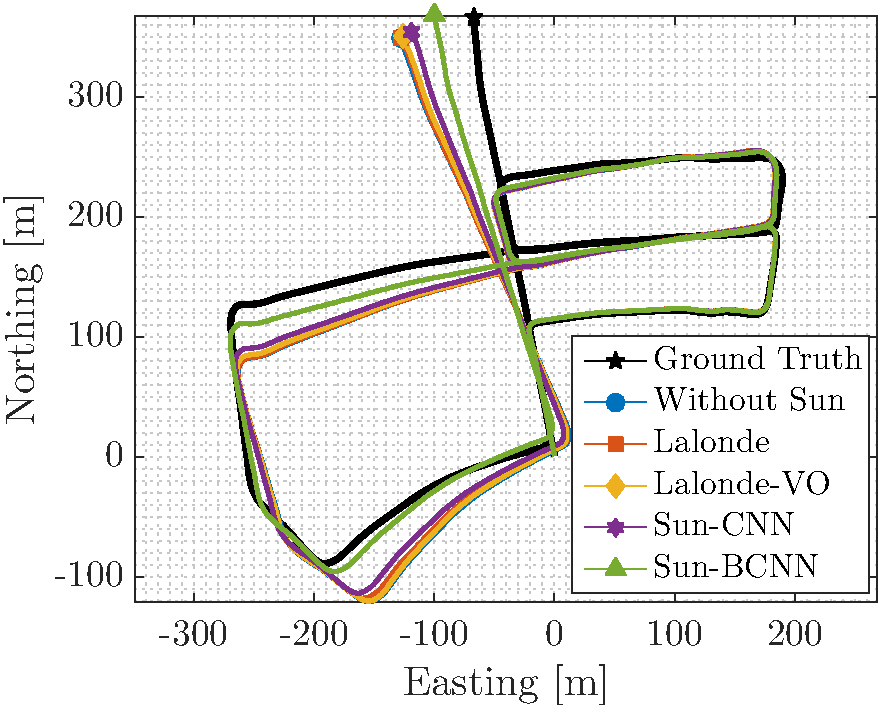
\includegraphics[width=\textwidth]{sun-bcnn/kitti/kitti_05_traj}
        \caption{\texttt{05}: VO and ground truth trajectories}
    \end{subfigure}
    ~
    \begin{subfigure}{0.3\textwidth}
    	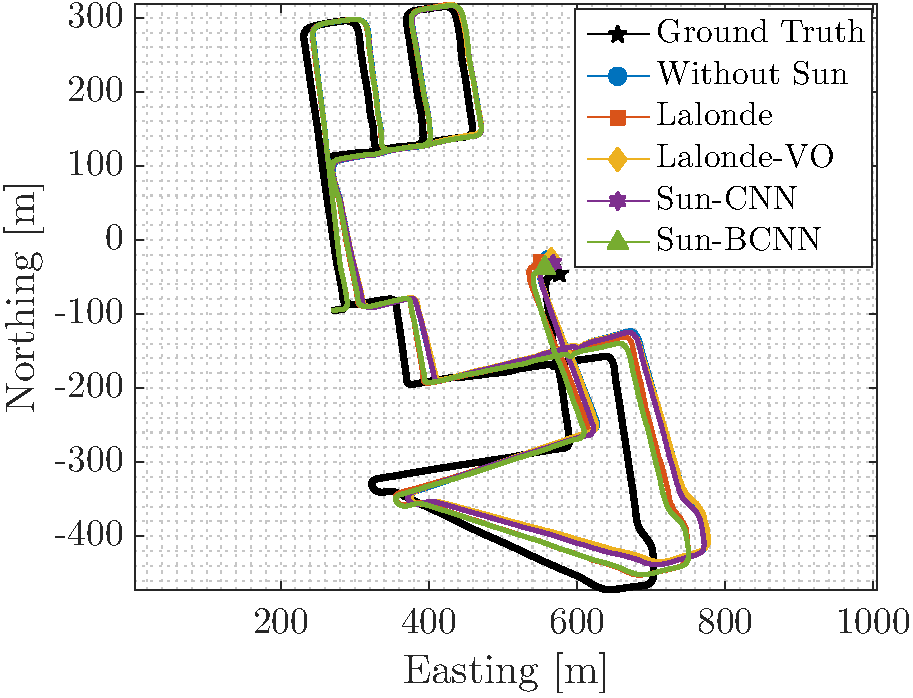
\includegraphics[width=\textwidth]{sun-bcnn/kitti/kitti_08_traj}
        \caption{\texttt{08}: VO and ground truth trajectories}
    \end{subfigure}
    \\
    \begin{subfigure}{0.3\textwidth}
    	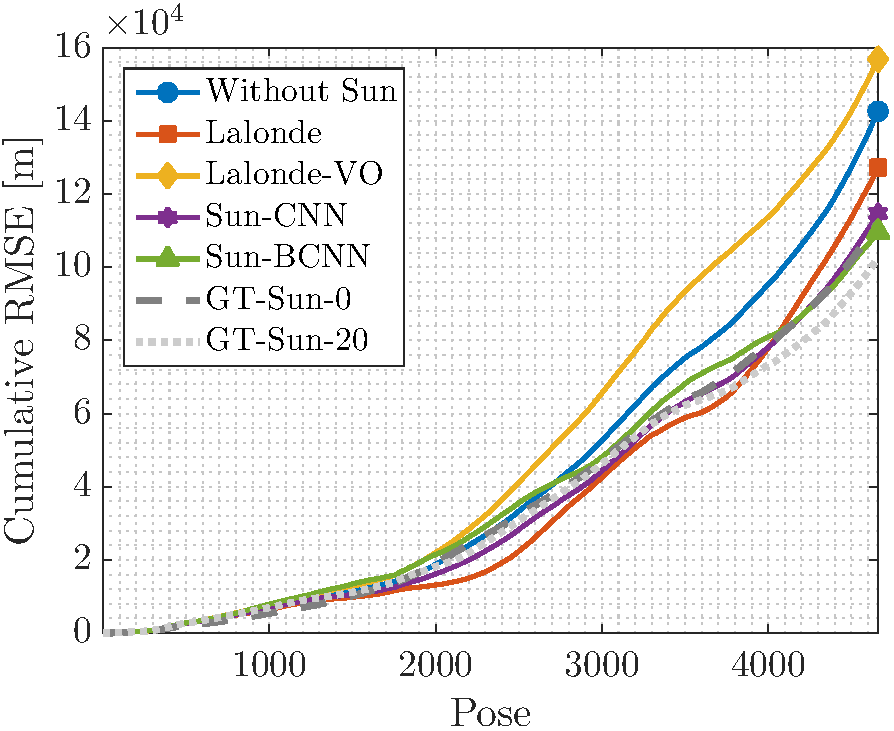
\includegraphics[width=\textwidth]{sun-bcnn/kitti/kitti_02_en_rmse}
        \caption{\texttt{02}: Translational CRMSE (EN-plane)}
    \end{subfigure}
    ~
    \begin{subfigure}{0.3\textwidth}
    	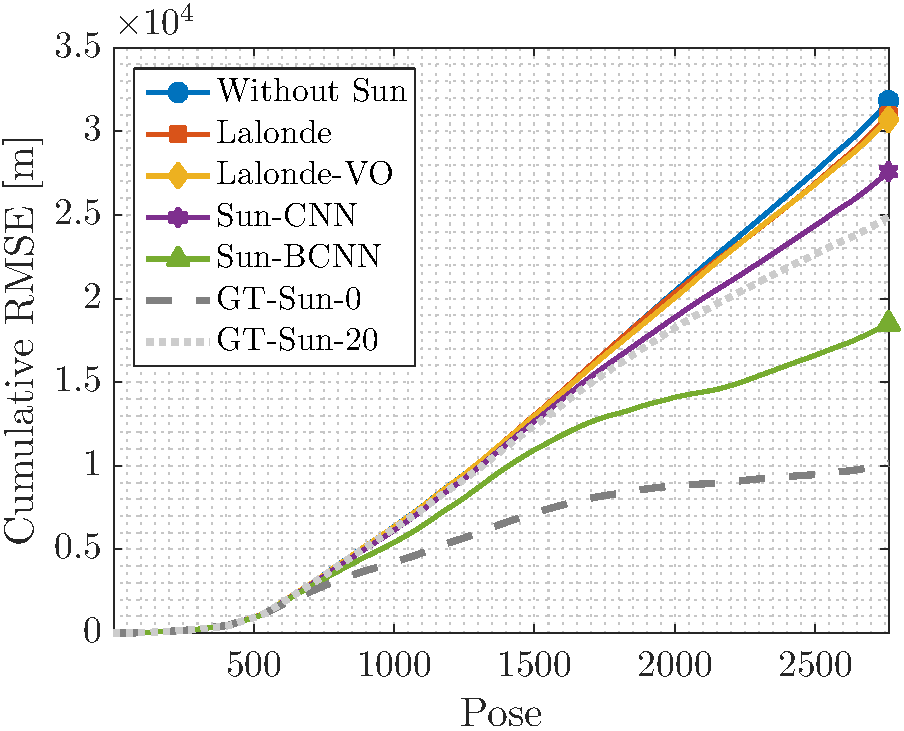
\includegraphics[width=\textwidth]{sun-bcnn/kitti/kitti_05_en_rmse}
        \caption{\texttt{05}: Translational CRMSE (EN-plane)}
    \end{subfigure}
    ~
    \begin{subfigure}{0.3\textwidth}
    	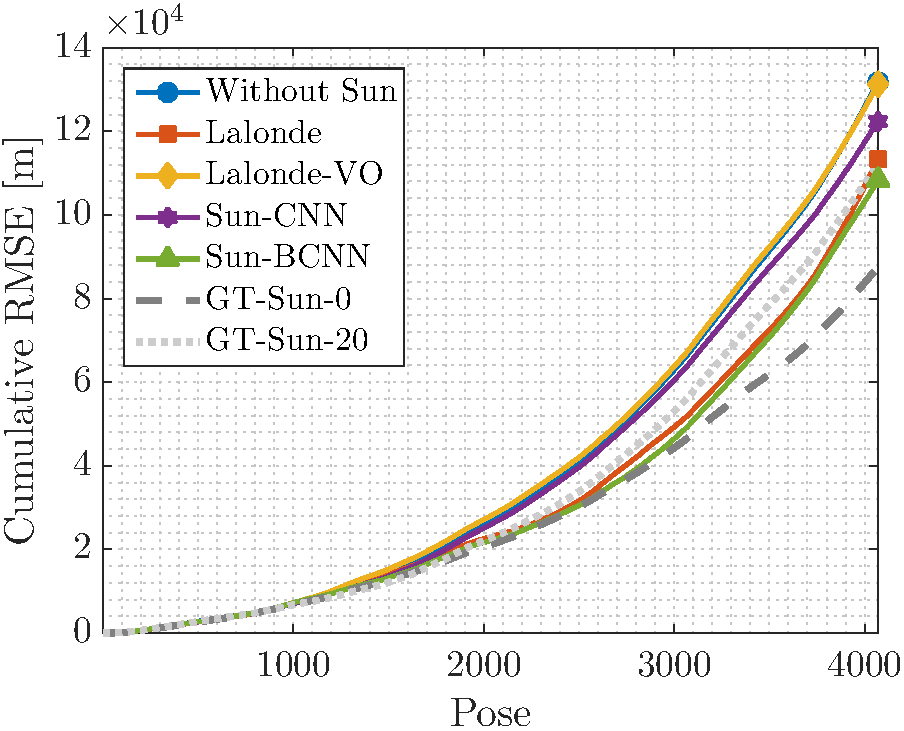
\includegraphics[width=\textwidth]{sun-bcnn/kitti/kitti_08_en_rmse}
        \caption{\texttt{08}: Translational CRMSE (EN-plane)}
    \end{subfigure}
    \\
    \begin{subfigure}{0.3\textwidth}
    	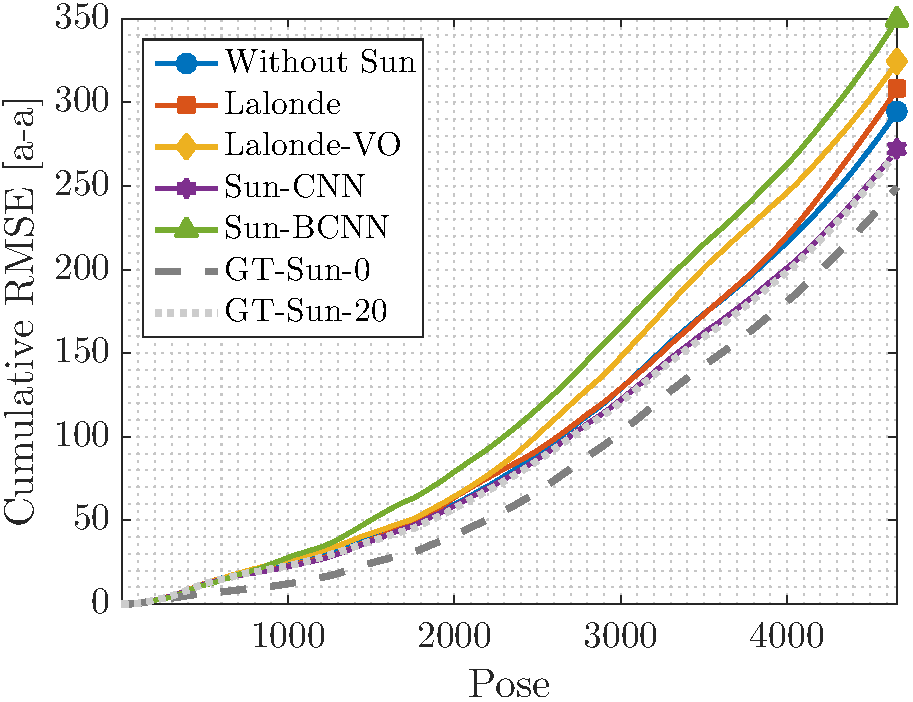
\includegraphics[width=\textwidth]{sun-bcnn/kitti/kitti_02_rot_rmse}
        \caption{\texttt{02}: Rotational CRMSE}
    \end{subfigure}
    ~
    \begin{subfigure}{0.3\textwidth}
    	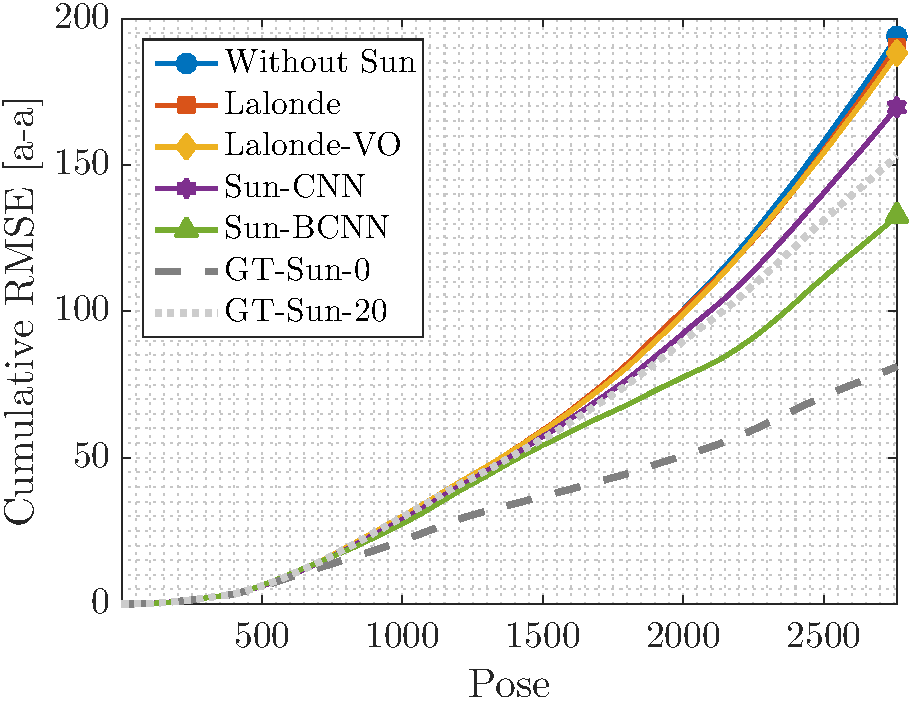
\includegraphics[width=\textwidth]{sun-bcnn/kitti/kitti_05_rot_rmse}
        \caption{\texttt{05}: Rotational CRMSE}
    \end{subfigure}
    ~
    \begin{subfigure}{0.3\textwidth}
    	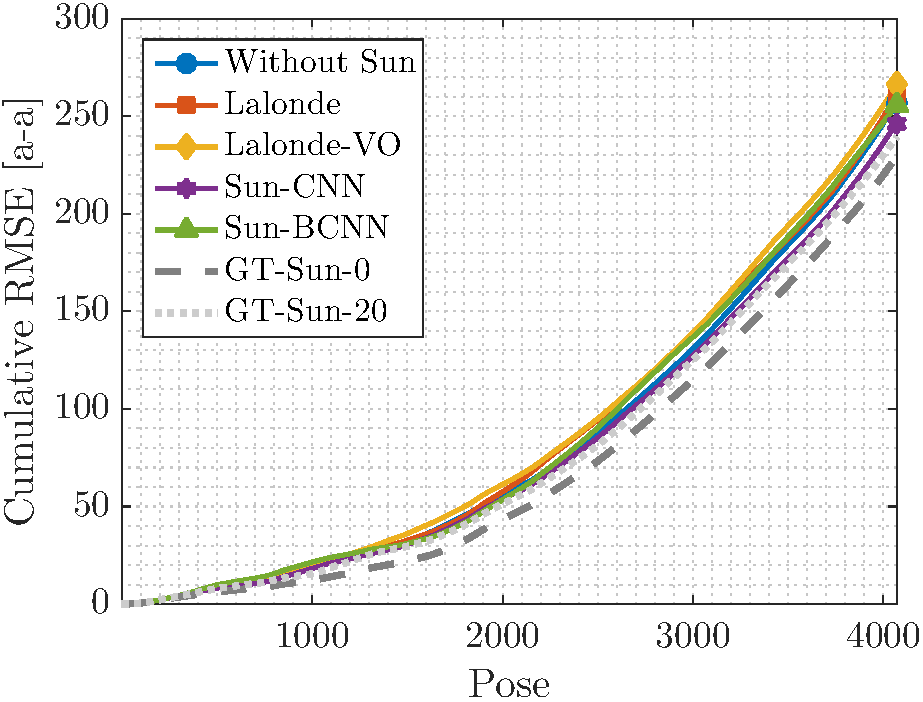
\includegraphics[width=\textwidth]{sun-bcnn/kitti/kitti_08_rot_rmse}
        \caption{\texttt{08}: Rotational CRMSE}
    \end{subfigure}
    
    \caption{VO results for KITTI odometry sequences \texttt{02}, \texttt{05}, and \texttt{08} using estimate sun directions at every tenth pose. \emph{Top row}: Estimated and ground truth trajectories in the Easting-Northing (EN) plane. \emph{Middle row}: Translational cumulative root mean squared error (CRMSE) in the EN-plane. \emph{Bottom row}: Rotational CRMSE. Sun-BCNN significantly reduces the estimation error on sequence \texttt{05}, while the Lalonde \citep{Lalonde2011-jw}, Lalonde-VO \citep{2017_Clement_Improving}, and Sun-CNN \citep{Ma2016-at} methods provide modest reductions in estimation error. The remaining sequences are less clear, but Sun-BCNN generally provides some benefit.}
     \label{fig:kitti-vo-results}
\end{figure*}

\begin{table}[]
\centering
\caption{Comparison of translational and rotational average root mean squared error (ARMSE) on KITTI odometry sequences with and without sun direction estimates at every tenth image. The best result (excluding simulated sun sensing) is highlighted in bold.}
\resizebox{\columnwidth}{!}{%
\label{tab:sun-bcnn_kitti_armse}
\begin{threeparttable}
\begin{tabular}{@{}lcccccccccc@{}}
\textbf{Sequence}\tnote{1}     & \texttt{00} & \texttt{01}\tnote{2} & \texttt{02} & \texttt{04} & \texttt{05} & \texttt{06} & \texttt{07} & \texttt{08} & \texttt{09} & \texttt{10} \\ \midrule
\textbf{Length {[}km{]}}       & 3.7   & 2.5    & 5.1   & 0.4  & 2.2   & 1.2   & 0.7   & 3.2   & 1.7   & 0.9   \\ \midrule
\multicolumn{11}{@{}l@{}}{\textbf{Trans. ARMSE {[}m{]}}} \\
\quad Without Sun & 4.33          & 198.52          & 28.59          & 2.48          & 9.90          & 3.35          & 4.55          & 28.05          & 10.44          & 5.54          \T\B \\
\quad GT-Sun-0    & 5.40          & 114.69          & 23.83          & 2.23          & 4.84          & 3.50          & 1.58          & 31.55          & 8.21           & 3.67          \T \\
\quad GT-Sun-10   & 4.85          & 123.84          & 25.34          & 2.45          & 5.84          & 2.80          & 2.94          & 28.47          & 8.65           & 4.81          \\
\quad GT-Sun-20   & 4.78          & 136.60          & 22.33          & 2.46          & 8.16          & 3.03          & 3.90          & 27.54          & 8.68           & 5.45          \\
\quad GT-Sun-30   & 4.83          & 157.14          & 27.30          & 2.48          & 8.93          & 3.44          & 4.62          & 26.73          & 10.10          & 5.28          \B \\
\quad Lalonde     & \textbf{3.81} & 200.34          & 28.13          & \textbf{2.47} & 9.88          & 3.36          & 4.61          & 29.70          & 10.49          & \textbf{5.48} \T \\
\quad Lalonde-VO  & 4.87          & 199.03          & 29.41          & 2.48          & 9.74          & \textbf{3.30} & 4.52          & 27.82          & 11.06          & 5.59          \B \\
\quad Sun-CNN     & 4.36          & 192.50          & \textbf{26.58} & 2.48          & 8.92          & 3.38          & 4.30          & \textbf{26.99} & 10.15          & 5.58          \T \\
\quad Sun-BCNN    & 4.44          & \textbf{188.46} & 26.89          & 2.48          & \textbf{8.50} & 4.10          & \textbf{4.21} & 27.71          & \textbf{10.13} & 5.61          \\ \midrule
\multicolumn{11}{@{}l@{}}{\textbf{Trans. ARMSE (EN-plane) {[}m{]}}} \\
\quad Without Sun & 4.53          & 230.73          & 30.66          & 1.81          & 11.50         & 3.68          & 5.44          & 32.37          & 11.65          & 5.95          \T\B \\
\quad GT-Sun-0    & 3.41          & 136.76          & 24.12          & 1.46          & 3.67          & 3.96          & 1.80          & 21.51          & 7.77           & 3.71          \T \\
\quad GT-Sun-10   & 5.05          & 149.36          & 24.79          & 1.79          & 6.29          & 2.73          & 3.51          & 22.41          & 8.90           & 5.09          \\
\quad GT-Sun-20   & 5.14          & 164.37          & 22.04          & 1.80          & 9.01          & 3.13          & 4.66          & 27.58          & 8.86           & 5.81          \\
\quad GT-Sun-30   & 5.12          & 188.61          & 22.65          & 1.83          & 10.31         & 3.83          & 5.50          & 27.65          & 11.16          & 5.58          \B \\
\quad Lalonde     & \textbf{3.95} & 232.66          & 27.30          & \textbf{1.81} & 11.20         & 3.70          & 5.52          & 27.84          & 11.41          & \textbf{5.87} \T \\
\quad Lalonde-VO  & 5.38          & 231.33          & 33.68          & 1.82          & 11.13         & \textbf{3.61} & 5.42          & 32.24          & 12.41          & 6.00          \B \\
\quad Sun-CNN     & 4.56          & 224.91          & 24.65          & 1.82          & 9.99          & 3.74          & 5.16          & 30.09          & 11.21          & 5.99          \T \\
\quad Sun-BCNN    & 4.68          & \textbf{220.54} & \textbf{23.58} & 1.82          & \textbf{6.70} & 4.78          & \textbf{5.05} & \textbf{26.59} & \textbf{10.97} & 6.03          \\ \midrule
\multicolumn{11}{@{}l@{}}{\textbf{Rot. ARMSE $\mathbf{(\times 10^{-3})}$ {[}axis-angle{]}}} \\
\quad Without Sun & 23.88          & 185.30          & 63.18          & 12.97          & 70.18          & 23.24          & 49.96          & 63.13          & 26.77          & 21.54          \T\B \\
\quad GT-Sun-0    & 11.20          & 38.82           & 53.48          & 11.75          & 29.38          & 17.66          & 20.37          & 56.39          & 17.00          & 12.60          \T \\
\quad GT-Sun-10   & 17.05          & 64.51           & 58.78          & 12.86          & 41.47          & 18.90          & 34.05          & 54.89          & 19.71          & 14.26          \\
\quad GT-Sun-20   & 18.84          & 94.65           & 58.03          & 12.91          & 55.39          & 19.67          & 43.34          & 58.82          & 20.99          & 25.87          \\
\quad GT-Sun-30   & 23.40          & 121.21          & 57.79          & 13.01          & 62.73          & 23.96          & 49.92          & 56.74          & 25.63          & 20.15          \B \\
\quad Lalonde     & \textbf{21.10} & 188.06          & 66.02          & \textbf{12.96} & 69.00          & 23.27          & 50.49          & 64.22          & 26.27          & \textbf{20.49} \T \\
\quad Lalonde-VO  & 27.91          & 185.52          & 69.52          & 12.98          & 68.09          & \textbf{22.79} & 49.74          & 65.35          & 28.82          & 22.10          \B \\
\quad Sun-CNN     & 24.05          & 177.45          & \textbf{58.32} & 13.00          & 61.48          & 23.34          & 47.77          & \textbf{60.55} & \textbf{26.19} & 21.99          \T \\
\quad Sun-BCNN    & 26.96          & \textbf{175.21} & 75.02          & 13.00          & \textbf{47.96} & 23.80          & \textbf{47.57} & 62.85          & 26.29          & 20.85          \\ \bottomrule
\end{tabular}
\begin{tablenotes}
	\item[1] Because we rely on the timestamps and first pose reported by the GPS/INS system, we use the raw (rectified and synchronized) sequences corresponding to each odometry sequence. However, the raw sequence \texttt{2011\_09\_26\_drive\_0067} corresponding to odometry sequence \texttt{03} was not available on the KITTI website at the time of writing, so we omit sequence \texttt{03} from our analysis.
    \item[2] Sequence \texttt{01} consists largely of self-similar, corridor-like highway driving which causes difficulties when detecting and matching features using \texttt{libviso2}. The base VO result is of low quality, although we note that including global orientation from the sun nevertheless improves the VO result.
\end{tablenotes}
\end{threeparttable}
}
\end{table}

\subsection{Sun-BCNN Test Results}
Once trained, we analyzed the accuracy and consistency of the Sun-BCNN mean and covariance estimates.
We obtained the mean estimated sun vector by evaluating \Cref{eq:sun_direction_mean} with $N=25$ and then re-normalized the resulting vector to preserve unit length. 
To obtain the required covariance on azimuth and zenith angles, we sampled the vector outputs, converted them to azimuth and zenith angles using \Cref{eq:vec-to-az-zen}, and then applied \Cref{eq:bcnn_covar}.
We investigate the impact of this parametrization (as opposed to working in azimuth and zenith coordinates directly) later in this chapter.
As shown in \Cref{tab:kitti_test_cnn}, we chose a value for the model precision $\tau$ such that the Average Normalized Estimation Error Squared (ANEES) of each test sequence is close to one (i.e., the estimator is consistent).

\Cref{fig:kitti_test_error_whiskers,fig:sun-bcnn_kitti_cnn_testerrors} plot the error distributions for azimuth, zenith, and angular distance for all ten KITTI odometry sequences, while \Cref{fig:sun-bcnn_kitti_error_over_time} shows three characteristic plots of the azimuth and zenith predictions over time. 
We see that the errors in azimuth and zenith are strongly peaked around zero and are reasonably well described by a Gaussian distribution, which are important properties assumed by our VO pipeline to produce maximum likelihood motion estimates based on the fusion of multiple data sources.
Note that the error distribution in zenith is slightly biased towards negative values due to the presence of a long tail on the negative side of the mean.
This is an artifact of the azimuth-zenith parameterization when the sun zenith is small (i.e., when the sun is high in the sky), since zenith angles are defined on $[0,\pi]$.
In practice, we attempt to reduce the influence of the long negative tail by imposing a robust Huber loss on the sun measurement errors in our optimization problem.

\begin{figure*}[ht!]
	\centering
	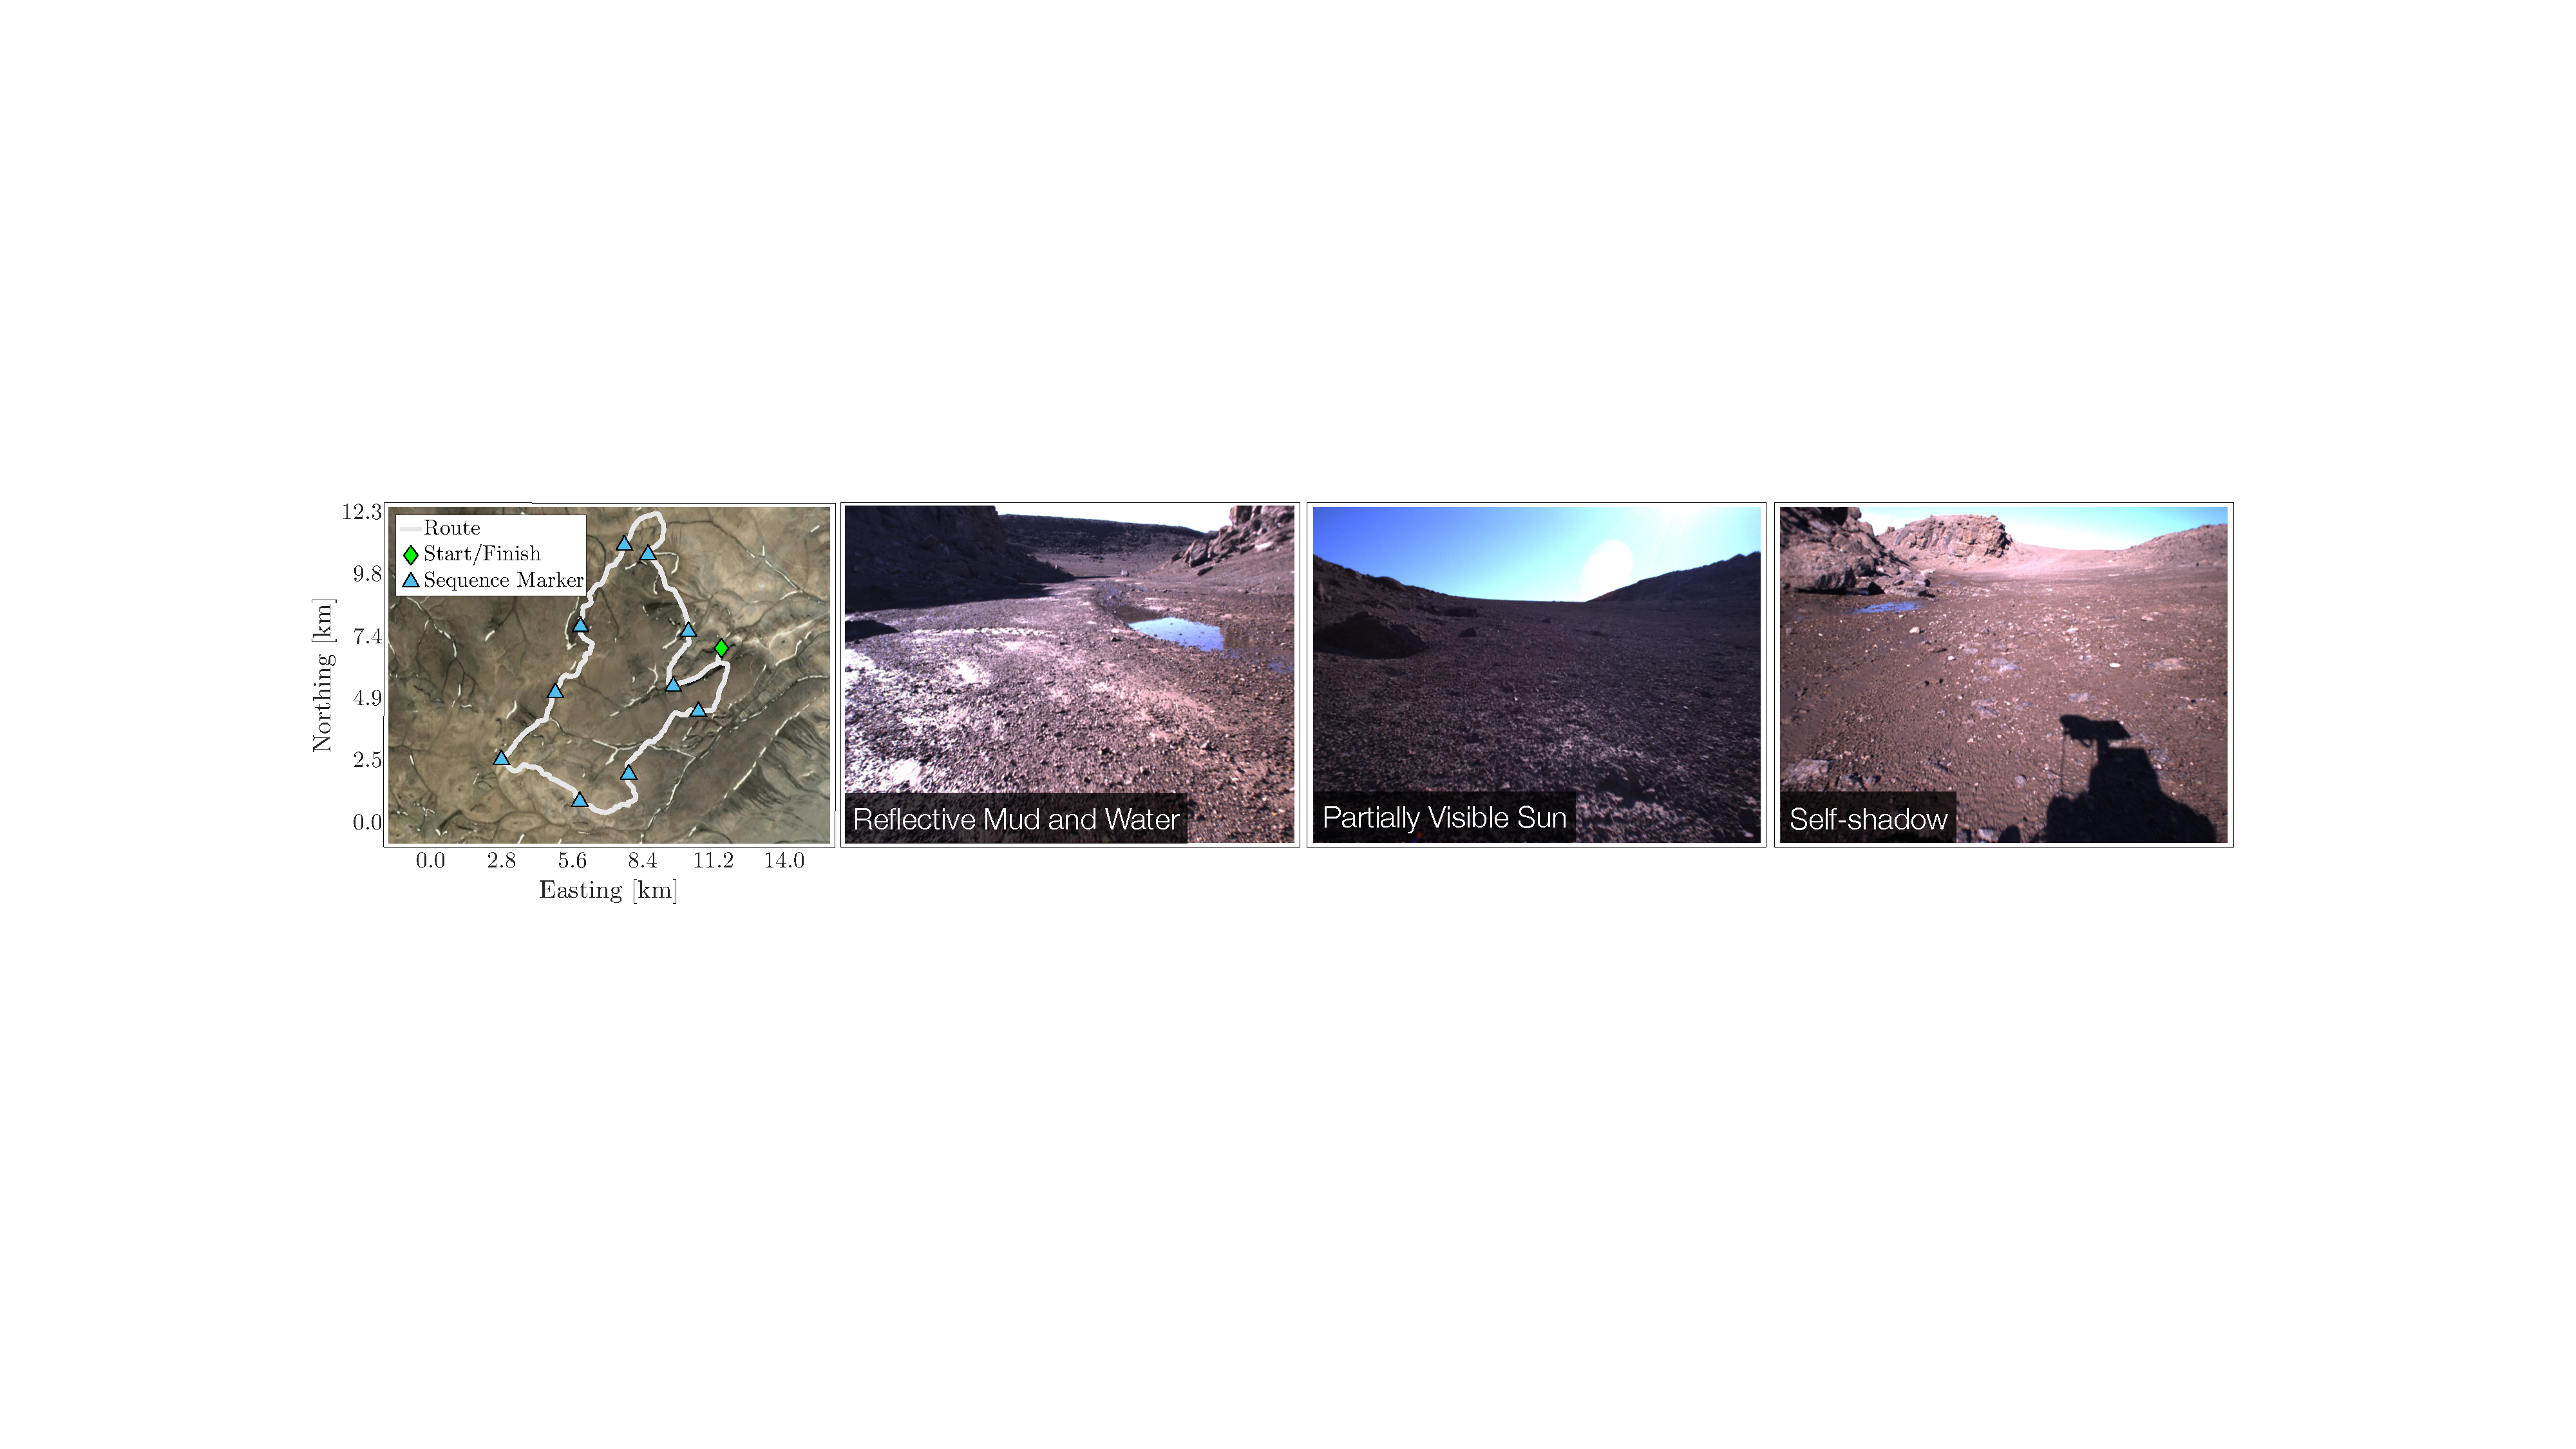
\includegraphics[width=0.99\textwidth]{sun-bcnn/devon/devon_collage.pdf}	
	\caption{GPS track and sample images from the Devon Island traverse, with the start of each sequence highlighted. The Devon Island dataset is conducive to visual sun sensing due to the presence of strong environmental shadows, reflective surfaces such as mud and water, occasionally visible sun, and self-shadowing by the sensor platform. (Map data: Google, DigitalGlobe)}
	\label{fig:devon_collage}
\end{figure*}

\Cref{tab:kitti_test_cnn} summarizes the Sun-BCNN test errors numerically.
Sun-BCNN achieved median vector angle errors of less than 15 degrees on every sequence except sequence \texttt{01} and \texttt{06}, which were particularly difficult in places due to challenging lighting conditions.
It is interesting to note that sequences \texttt{00} and \texttt{06} also have higher than average ANEES values, which indicates that the estimator is overconfident in its estimates despite their low quality.
We suspect this behaviour stems from the assumption of homoscedastic noise in the BCNN, which treats all input images as being equally amenable to sun estimation across the entire sequence.

\subsection{Visual Odometry Experiments}
We evaluated the influence of the estimated sun directions and covariances obtained from Sun-BCNN on the KITTI odometry benchmark using the sun-aided VO pipeline previously described.
To place these results in context, we compare them against the results obtained using simulated sun measurements with varying levels of noise, the method of \citet{Lalonde2011-jw} and its VO-informed variant \citep{2017_Clement_Improving}, and the Sun-CNN of \citet{Ma2016-at}.

\subsubsection{Simulated Sun Sensing} \label{sec:kitti_vo_sim_sun}
In order to gauge the effectiveness of incorporating sun information in each sequence, and to determine the impact of measurement error, we constructed several sets of simulated sun measurements by computing ground truth sun vectors and artificially corrupting them with varying levels of zero-mean Gaussian noise.
We obtained these ground truth sun vectors by transforming the ephemeris vector into each camera frame using ground truth vehicle poses.
Using the same convention as our experiments with simulated trajectories, we created four such measurement sets with $0^\circ$, $10^\circ$, $20^\circ$, and $30^\circ$ mean angular distance from ground truth.

%\vspace{-0.4em}
\Cref{fig:kitti-vo-sim-results} shows the results we obtained using simulated sun measurements on sequence \texttt{05}, in which the basic VO suffers from substantial orientation drift.\footnote{In order to make a fair comparison to the Sun-CNN of \citet{Ma2016-at}, who compute sun directions for every tenth image of the KITTI odometry benchmark, we subsample the sun directions obtained through each other method to match.}
Incorporating absolute orientation information from the simulated sun sensor allows the VO to correct these errors, but the magnitude of the correction decreases as sensor noise increases, consistent with the results of our simulation experiments.
As shown in \Cref{tab:sun-bcnn_kitti_armse}, which summarizes our VO results for all ten sequences, this is typical of sequences where orientation drift is the dominant source of error.

While the VO solutions for sequences such as \texttt{00} do not improve in terms of translational ARMSE, \Cref{tab:sun-bcnn_kitti_armse} shows that rotational ARMSE nevertheless improves on all ten sequences when low-noise simulated sun measurements are included.
This implies that the estimation errors of the basic VO solutions for certain sequences are dominated by non-rotational effects, and that the apparent benefit of the Lalonde method on translational ARMSE in sequence \texttt{00} is likely coincidental.

\subsubsection{Vision-based Sun Sensing} \label{sec:kitti_vo_sim_sun}
\Cref{fig:kitti_arrows} illustrates the behaviour of Sun-BCNN on four characteristic images from test sequence \texttt{05} by overlaying the Sun-BCNN predictions and associated ground truth sun directions for each image.
The two frames in the top row both contain strong shadows which typically result in very accurate sun predictions. 
Conversely, the bottom row highlights two examples of rare situations where ambiguous shadows lead to very inaccurate predictions.
As previously mentioned, we mitigate the influence of these outlier measurements by imposing a robust Huber loss on the sun measurement errors in our optimizer.

\Cref{fig:kitti-vo-results} shows the results we obtained for sequences \texttt{02}, \texttt{05}, and \texttt{08} using the Sun-CNN of \citet{Ma2016-at}, which estimates only the azimuth angle of the sun, our Bayesian Sun-BCNN which provides full 3D estimates of the sun direction as well as a measure of the uncertainty associated with each estimate, and the method of \citet{Lalonde2011-jw} in its original and VO-informed \citep{2017_Clement_Improving} forms, which provide 3D estimates of the sun direction without reasoning about uncertainty.
A selection of results using simulated sun measurements are also displayed for reference.
All four sun detection methods succeed in reducing the growth of total estimation error on this sequence, with Sun-BCNN reducing both translational and rotational error growth significantly more than the other three methods.
Both Sun-CNN and Sun-BCNN outperform the two Lalonde variants, consistent with the results of \citet{Ma2016-at} and \citet{2017_Clement_Improving}.

\Cref{tab:sun-bcnn_kitti_armse} shows results for all ten sequences using each method.
With few exceptions, the VO results using Sun-BCNN achieve improvements in rotational and translational ARMSE comparable to those achieved using the simulated sun measurements with between 10 and 30 degrees average error.
As previously noted, sequences such as \texttt{00} do not benefit significantly from sun sensing since rotational drift is not the dominant source of estimation error in these cases.
Nevertheless, these results indicate that CNN-based sun sensing is a valuable tool for improving localization accuracy in VO and an improvement that comes without the need for additional sensors or a specially oriented camera.

%%%%%%%%%%%%%%%%%%%%%%%%%%%%%%%%%%%%%%%%
% EXPERIMENTS: Devon Island
%%%%%%%%%%%%%%%%%%%%%%%%%%%%%%%%%%%%%%%%
\begin{figure}
    \centering
    \begin{subfigure}[b]{0.75\textwidth}
        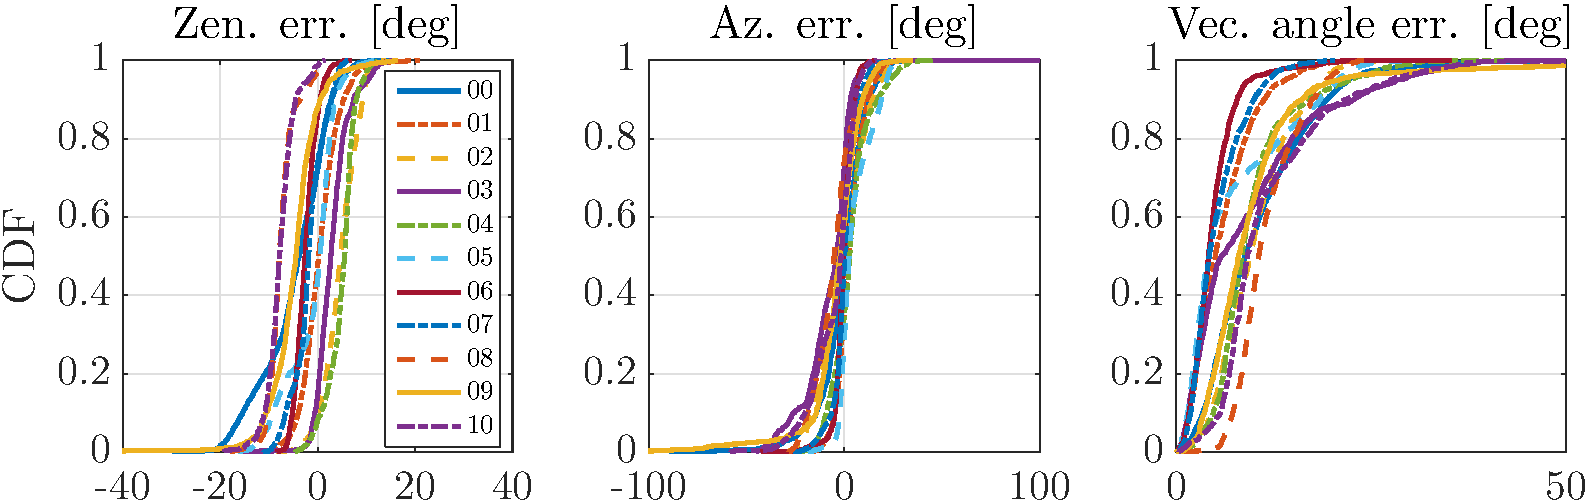
\includegraphics[width=\textwidth]{sun-bcnn/devon/devon_cdf}
    \end{subfigure} 
    \begin{subfigure}[b]{0.75\textwidth}
        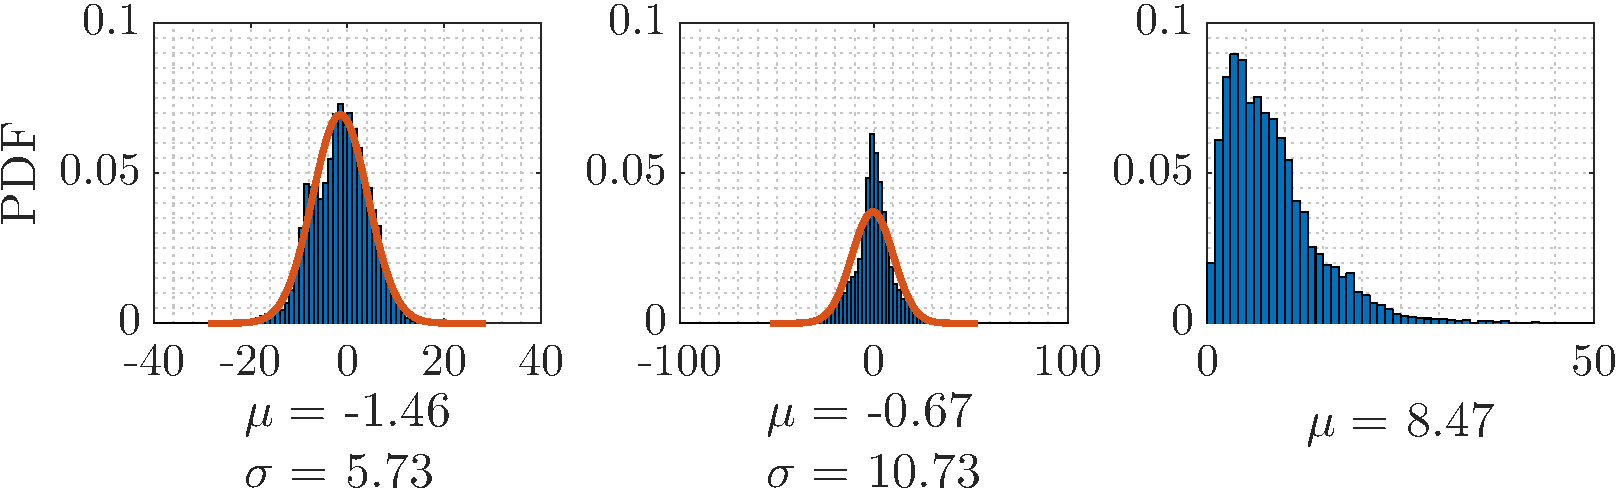
\includegraphics[width=\textwidth]{sun-bcnn/devon/devon_hist_azzen}
    \end{subfigure}
%    \vspace{-0.5em}
    \caption{(Devon Island) Distributions of azimuth error, zenith error, and angular distance for Sun-BCNN compared to ground truth over each test sequence. \emph{Top row}: Cumulative distributions of errors for each test sequence individually. \emph{Bottom row:} Histograms and Gaussian fits of aggregated errors.}
        %\vspace{-0.4em}
    \label{fig:sun-bcnn_devon_cnn_testerrors}
\end{figure}

\begin{figure}
    \centering
    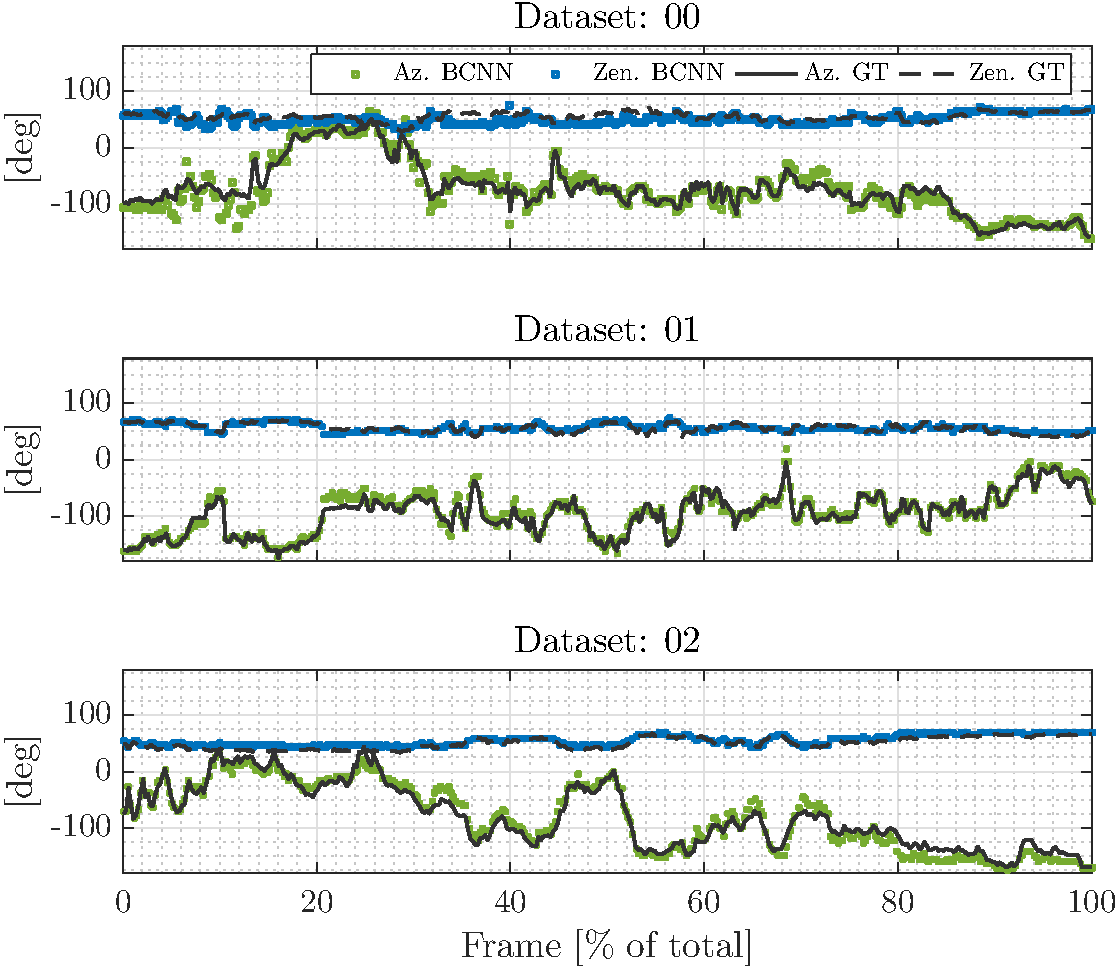
\includegraphics[width=0.75\textwidth]{sun-bcnn/devon/devon_error_over_time_00_01_02}
    \caption{Azimuth (Sun-BCNN azimuth and zenith predictions over time for Devon Island test sequences \texttt{00}, \texttt{01} and \texttt{12}. Sun-BCNN is trained and tested on all frames (in our VO experiments, we use the Sun-BCNN predictions of every tenth image to make a fair comparison). }
    %\vspace{-0.4em}
    \label{fig:sun-bcnn_devon_error_over_time}
\end{figure}

\section{Planetary Analogue Experiments: The Devon Island Rover Navigation Dataset}
In addition to urban driving, we further investigate the usefulness of Sun-BCNN in the context of planetary exploration using the Devon Island Rover Navigation Dataset \citep{Furgale2012-kk}, which consists of various sensor data collected using a mobile sensor platform traversing a 10~km loop on Devon Island in the Canadian High Arctic (\Cref{fig:devon_collage}).
The rugged landscape of Devon Island (\Cref{fig:devon_collage}) is a significant departure from the structured urban environment of Karlsruhe.
Unlike the KITTI odometry benchmark, the Devon Island dataset provides ground truth vehicle orientations for only a small number of images, which means that our previous method of generating ground truth sun vectors using ground truth poses is not applicable.
However, the sensor platform used to collect the dataset was equipped with a hardware sun sensor and inclinometer, both of which were used by \citet{Lambert2012-sn} to correct VO drift.
For our purposes, we ignore the inclinometer and use the sun sensor measurements as training targets for Sun-BCNN.

The Devon Island environment contains many features one might expect to be amenable to visual sun detection.
As shown in \Cref{fig:devon_collage}, the dataset contains strong environmental shadows, stretches of wet terrain featuring reflective mud and water, and some self-shadowing from the sensor platform itself.
At times the sun is partially visible to the camera, although these images tend to be saturated and do not immediately allow for accurate localization of the sun in the image.

For the purposes of our experiments, we partition the dataset into 11 sequences of approximately 1~km each, chosen such that the full pose of the vehicle at the beginning of each sequence is available from the ground truth data (see \Cref{fig:devon_collage}). In aggregate, the sequences contain 13257 poses with associated sun sensor measurements.
We apply a similar training and testing procedure as for the KITTI dataset, with the exception that we now withhold one sequence for validation and hyper-parameter tuning in addition to the sequence withheld for testing.
This leaves nine sequences remaining to form the training sets for each test and validation pair.

\begin{table}[]
\centering
\caption{Test Errors for Sun-BCNN on Devon Island odometry sequences with estimates computed at every image.}
\resizebox{\columnwidth}{!}{%
\label{tab:sun-bcnn_testBCNN_devon}
\begin{threeparttable}
\begin{tabular}{@{}cccccccccccccccc@{}}
         &  & \multicolumn{3}{c}{\textbf{Zenith Error {[}deg{]}}} &  & \multicolumn{3}{c}{\textbf{Azimuth Error {[}deg{]}}} &  & \multicolumn{3}{c}{\textbf{Vector Angle Error {[}deg{]}}} & &  \B \\ \cline{3-5} \cline{7-9} \cline{11-13} 
\textbf{Sequence} &  & Mean          & Median       & Stdev       &  & Mean         & Median        & Stdev        &  & Mean           & Median          & Stdev & & \textbf{ANEES}\tnote{2}         \T \\ \midrule
\texttt{00} &  & -4.77 & -3.77           & 6.82  &  & -0.65 & 0.69           & 12.41 &  & 10.48 & 8.86            & 6.96 &  & 1.27                 \\
\texttt{01} &  & 0.47  & 0.21            & 3.91  &  & 2.96  & 2.31           & 7.01  &  & 5.97  & 5.06            & 4.01 &  & 0.59                 \\
\texttt{02} &  & 4.66  & 4.68            & 3.52  &  & -0.72 & -1.32          & 11.78 &  & 10.02 & 9.51            & 4.76 &  & 1.37                 \\
\texttt{03} &  & 3.09  & 2.70            & 3.41  &  & -7.47 & -4.03          & 12.88 &  & 9.39  & 5.83            & 8.75 &  & 1.11                 \\
\texttt{04} &  & 4.93  & 5.53            & 2.90  &  & 3.27  & 2.72           & 10.09 &  & 9.78  & 8.41            & 5.60 &  & 0.89                 \\
\texttt{05} &  & -1.01 & 0.46            & 4.97  &  & 5.26  & 2.46           & 8.23  &  & 7.19  & 4.15            & 6.60 &  & 0.92                 \\
\texttt{06} &  & -2.45 & -2.58           & 2.23  &  & -0.23 & -0.30          & 5.07  &  & 4.72  & 4.17            & 3.16 &  & 0.31                 \\
\texttt{07} &  & -1.80 & -1.87           & 3.28  &  & 0.47  & 0.20           & 6.45  &  & 5.23  & 4.25            & 3.38 &  & 0.41                 \\
\texttt{08} &  & -7.46 & -7.88           & 2.85  &  & -4.93 & -5.14          & 10.30 &  & 11.61 & 10.63           & 3.96 &  & 1.33                 \\
\texttt{09} &  & -4.72 & -4.46           & 5.27  &  & -3.91 & -2.13          & 14.61 &  & 9.90  & 8.02            & 8.56 &  & 0.86                 \\
\texttt{10} &  & -7.69 & -7.82           & 2.92  &  & -4.81 & -1.54          & 10.80 &  & 11.79 & 9.19            & 7.52 &  & 0.91                 \\ \midrule
  All  &  & -1.46 & -1.23           & 5.73 &  & -0.67 & -0.14         & 10.73 &  & 8.47  & 7.15            & 6.31 &  &  - \\ \bottomrule                   
\end{tabular}
\begin{tablenotes}
	\item[1] We compute Average Normalized Estimation Error Squared (ANEES) values with all sun directions that fall below a cosine distance threshold of $0.3$ (relative to ground truth) and set $\tau^{-1} = 0.01$.
 \end{tablenotes}
\end{threeparttable}
}
\end{table}

\begin{figure}
    \centering
    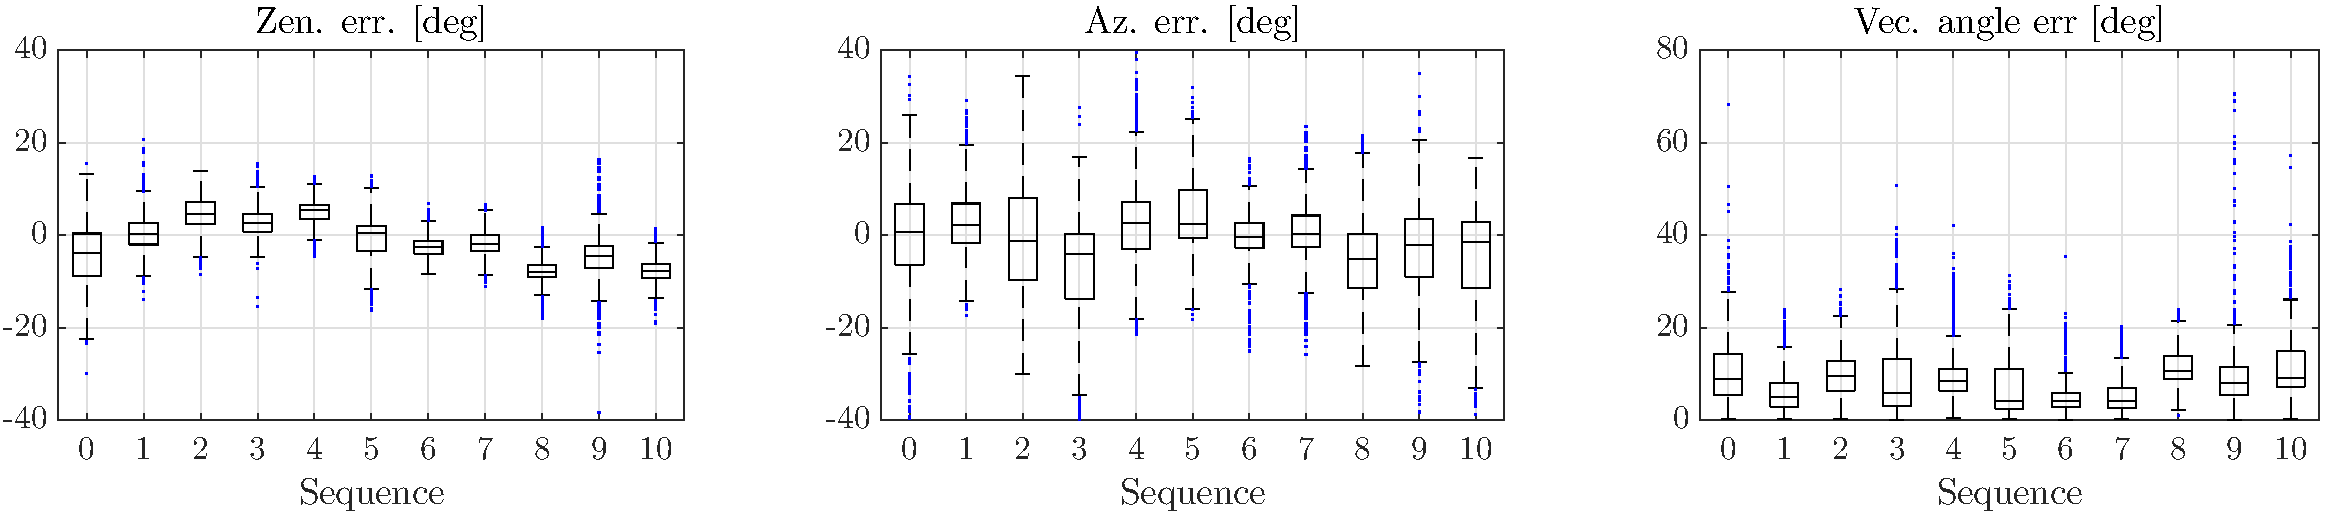
\includegraphics[width=\textwidth]{sun-bcnn/devon/devon_testStatsBoxPlot}
    \caption{Box-and-whiskers plot of final test errors on Devon Island odometry sequences (c.f. \Cref{tab:testBCNN_devon}).}
%    \vspace{-0.4em}
    \label{fig:sun-bcnn_devon_test_error_whiskers}
\end{figure}

\subsection{Sun-BCNN Test Results}
As in our experiments with the KITTI odometry benchmark, we obtained the mean estimated sun vector by evaluating \Cref{eq:sun_direction_mean} with $N=25$ and re-normalizing the resulting vector to preserve unit length. 
To obtain the required covariance on azimuth and zenith angles, we again sampled the vector outputs, converted them to azimuth and zenith angles using \Cref{eq:vec-to-az-zen}, and then applied \Cref{eq:bcnn_covar}.
As shown in \Cref{tab:sun-bcnn_testBCNN_devon}, we chose a value for the model precision $\tau$ such that the Average Normalized Estimation Error Squared (ANEES) of each test sequence is close to one (i.e., the estimator is consistent).

\Cref{fig:sun-bcnn_devon_test_error_whiskers,fig:sun-bcnn_devon_cnn_testerrors} plot the error distributions for azimuth, zenith, and angular distance for all 11 Devon Island odometry sequences, while \Cref{fig:sun-bcnn_devon_error_over_time} shows three characteristic plots of the azimuth and zenith predictions over time. 
We see that the errors in azimuth and zenith are strongly peaked around zero and are better described by a Gaussian distribution than in the case of KITTI (c.f. \Cref{fig:sun-bcnn_kitti_cnn_testerrors}), which as we previously mentioned are important properties assumed by our VO pipeline to appropriately fuse data.
The distribution of zenith errors in the Devon Island dataset does not exhibit the same bias and long tail we observed in the KITTI dataset. 
This is likely because the sun is much lower in the sky (i.e., the zenith angle is further from zero) in the Devon Island dataset than in the KITTI dataset, so there is no clipping of the distribution near zero zenith.

\Cref{tab:sun-bcnn_testBCNN_devon} summarizes the test errors and ANEES of each sequence numerically, while \Cref{fig:sun-bcnn_devon_test_error_whiskers,fig:sun-bcnn_devon_cnn_testerrors} plot the error distributions for azimuth, zenith, and angular distance for each sequence. 
\Cref{fig:sun-bcnn_devon_error_over_time} shows three characteristic plots of the azimuth and zenith predictions over time. 
Sun-BCNN achieved median vector angle errors of less than 10 degrees on every sequence except sequence \texttt{08}.
Consistent with the results we observed in the KITTI experiments, the sequences with the highest median vector angle error (sequences \texttt{02} and \texttt{08}) also have the highest ANEES values, again indicating that the homoscedastic noise assumption is perhaps ill suited to this environment.


\subsection{Visual Odometry Experiments}
As in our KITTI benchmark experiments, we compare visual odometry results on each of our 11 test sequences both with sun-based orientation corrections and without.
Notably, we do not report results using simulated sun measurements since we are unable to generate these measurements without ground truth vehicle orientations for every image.
We also do not report results using the Sun-CNN of \citet{Ma2016-at} since we do not have access to their model.
However, we do compare the results obtained using Sun-BCNN to those obtained using the hardware sun sensor as well as the Lalonde \citep{Lalonde2011-jw} and Lalonde-VO \citep{2017_Clement_Improving} methods.

\begin{figure}
	\centering
	\begin{subfigure}{0.3\textwidth}
%		\vspace{3pt}
    	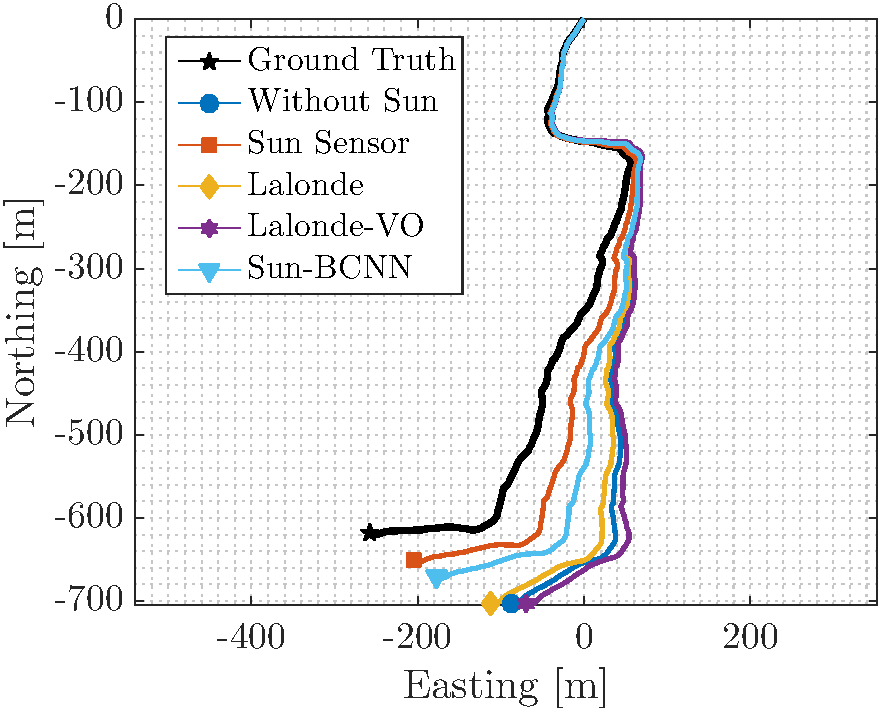
\includegraphics[width=\textwidth]{sun-bcnn/devon/devon_c00_traj}
        \caption{\texttt{00}: VO trajectories (EN-plane)}
        \label{fig:devon_c00_traj}
    \end{subfigure}
    ~
   	\begin{subfigure}{0.3\textwidth}
%		\vspace{6pt}
    	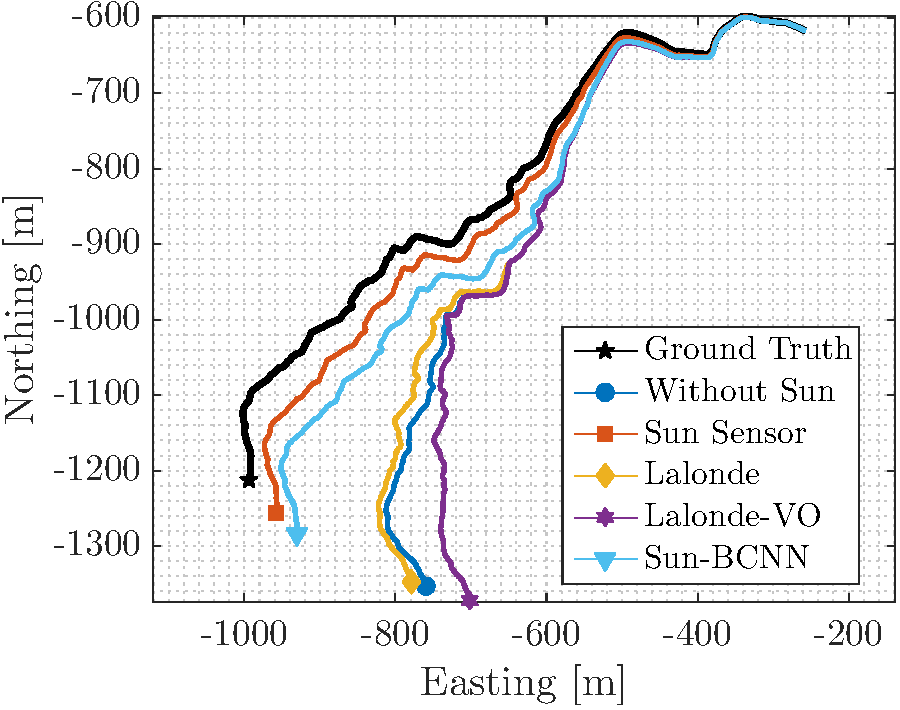
\includegraphics[width=\textwidth]{sun-bcnn/devon/devon_c01_traj}
        \caption{\texttt{01}: VO trajectories (EN-plane)}
        \label{fig:devon_c01_traj}
    \end{subfigure}
    ~
    \begin{subfigure}{0.3\textwidth}
%		\vspace{6pt}
    	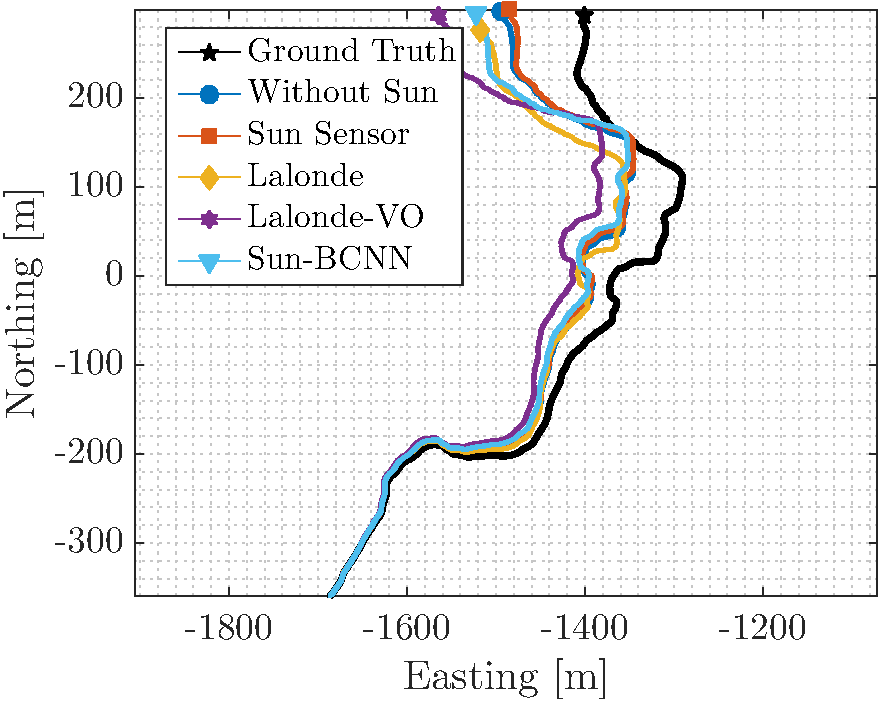
\includegraphics[width=\textwidth]{sun-bcnn/devon/devon_c05_traj}
        \caption{\texttt{05}: VO trajectories (EN-plane)}
        \label{fig:devon_c05_traj}
    \end{subfigure}
    
    \begin{subfigure}{0.3\textwidth}
    	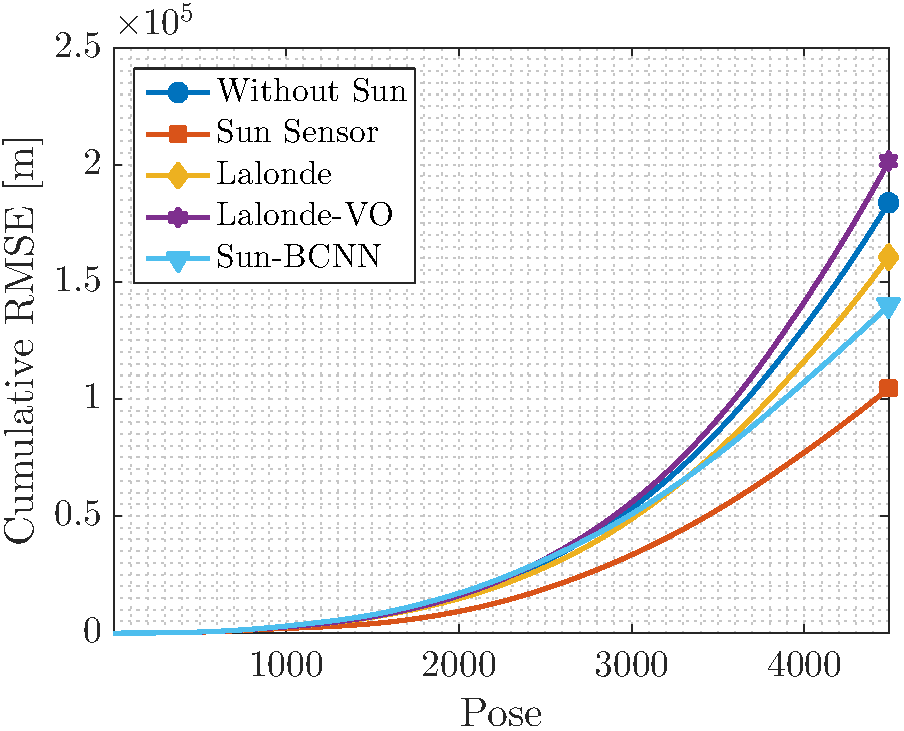
\includegraphics[width=\textwidth]{sun-bcnn/devon/devon_c00_enu_rmse}
        \caption{\texttt{00}: Translational CRMSE}
        \label{fig:devon_c00_transerr_enu}
    \end{subfigure}
    ~
    \begin{subfigure}{0.3\textwidth}
    	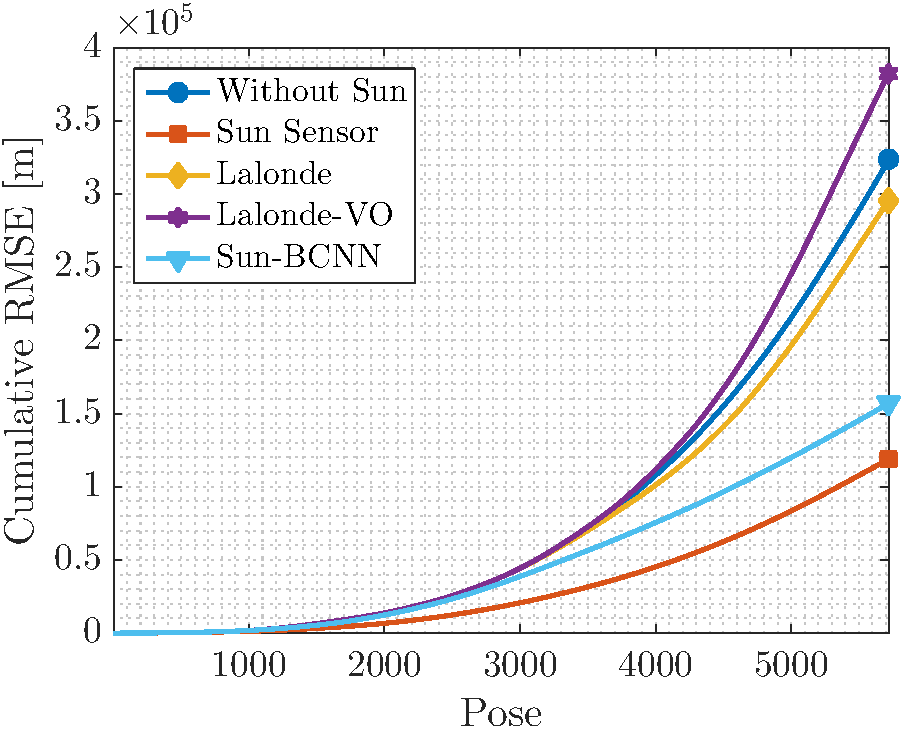
\includegraphics[width=\textwidth]{sun-bcnn/devon/devon_c01_enu_rmse}
        \caption{\texttt{01}: Translational CRMSE}
        \label{fig:devon_c01_transerr_enu}
    \end{subfigure}
    ~
    \begin{subfigure}{0.3\textwidth}
    	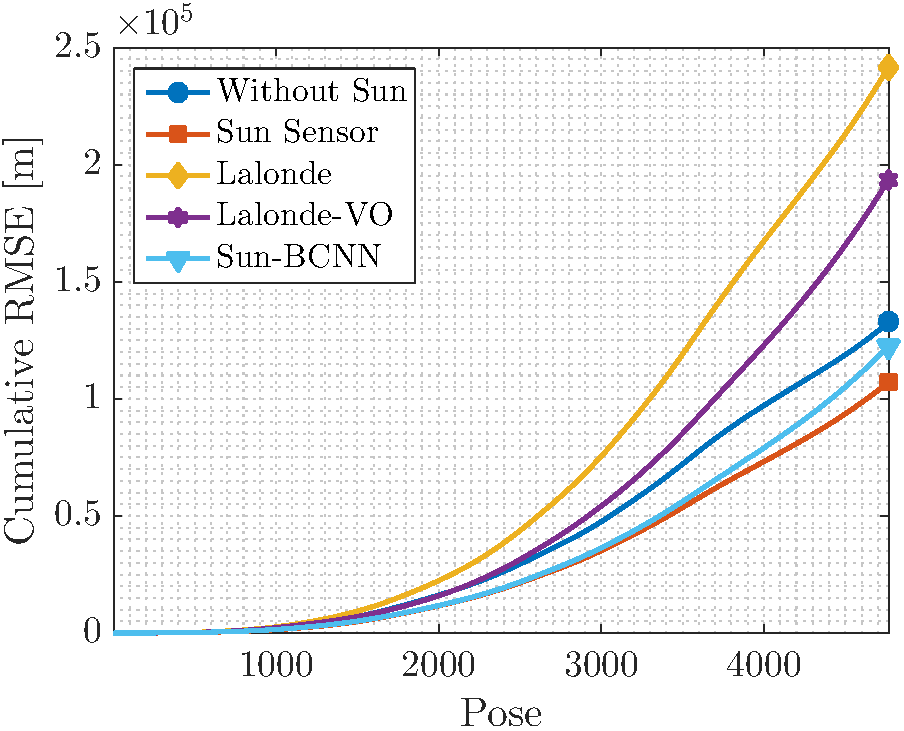
\includegraphics[width=\textwidth]{sun-bcnn/devon/devon_c05_enu_rmse}
        \caption{\texttt{01}: Translational CRMSE}
        \label{fig:devon_c05_transerr_enu}
    \end{subfigure}
    
    \begin{subfigure}{0.3\textwidth}
    	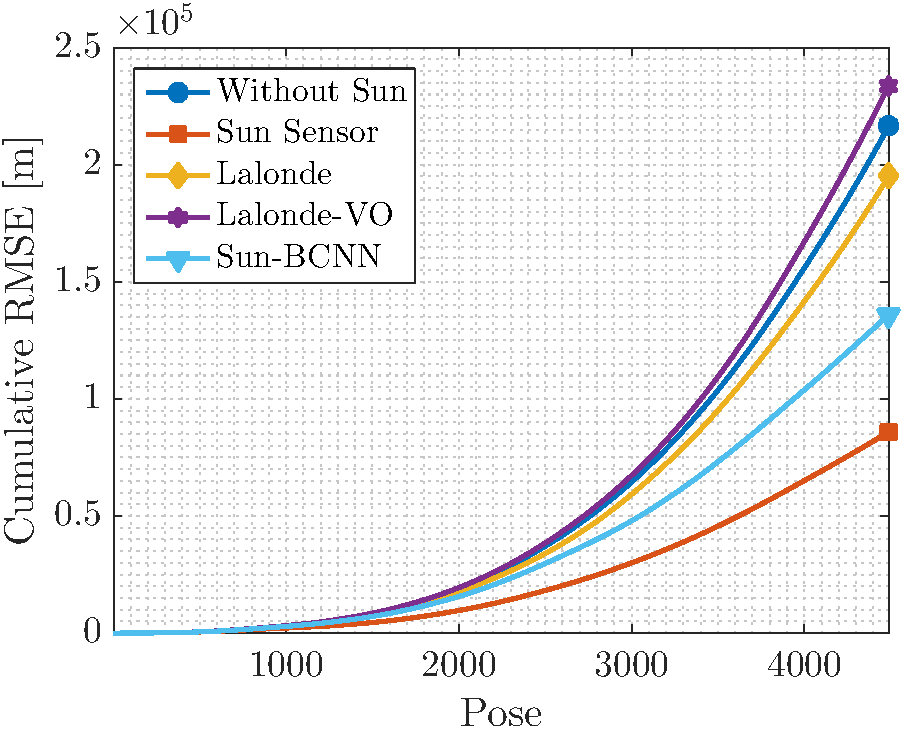
\includegraphics[width=\textwidth]{sun-bcnn/devon/devon_c00_en_rmse}
        \caption{\texttt{00}: Translational CRMSE (EN-Plane)}
        \label{fig:devon_c00_transerr_en}
    \end{subfigure}
    ~
    \begin{subfigure}{0.3\textwidth}
    	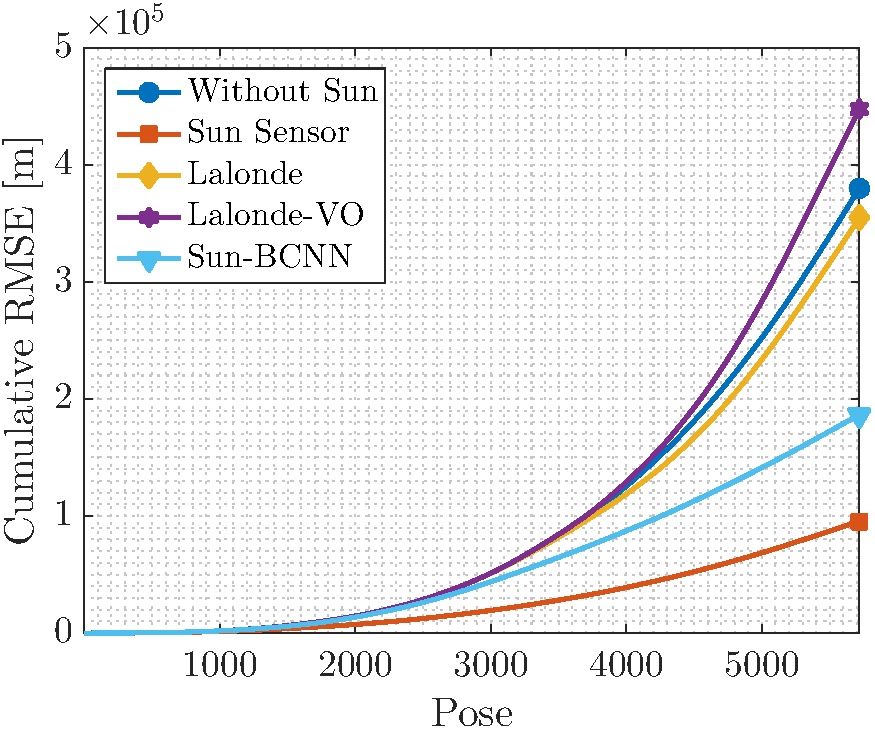
\includegraphics[width=\textwidth]{sun-bcnn/devon/devon_c01_en_rmse}
        \caption{\texttt{01}: Translational CRMSE (EN-Plane)}
        \label{fig:devon_c01_transerr_en}
    \end{subfigure}
    ~
    \begin{subfigure}{0.3\textwidth}
    	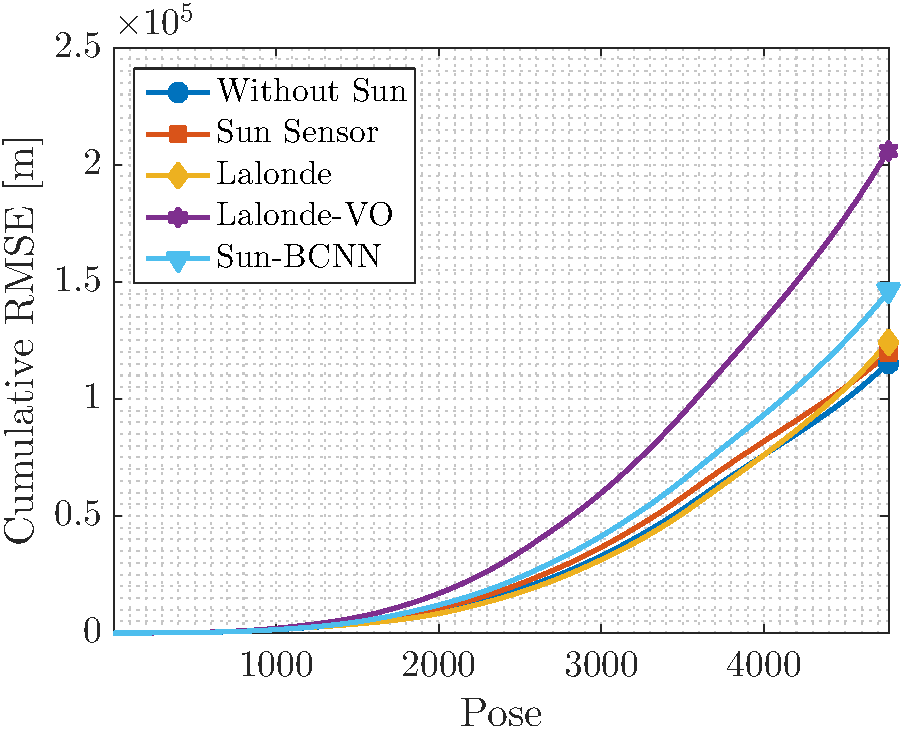
\includegraphics[width=\textwidth]{sun-bcnn/devon/devon_c05_en_rmse}
        \caption{\texttt{05}: Translational CRMSE (EN-Plane)}
        \label{fig:devon_c05_transerr_en}
    \end{subfigure}
    \caption{VO results for Devon Island sequences \texttt{00}, \texttt{01}, and \texttt{05} using estimated sun directions. \emph{Top row}: Estimated and ground truth trajectories in the EN-plane. \emph{Bottom rows}: Translational cumulative root mean squared error (CRMSE). Sun-BCNN significantly reduces the estimation error on sequences where the sun sensing has an impact (c.f. \Cref{tab:devon_armse}).}
    \label{fig:sun-bcnn_devon_vo}
\end{figure}

\begin{table}[h]
\centering
\caption{Comparison of average root mean squared error (ARMSE) on Devon Island sequences with and without sun direction estimates using both a hardware sun sensor and vision-based methods. The best result using a vision-based method is bolded.}
\resizebox{\columnwidth}{!}{%
\label{tab:sun-bcnn_devon_armse}
\begin{tabular}{@{}lccccccccccc@{}}
\textbf{Sequence}                    & \texttt{00} & \texttt{01} & \texttt{02} & \texttt{03} & \texttt{04} & \texttt{05} & \texttt{06} & \texttt{07} & \texttt{08} & \texttt{09}\tnote{1} & \texttt{10} \\ \midrule
\textbf{Length [km]}                 & 0.9         & 1.1         & 1.0         & 1.0         & 0.9         & 1.0         & 1.1         & 1.0         & 0.9         & 0.7         & 0.6         \\ \midrule
\multicolumn{12}{@{}l@{}}{\textbf{Trans. ARMSE [m]}} \\
\quad Without Sun         & 40.93          & 56.51          & 41.58          & 42.04          & 30.52          & 27.82          & 58.91          & 40.04          & 47.22          & 11.39         & 12.94         \T \\
\quad Hardware Sun Sensor & 23.26          & 20.79          & 9.79           & 22.03          & 30.79          & 22.47          & 24.14          & 29.59          & 47.97          & 6.26          & 8.50           \B \\
\quad Lalonde             & 35.77          & 51.74          & 53.32          & 47.00          & 39.55          & 50.70          & 94.77          & 59.37          & \textbf{45.78} & 10.03         & 16.23          \T \\
\quad Lalonde-VO          & 44.83          & 66.91          & 44.17          & 59.84          & 42.87          & 40.62          & 52.16          & 36.04          & 50.52          & 11.34         & 16.74          \\
\quad Sun-BCNN            & \textbf{31.17} & \textbf{27.45} & \textbf{16.00} & \textbf{26.02} & \textbf{29.34} & \textbf{25.70} & \textbf{33.43} & \textbf{32.25} & 50.80          & \textbf{4.27} & \textbf{14.92} \\ \midrule
\multicolumn{12}{@{}l@{}}{\textbf{Trans. ARMSE (EN-plane) [m]}} \\
\quad Without Sun         & 48.20          & 66.49          & 43.58         & 45.92          & 31.08          & 24.23          & 43.01          & 22.33          & 40.85          & 9.30 & 15.59          \T \\
\quad Hardware Sun Sensor & 19.13          & 16.74          & 8.99          & 21.18          & 28.27          & 25.08          & 29.27          & 21.76          & 28.89          & 5.14 & 9.70           \B \\
\quad Lalonde             & 43.45          & 62.03          & 36.21         & 49.44          & \textbf{20.13} & \textbf{26.13} & 53.22          & \textbf{18.10} & 35.62          & 6.01 & 18.45          \T \\
\quad Lalonde-VO          & 52.05          & 78.26          & 40.20         & 59.09          & 50.12          & 43.28          & 53.62          & 42.71          & 49.99          & 11.74& 20.17          \\
\quad Sun-BCNN            & \textbf{30.28} & \textbf{32.65} & \textbf{9.62} & \textbf{14.32} & 33.26          & 30.62          & \textbf{36.44} & 23.18          & \textbf{13.53} & \textbf{4.45} & \textbf{14.75} \\ \bottomrule
\end{tabular}
}
\end{table}

\Cref{fig:sun-bcnn_devon_vo} shows sample VO results on three sequences from the Devon Island dataset using no sun measurements, the hardware sun sensor, Sun-BCNN, and the Lalonde variants.
While the Lalonde methods struggle in this environment, Sun-BCNN yields significant improvements in VO accuracy, nearly on par with those obtained using the hardware sun sensor.

\Cref{tab:sun-bcnn_devon_armse} summarizes these results numerically for all 11 sequences in the dataset.
While the addition of sun sensing using either the hardware sensor or Sun-BCNN generally results in significant reductions in error, we note that in certain cases (e.g., sequence \texttt{05}), sun sensing has little or no impact on the VO result.
We suspect that the translation errors in these cases are dominated by non-rotational effects, similarly to those observed in our experiments with the KITTI dataset, although it is difficult to be certain in the absence of rotational ground truth.
As previously mentioned, the incorporation of a motion prior in the VO estimator would likely reduce the impact of these errors.

%%%%%%%%%%%%%%%%%%%%%%%%%%%%%%%%%%%%%%%%
% SENSITIVITY ANALYSIS
%%%%%%%%%%%%%%%%%%%%%%%%%%%%%%%%%%%%%%%%
\section{Sensitivity Analysis}
In this section we analyze the sensitivity of our model to cloud cover, investigate the possibility of model transfer between urban and planetary analogue environments, and examine the impact of different methods for computing the mean and covariance of a norm-constrained vector on the accuracy and consistency of the estimated sun directions.

%%%%%%%%%%%%%%%%%%%%%%%%%%%%%%%%%%%%%%%%
% SUN/CLOUD
%%%%%%%%%%%%%%%%%%%%%%%%%%%%%%%%%%%%%%%%
\subsection{Cloud Cover}
Given that both the KITTI and Devon Island datasets were collected in sunny conditions, it is natural to wonder whether and to what extent Sun-BCNN is affected by cloud cover. 
As shown in \Cref{fig:sun-bcnn_kitti_cnn_activations}, Sun-BCNN relies in part on shadows and other local illumination variations to estimate the direction of the sun.
Since the diffuse nature of daylight in cloudy conditions tends to soften shadows and other shading variations, one might expect Sun-BCNN to perform worse in cloudy conditions.
Accordingly, we investigated the effect of cloud cover on Sun-BCNN using selected sequences from the Oxford Robotcar Dataset \citep{Maddern2016-ng}, which consists of 1000~km of urban driving along a consistent route but in varying weather conditions and at varying times over the course of a year.

\begin{figure}
    \centering
    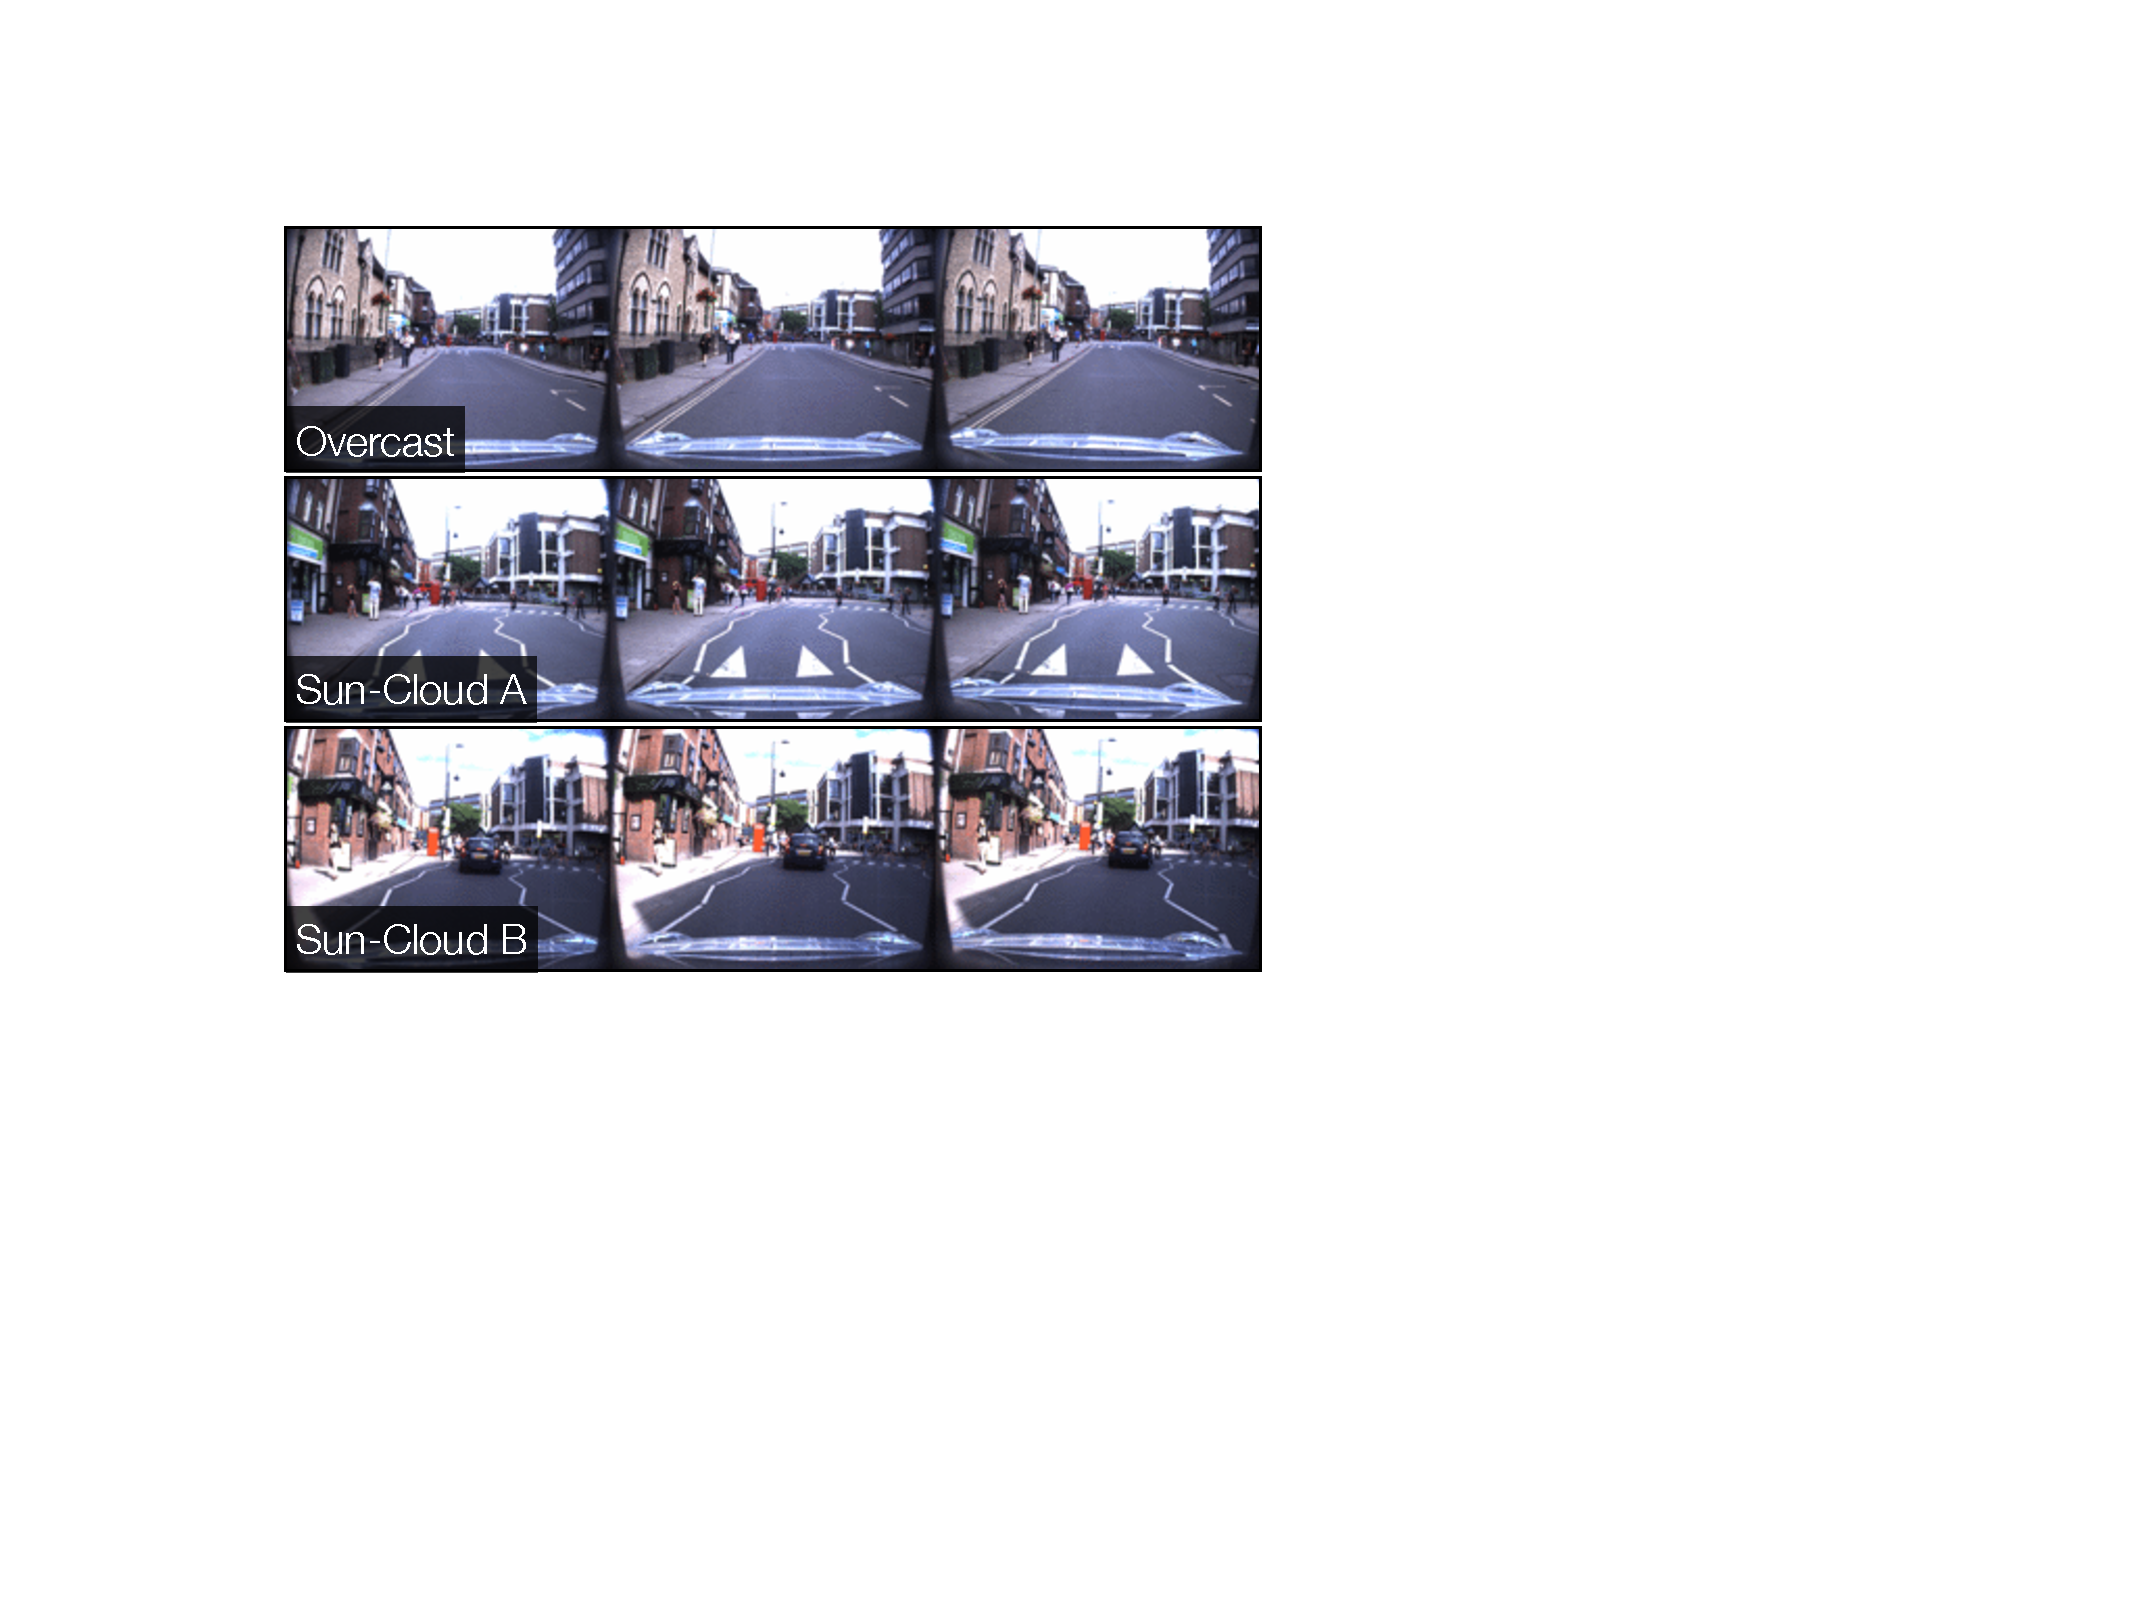
\includegraphics[width=0.7\textwidth]{sun-bcnn/oxford/oxford_oxford-sun-cloud}
    \caption{Sample images of approximately the same location taken from three different Oxford Robotcar sequences we used to investigate the effect of cloud cover on Sun-BCNN.}
    \label{fig:oxford-images}
\end{figure}

\subsubsection{Procedure}
We selected three sequences collected within a two hour period on the same day (namely \texttt{2014-07-14-14-49-50}, \texttt{2014-07-14-15-16-36}, and \texttt{2014-07-14-15-42-55}), which consist of the same route observed under different lighting conditions. 
 \Cref{fig:oxford-images} presents sample images from each of these sequences, which we label \emph{Overcast}, \emph{Sun-Cloud A}, and \emph{Sun-Cloud B}, respectively.
To evaluate the performance of Sun-BCNN in each of these conditions, we partition each sequence into a randomly selected set of training (80\%), validation (10\%) and test (10\%) images, and then train and test Sun-BCNN on each of the nine train-test permutations. 

\subsubsection{Results}

\begin{figure}
    \centering
    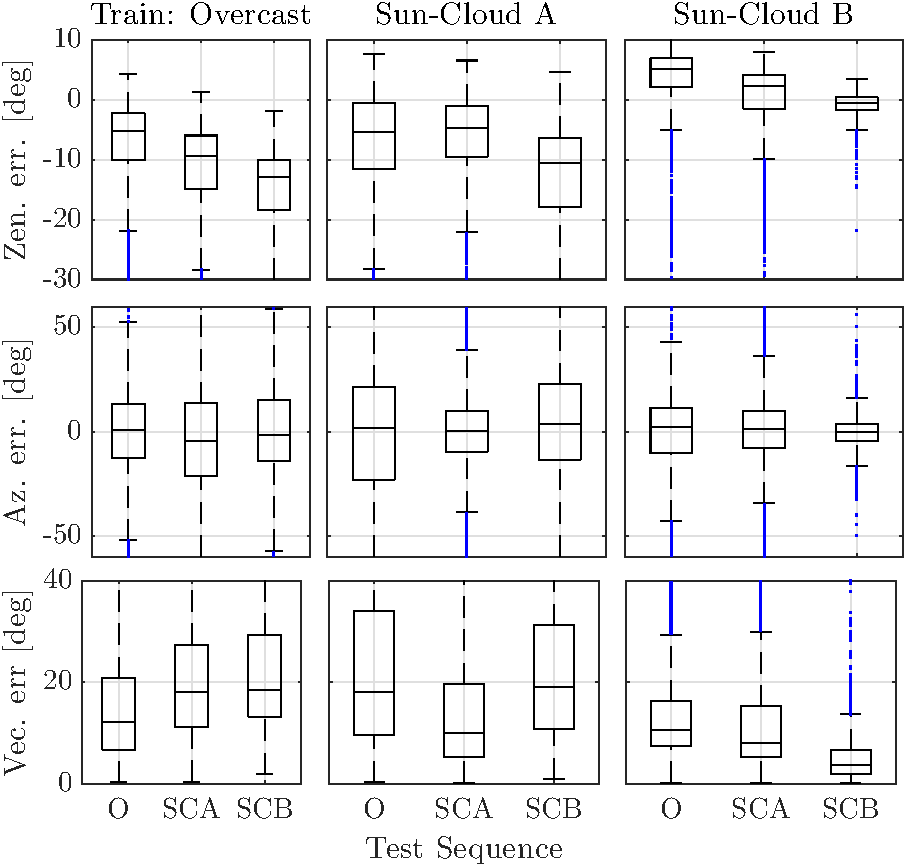
\includegraphics[width=0.75\textwidth]{sun-bcnn/oxford/oxford_boxwhiskers_cloudsunny_comp}
    \caption{Box-and-whiskers plot for zenith, azimuth and vector angle errors for nine different combinations of train-test sequences taken from the Oxford Robotcar dataset.  Each column corresponds to a different training sequence, and each plot contains three different test sequences. In the bottom legend, we use the labels O: \emph{Overcast}, SCA: \emph{Sun-Cloud A}, SCB: \emph{Sun-Cloud B}.}
    \label{fig:oxford-boxwhiskers}
\end{figure}

\Cref{fig:oxford-boxwhiskers} shows the results of these experiments with box and whisker plots for azimuth, zenith and vector angle errors while \Cref{tab:sun-bcnn_testBCNN_oxford_weather} summarizes the results numerically. 
We obtained the most accurate test predictions using the model trained on \emph{Sun-Cloud B}, the sequence with the least amount of cloud cover. 
Notably, this model produced vector angle errors on the  \emph{Overcast} test set that were lower than those trained with its own \emph{Overcast} training set. 
Moreover, we note that the \emph{Sun-Cloud A} model achieved similar test errors when applied to the \emph{Sun-Cloud B} test set as when applied to the \emph{Overcast} test set.
Similarly, the \emph{Sun-Cloud B} model achieved similar test errors when applied to the \emph{Sun-Cloud A} test set as when applied to the \emph{Overcast} test set.
From this we can conclude the following: 1) that Sun-BCNN can still perform well in the presence of cloud cover; and 2) that training in environments illuminated by strong directional light (i.e., sunny conditions) can significantly improve sun estimation accuracy in different test conditions.


%%%%%%%%%%%%%%%%%%%%%%%%%%%%%%%%%%%%%%%%
% TRANSFER LEARNING
%%%%%%%%%%%%%%%%%%%%%%%%%%%%%%%%%%%%%%%%
\subsection{Model Generalization}
It may also be natural to ask how well a Sun-BCNN model trained in an urban environment performs in a planetary analogue environment and vice versa.
This would provide some indication of whether the model generalizes to new environments or if a philosophy of place-specific excellence (e.g., the place-specific visual features of \cite{mcmanus2014}) is more appropriate for the task of illumination estimation.

\subsubsection{Procedure}
We attempted to answer this question by creating three larger datasets from combinations of the sequences used in our previous experiments:
\begin{enumerate}
	\item KITTI odometry sequences \texttt{00} - \texttt{10}; 
	\item Devon Island sequences \texttt{00} - \texttt{10}; and
	\item the previously discussed \emph{Overcast}, \emph{Sun-Cloud A}, and \emph{Sun-Cloud B} sequences from the Oxford Robotcar dataset.
\end{enumerate}
We randomly partitioned each dataset into training (90\%) and test (10\%) sets.
We then trained three separate Sun-BCNN models on each training set, and evaluated each trained model on each of the three test sets.
 
\subsubsection{Results}
\Cref{fig:sun-bcnn_experiment-transfer-boxwhiskers} shows the results of these experiments with box and whisker plots for azimuth, zenith and vector angle errors while \Cref{tab:sun-bcnn_testBCNN_oxford_weather} summarizes the results numerically. 
We see that none of the three models generalize well to environments other than the one in which they were trained, yielding large and significantly biased test errors.
We note, however, that the Oxford model was the least egregious offender, and speculate that this may be because the Oxford sequences contain significantly more training images than the other two datasets (approximately 3 times as many as the KITTI odometry benchmark and 5 times as many as the Devon Island dataset).

A possible explanation for the poor generalization of these models is the fact that each dataset was collected using different cameras with different optical properties and parameter settings.
We believe these differences affect Sun-BCNN's ability to recover an accurate estimate of a three dimensional direction vector, since metrically important quantities such as the principal point and focal length of the sensor can vary significantly from camera to camera. 
Furthermore, differences in dynamic range may also significantly affect the ability of Sun-BCNN to treat shading variations consistently.

\begin{figure}
    \centering
    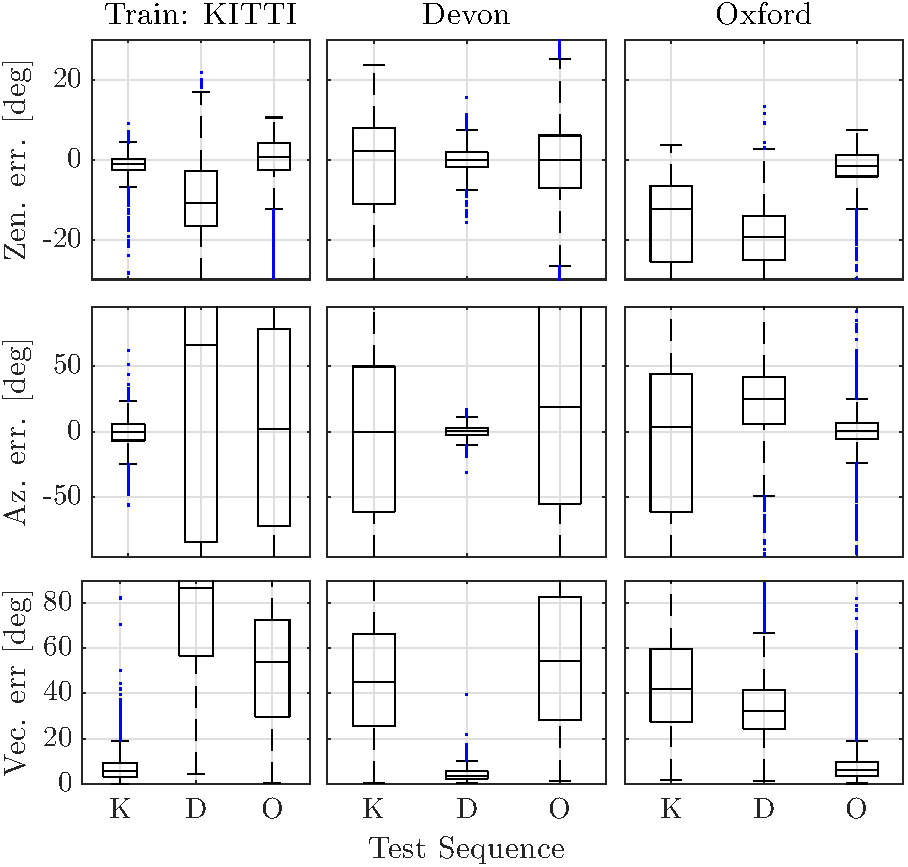
\includegraphics[width=0.75\textwidth]{sun-bcnn/boxwhiskers_transfer_comp}
    \caption{Box-and-whiskers plot for zenith, azimuth and vector angle errors for nine different combinations of train-test datasets.  Each column corresponds to a different training sequence, and each plot contains three different test sequences. In the bottom legend, we use the labels K: KITTI, D: Devon Island, O: Oxford. All three models produce large biased errors when applied to other datasets, likely due to variations in optical properties and parameter settings across cameras.}
%    \vspace{-0.4em}
    \label{fig:sun-bcnn_experiment-transfer-boxwhiskers}
\end{figure}

\begin{table}[]
\centering
\caption{Test Errors for Sun-BCNN on three different Oxford Robotcar sequences collected on the same day with different lighting conditions.}
\label{tab:sun-bcnn_testBCNN_oxford_weather}

\resizebox{\columnwidth}{!}{%
\begin{threeparttable}
\begin{tabular}{@{}llccccccccccc@{}}
&  & \multicolumn{3}{c}{\textbf{Zenith Error {[}deg{]}}} &  & \multicolumn{3}{c}{\textbf{Azimuth Error {[}deg{]}}} &  & \multicolumn{3}{c}{\textbf{Vector Error {[}deg{]}}} \B \\ \cline{3-5} \cline{7-9} \cline{11-13}
\textbf{Train}      & \textbf{Test}  & Mean         & Median       & Std.      &  & Mean        & Median      & Std.       &  & Mean        & Median       & Std.       \T\B \\ \midrule
\multirow{3}{*}{Overcast\tnote{1}}    & Overcast  & -7.12        & -5.20        & 7.04      &  & -0.66       & 0.72        & 29.36      &  & 15.22       & 12.06        & 11.73      \\
                             & Sun-Cloud A  & -11.58       & -9.34        & 7.94      &  & -5.71       & -4.37       & 37.21      &  & 21.19       & 18.03        & 14.07      \\
                             & Sun-Cloud B  & -15.23       & -12.96       & 8.00      &  & 0.05        & -1.49       & 38.83      &  & 23.36       & 18.49        & 15.05      \\ \midrule
\multirow{3}{*}{Sun-Cloud A\tnote{2}} & Overcast  & -7.17        & -5.39        & 9.05      &  & -0.67       & 1.68        & 51.27      &  & 23.66       & 18.03        & 18.11      \\
                             & Sun-Cloud A  & -6.49        & -4.64        & 7.88      &  & 0.29        & 0.35        & 27.42      &  & 14.31       & 10.02        & 12.75      \\
                             & Sun-Cloud B  & -12.89       & -10.58       & 8.94      &  & 1.87        & 3.51        & 40.41      &  & 23.45       & 19.06        & 16.75      \\ \midrule
\multirow{3}{*}{Sun-Cloud B\tnote{3}} & Overcast  & 3.34         & 5.22         & 6.46      &  & -0.32       & 2.24        & 26.07      &  & 13.95       & 10.63        & 11.32      \\
                             & Sun-Cloud A  & -0.14        & 2.30         & 7.36      &  & -1.08       & 1.34        & 28.54      &  & 13.76       & 8.06         & 14.60      \\
                             & Sun-Cloud B  & -0.84        & -0.54        & 2.07      &  & -0.36       & -0.22       & 9.00       &  & 5.11        & 3.73         & 5.13      \\ \bottomrule
\end{tabular}
\begin{tablenotes}
	\item \tnote{1} \texttt{2014-07-14-14-49-50} \quad \tnote{2} \texttt{2014-07-14-15-16-36} \quad \tnote{3} \texttt{2014-07-14-15-42-55}
\end{tablenotes}
\end{threeparttable}
}
\end{table}

\begin{table}[]
\centering
\caption{Test Errors for Sun-BCNN on different training and test datasets.}
\label{tab:sun-bcnn_testBCNN_transfer_experiment}
\resizebox{\columnwidth}{!}{%
\begin{tabular}{@{}llccccccccccc@{}}
&  &  \multicolumn{3}{c}{\textbf{Zenith Error {[}deg{]}}} &  & \multicolumn{3}{c}{\textbf{Azimuth Error {[}deg{]}}} &  & \multicolumn{3}{c}{\textbf{Vector Error {[}deg{]}}} \B \\ \cline{3-5} \cline{7-9} \cline{11-13}
\textbf{Train}      & \textbf{Test}   & Mean         & Median       & Std.      &  & Mean        & Median      & Std.       &  & Mean        & Median       & Std.       \T\B \\ \midrule
\multirow{3}{*}{KITTI}        & KITTI          & -1.49        & -1.08       & 2.99       &  & -0.64      & -0.60       & 11.46       &  & 7.16        & 5.61         & 6.23       \\
                              & Devon Island   & -9.27        & -10.86      & 9.97       &  & 26.78      & 66.15       & 113.23      &  & 81.32       & 86.82        & 33.48      \\
                              & Oxford         & -0.02        & 0.80        & 6.59       &  & -0.44      & 1.81        & 91.30       &  & 52.39       & 54.05        & 29.46      \\ \midrule
\multirow{3}{*}{Devon Island} & KITTI          & -2.37        & 2.27        & 14.30      &  & -5.58      & -0.38       & 78.01       &  & 48.16       & 45.06        & 27.85      \\
                              & Devon Island   & -0.08        & -0.05       & 3.20       &  & 0.20       & 0.12        & 5.52        &  & 4.24        & 3.52         & 2.96       \\
                              & Oxford         & -1.35        & 0.00        & 11.57      &  & 17.12      & 18.85       & 96.86       &  & 55.52       & 54.55        & 29.88      \\ \midrule
\multirow{3}{*}{Oxford}       & KITTI          & -17.05       & -12.25      & 13.19      &  & -6.94      & 3.55        & 77.70       &  & 44.66       & 41.91        & 23.00      \\
                              & Devon Island   & -20.07       & -19.47      & 9.81       &  & 20.92      & 24.56       & 45.52       &  & 35.16       & 32.15        & 16.07      \\
                              & Oxford         & -1.96        & -1.59       & 4.60       &  & 0.19       & 0.48        & 15.08       &  & 8.08        & 6.16         & 7.68      \\ \bottomrule
\end{tabular}
}
\end{table}

%%%%%%%%%%%%%%%%%%%%%%%%%%%%%%%%%%%%%%%%
% COVARIANCE
%%%%%%%%%%%%%%%%%%%%%%%%%%%%%%%%%%%%%%%%
\subsection{Mean and Covariance Computation}
In our formulation, Sun-BCNN outputs a sampling of unit-norm 3D vectors. 
Due to the unit-norm constraint, it is not immediately clear how to apply \Cref{eq:bcnn_covar,eq:sun_direction_mean} to calculate the mean and covariance of these samples.
In this section we present and empirically evaluate two possible procedures for each computation using the previously discussed combined datasets for KITTI, Devon Island, and Oxford.

\subsubsection{Mean computation}
\paragraph{Procedure}
We investigated two different methods for computing the mean of the sampled sun vectors, which we refer to as \emph{Method I} and \emph{Method II}. 

\begin{enumerate} 
\item In \emph{Method I} (used in this work), we first evaluate \Cref{eq:sun_direction_mean} directly on the constrained unit vectors produced by $N$ stochastic passes through the BCNN. We then re-normalize the resulting mean vector to enforce unit length, and convert it to azimuth and zenith angles using \Cref{eq:vec-to-az-zen}.
\item In \emph{Method II}, we first convert each of the $N$ unit vectors produced through stochastic passes through the BCNN to azimuth and zenith angles using \Cref{eq:vec-to-az-zen}. We then evaluate \Cref{eq:sun_direction_mean} on the angles themselves to obtain the mean in azimuth-zenith coordinates.
\end{enumerate}

We evaluated both methods using the same combined datasets and partitioning scheme as in the transfer learning experiment previously presented.

\paragraph{Results}
\Cref{tab:mean_estimation_comp} presents the azimuth, zenith and vector errors for the two mean computation methods. 
\emph{Method I} produces lower vector errors and smaller standard deviations in azimuth and zenith on all three datasets.

\begin{table}[]
\centering
\caption{A comparison of prediction errors from different mean estimation methods.}
\label{tab:mean_estimation_comp}
\resizebox{\columnwidth}{!}{%
\begin{tabular}{@{}ccccccccccccc@{}}
 &  & \multicolumn{3}{c}{\textbf{Zenith Error {[}deg{]}}} &  & \multicolumn{3}{c}{\textbf{Azimuth Error {[}deg{]}}} &  & \multicolumn{3}{c}{\textbf{Vector Error {[}deg{]}}} \B \\ \cline{3-5} \cline{7-9} \cline{11-13}
                      \textbf{Sequence}    &    \textbf{Mean Type}                               & Mean         & Median        & Std.        &  & Mean         & Median        & Std.         &  & Mean         & Median        & Std.        \T\B \\ \midrule
\multirow{2}{*}{KITTI}    & Method I                            & -1.50        & -1.06         & 2.96        &  & -0.56        & -0.47         & 11.52        &  & 7.16         & 5.52          & 6.27        \\ 
                          & Method II                            & -1.06        & -0.76         & 2.44        &  & -0.30        & -0.37         & 30.18        &  & 11.49        & 5.95          & 18.60       \\ \midrule
\multirow{2}{*}{Devon}    & Method I                            & -0.07        & 0.02          & 3.18        &  & 0.19         & 0.27          & 5.76         &  & 4.22         & 3.55          & 3.04        \\ 
                          & Method II                            & 0.04         & 0.09          & 3.17        &  & 1.11         & 0.26          & 24.62        &  & 9.19         & 4.05          & 20.22       \\ \midrule
\multirow{2}{*}{Oxford}   & Method I                            & -1.97        & -1.66         & 4.59        &  & 0.20         & 0.51          & 15.31        &  & 8.12         & 6.10          & 7.74        \\
                          & Method II                            & -1.45        & -1.27         & 3.95        &  & -1.58        & 0.11          & 34.46        &  & 13.18        & 6.76          & 19.24       \\ \bottomrule
\end{tabular}
}
\end{table}

\begin{table}[]
\centering
\caption{A comparison of ANEES values for different mean and covariance propagation methods.}
\label{tab:sun-bcnn_cov_estimation_comp}
\begin{tabular}{@{}lllcc@{}}
\textbf{Sequence}                & \textbf{Covariance Type}              &   \textbf{Mean Type}   &  & \textbf{ANEES} \\ \midrule
\multirow{4}{*}{KITTI}  & \multirow{2}{*}{Method I} &  Method I &  & 0.95  \\
                        &                         &   Method II &  & 5.10  \B \\  
                        
                        & \multirow{2}{*}{Method II} &  Method I &  & 1.40  \T \\
                        &                         &   Method II &  & 0.87  \\ \midrule
                        
\multirow{4}{*}{Devon}  & \multirow{2}{*}{Method I} &   Method I &  & 1.29   \\
                        &                         &   Method II &  & 10.05 \B \\
                        
                        & \multirow{2}{*}{Method II} &   Method I &  & 0.50  \T\\
                        &                         &   Method II &  & 0.85  \\ \midrule
                        
\multirow{4}{*}{Oxford} & \multirow{2}{*}{Method I} &   Method I &  & 1.50  \\
                        &                         &   Method II &  & 2.14  \B \\
                        & \multirow{2}{*}{Method II} &   Method I &  & 1.30  \T \\
                        &                         &   Method II &  & 0.89  \\ \bottomrule
\end{tabular}
\end{table}

\subsubsection{Covariance Computation}
\paragraph{Procedure}
We further investigated two different covariance computation methods, which we also refer to as \emph{Method I} and \emph{Method II}. 

\begin{enumerate} 
\item In \emph{Method I}, we first evaluate \Cref{eq:bcnn_covar} directly on the constrained unit vectors produced by $N$ stochastic passes through the BCNN, yielding a $3 \times 3$ covariance. 
We then compute a $2 \times 2$ covariance on azimuth and zenith by propagating the $3 \times 3$ covariance through a linearized \Cref{eq:vec-to-az-zen}.

\item In \emph{Method II} (used in this work), we first convert each of the $N$ unit vectors produced by stochastic passes through the BCNN to azimuth and zenith angles, and then evaluate \Cref{eq:bcnn_covar} on the angles themselves.
\end{enumerate}

We once again re-used the transfer learning datasets with the same partitioning scheme, and evaluated covariances on the test sets corresponding to each of the three models. 
To control for the effect of tuning the model precision $\tau$, we replace the diagonal elements of each covariance matrix with the diagonal elements of the empirical covariance corresponding to the entire test set (computed based ground truth azimuth and zenith errors). 
We then compared the consistency of the cross-correlations of each method (i.e., the off-diagonal components of the covariance matrix) by computing ANEES values over the each model's corresponding test set using both mean computation methods.  



\paragraph{Results}
\Cref{tab:sun-bcnn_cov_estimation_comp} lists the ANEES values produced by each method of covariance computation when paired with each mean computation method. 
\emph{Method I} covariances produced better ANEES values when paired with \emph{Method I} mean estimation, but \emph{Method II} covariances paired well with either mean estimation scheme. 



\section{Summary}

In summary, with Sun-BCNN, we applied learned \textit{pseudo-sensors} to the problem of illumination direction in outdoor environments. Sun-BCNN presented
\begin{enumerate}
\item the application of a Bayesian CNN to the problem of sun direction estimation, incorporating the resulting covariance estimates into a visual odometry pipeline; 
\item an empirical demonstration that a Bayesian CNN with dropout layers after each convolutional and fully-connected layer can achieve state-of-the-art accuracy at test time;
\item a loss function that incorporated a 3D unit-length sun direction vector, appropriate for full 6-DOF pose estimation;
\item experimental results on over 30~km of visual navigation data in urban \citep{Geiger2013-ky} and planetary analogue \citep{Furgale2012-kk} environments; 
\item an investigation into the sensitivity of the Bayesian CNN-based sun estimate to cloud cover, camera and environment changes, and measurement parameterization; and
\item open-source software\footnote{\url{https://github.com/utiasSTARS/sun-bcnn-vo}.}.
\end{enumerate}

